\documentclass[letterpaper,12pt,numbered,print,index, oneside]{Classes/PhDThesisPSnPDF}

% `oneside' or `twoside'(default): Printing double side (twoside) or single
% side.
%
% `print': Use `print' for print version with appropriate margins and page
% layout. Leaving the options field blank will activate Online version.
%
% `index': For index at the end of the thesis
%
% `draftclassic': For draft mode without loading any images (same as draft in book)
%
% `draft': Special draft mode with line numbers, images, and water mark with
% timestamp and custom text. Position of the text can also be modified.
%
% `abstract': To generate only the title page and abstract page with
% dissertation title and name, to submit to the Student Registry
%
% `chapter`: This option enables only the specified chapter and it's references
%  Useful for review and corrections.
%
% ************************* Custom Page Margins ********************************
%
% `custommargin`: Use `custommargin' in options to activate custom page margins,
% which can be defined in the preamble.tex. Custom margin will override
% print/online margin setup.
%
% *********************** Choosing the Fonts in Class Options ******************
%
% `times' : Times font with math support. (The Cambridge University guidelines
% recommend using times)
%
% `fourier': Utopia Font with Fourier Math font (Font has to be installed)
%            It's a free font.
%
% `customfont': Use `customfont' option in the document class and load the
% package in the preamble.tex
%
% default or leave empty: `Latin Modern' font will be loaded.
%
% ********************** Choosing the Bibliography style ***********************
%
% `authoryear': For author-year citation eg., Krishna (2013)
%
% `numbered': (Default Option) For numbered and sorted citation e.g., [1,5,2]
%
% `custombib': Define your own bibliography style in the `preamble.tex' file.
%              `\RequirePackage[square, sort, numbers, authoryear]{natbib}'.
%              This can be also used to load biblatex instead of natbib
%              (See Preamble)
%
% **************************** Choosing the Page Style *************************
%
% `default (leave empty)': For Page Numbers in Header (Left Even, Right Odd) and
% Chapter Name in Header (Right Even) and Section Name (Left Odd). Blank Footer.
%
% `PageStyleI': Chapter Name next & Page Number on Even Side (Left Even).
% Section Name & Page Number in Header on Odd Side (Right Odd). Footer is empty.
%
% `PageStyleII': Chapter Name on Even Side (Left Even) in Header. Section Number
% and Section Name in Header on Odd Side (Right Odd). Page numbering in footer

% Uncomment to change page style
%\pagestyle{PageStyleII}

% ********************************** Preamble **********************************
% Preamble: Contains packages and user-defined commands and settings
% ******************************************************************************
% ****************************** Custom Margin *********************************

% Add `custommargin' in the document class options to use this section
% Set {innerside margin / outerside margin / topmargin / bottom margin}  and
% other page dimensions
\ifsetCustomMargin
  \RequirePackage[left=37mm,right=30mm,top=35mm,bottom=30mm]{geometry}
  \setFancyHdr % To apply fancy header after geometry package is loaded
\fi

% Add spaces between paragraphs
%\setlength{\parskip}{0.5em}
% Ragged bottom avoids extra whitespaces between paragraphs
\raggedbottom
% To remove the excess top spacing for enumeration, list and description
%\usepackage{enumitem}
%\setlist[enumerate,itemize,description]{topsep=0em}

% *****************************************************************************
% ******************* Fonts (like different typewriter fonts etc.)*************

% Add `customfont' in the document class option to use this section

\ifsetCustomFont
  % Set your custom font here and use `customfont' in options. Leave empty to
  % load computer modern font (default LaTeX font).
  %\RequirePackage{helvet}

  % For use with XeLaTeX
  %  \setmainfont[
  %    Path              = ./libertine/opentype/,
  %    Extension         = .otf,
  %    UprightFont = LinLibertine_R,
  %    BoldFont = LinLibertine_RZ, % Linux Libertine O Regular Semibold
  %    ItalicFont = LinLibertine_RI,
  %    BoldItalicFont = LinLibertine_RZI, % Linux Libertine O Regular Semibold Italic
  %  ]
  %  {libertine}
  %  % load font from system font
  %  \newfontfamily\libertinesystemfont{Linux Libertine O}
\fi

% *****************************************************************************
% **************************** Custom Packages ********************************

% ************************* Algorithms and Pseudocode **************************

%\usepackage{algpseudocode}


% ********************Captions and Hyperreferencing / URL **********************

% Captions: This makes captions of figures use a boldfaced small font.
%\RequirePackage[small,bf]{caption}

\RequirePackage[labelsep=space,tableposition=top]{caption}
\renewcommand{\figurename}{Fig.} %to support older versions of captions.sty


% *************************** Graphics and figures *****************************

%\usepackage{rotating}
%\usepackage{wrapfig}

% Uncomment the following two lines to force Latex to place the figure.
% Use [H] when including graphics. Note 'H' instead of 'h'
%\usepackage{float}
%\restylefloat{figure}

% Subcaption package is also available in the sty folder you can use that by
% uncommenting the following line
% This is for people stuck with older versions of texlive
%\usepackage{sty/caption/subcaption}
% \usepackage{subcaption}
\usepackage{subfig}
% ********************************** Tables ************************************
\usepackage{booktabs} % For professional looking tables
\usepackage{multirow}

%\usepackage{multicol}
%\usepackage{longtable}
%\usepackage{tabularx}


% *********************************** SI Units *********************************
\usepackage{siunitx} % use this package module for SI units


% ******************************* Line Spacing *********************************

% Choose linespacing as appropriate. Default is one-half line spacing as per the
% University guidelines

% \doublespacing
% \onehalfspacing
% \singlespacing


% ************************ Formatting / Footnote *******************************

% Don't break enumeration (etc.) across pages in an ugly manner (default 10000)
%\clubpenalty=500
%\widowpenalty=500

%\usepackage[perpage]{footmisc} %Range of footnote options


% *****************************************************************************
% *************************** Bibliography  and References ********************

%\usepackage{cleveref} %Referencing without need to explicitly state fig /table

% Add `custombib' in the document class option to use this section
\ifuseCustomBib
   \RequirePackage[square, sort, numbers, authoryear]{natbib} % CustomBib

% If you would like to use biblatex for your reference management, as opposed to the default `natbibpackage` pass the option `custombib` in the document class. Comment out the previous line to make sure you don't load the natbib package. Uncomment the following lines and specify the location of references.bib file

%\RequirePackage[backend=biber, style=numeric-comp, citestyle=numeric, sorting=nty, natbib=true]{biblatex}
%\addbibresource{References/references} %Location of references.bib only for biblatex, Do not omit the .bib extension from the filename.

\fi

% changes the default name `Bibliography` -> `References'
\renewcommand{\bibname}{References}

\renewcommand\chaptername{Capítulo} 
% ******************************************************************************
% ************************* User Defined Commands ******************************
% ******************************************************************************

% *********** To change the name of Table of Contents / LOF and LOT ************

%\renewcommand{\contentsname}{My Table of Contents}
%\renewcommand{\listfigurename}{My List of Figures}
%\renewcommand{\listtablename}{My List of Tables}


% ********************** TOC depth and numbering depth *************************

\setcounter{secnumdepth}{3}
\setcounter{tocdepth}{3}


% ******************************* Nomenclature *********************************

% To change the name of the Nomenclature section, uncomment the following line

%\renewcommand{\nomname}{Symbols}


% ********************************* Appendix ***********************************

% The default value of both \appendixtocname and \appendixpagename is `Appendices'. These names can all be changed via:

%\renewcommand{\appendixtocname}{List of appendices}
%\renewcommand{\appendixname}{Appndx}

% *********************** Configure Draft Mode **********************************

% Uncomment to disable figures in `draft'
%\setkeys{Gin}{draft=true}  % set draft to false to enable figures in `draft'

% These options are active only during the draft mode
% Default text is "Draft"
%\SetDraftText{DRAFT}

% Default Watermark location is top. Location (top/bottom)
%\SetDraftWMPosition{bottom}

% Draft Version - default is v1.0
%\SetDraftVersion{v1.1}

% Draft Text grayscale value (should be between 0-black and 1-white)
% Default value is 0.75
%\SetDraftGrayScale{0.8}


% ******************************** Todo Notes **********************************
%% Uncomment the following lines to have todonotes.

%\ifsetDraft
%	\usepackage[colorinlistoftodos]{todonotes}
%	\newcommand{\mynote}[1]{\todo[author=kks32,size=\small,inline,color=green!40]{#1}}
%\else
%	\newcommand{\mynote}[1]{}
%	\newcommand{\listoftodos}{}
%\fi

% Example todo: \mynote{Hey! I have a note}

% *****************************************************************************
% ******************* Better enumeration my MB*************
\usepackage{enumitem}

% \usepackage{algpseudocode}
% \usepackage[linesnumbered,lined,commentsnumbered]{algorithm2e}
% \usepackage{algorithmic}
%Mis paquetes
\usepackage[spanish]{babel}
\usepackage[final]{pdfpages}
\usepackage{algorithm}
\usepackage{algorithmic}
\usepackage{mwe}
\usepackage[table,xcdraw]{xcolor}


\newlength{\tempdima}
\newcommand{\rowname}[1]% #1 = text
{\rotatebox{90}{\makebox[\tempdima][c]{\textbf{#1}}}}
\DeclareMathOperator*{\argmax}{argmax}
\DeclareMathOperator*{\argmin}{argmin}




% ************************ Thesis Information & Meta-data **********************
% Thesis title and author information, refernce file for biblatex
% ************************ Thesis Information & Meta-data **********************
\title{Incorporando Conocimiento de Modelos Causales en Aprendizaje por Refuerzo}
\author{Ivan Feliciano Avelino}

\dept{Coordinación de Ciencias Computacionales }

\university{Instituto Nacional de Astrofísica, Óptica y Electrónica}
% Crest minimum should be 30mm.
% \crest{
\includegraphics[width=0.2\textwidth]{inaoelogo.jpg}}
%% Use this crest, if you are using the college crest
%% Crest long miminum should be 65mm
%\crest{
\includegraphics[width=0.45\textwidth]{University_Crest_Long}}

%% College shield [optional] 
% Crest minimum should be 30mm.
%\collegeshield{
\includegraphics[width=0.2\textwidth]{CollegeShields/Kings}}


%% Supervisor (optional)
%% for multiple supervisors, append each supervisor with the \newline command
% \supervisor{Dr. Eduardo Morales\newline
% Dr. Luis Enrique Sucar}

%% Supervisor Role (optional) - Supervisor (default) or advisor
% \supervisorrole{\textbf{Supervisors: }}
%% if no title is desired:
% \supervisorrole{}

%% Supervisor line width: required to align supervisors
% \supervisorlinewidth{0.35\textwidth}

%% Advisor (optional)
%% for multiple advisors, append each advisor with the \newline command
\advisor{Dr. Eduardo Morales\newline
Dr. Luis Enrique Sucar}
     
%% Advisor Role (optional) - Advisor (default) or leave empty
% \advisorrole{Advisors: }
%% if no title is required
% \advisorrole{}

%% Advisor line width: required to align supervisors
\advisorlinewidth{0.25\textwidth}


%% You can redefine the submission text:
% Default as per the University guidelines:
% ``This dissertation is submitted for the degree of''
%\renewcommand{\submissiontext}{change the default text here if needed}

%% Full title of the Degree
\degreetitle{Maestría en ciencias computacionales}

%% College affiliation (optional)
% \college{King'}

%% Submission date
% Default is set as {\monthname[\the\month]\space\the\year}
%\degreedate{September 2014} 

%% Meta information
\subject{LaTeX} \keywords{{LaTeX} {Masters Thesis} {Computer science} {INAOE}}


% ***************************** Abstract Separate ******************************
% To printout only the titlepage and the abstract with the PhD title and the
% author name for submission to the Student Registry, use the `abstract' option in
% the document class.

\ifdefineAbstract
 \pagestyle{empty}
 \includeonly{Declaration/declaration, Abstract/abstract}
\fi

% ***************************** Chapter Mode ***********************************
% The chapter mode allows user to only print particular chapters with references
% Title, Contents, Frontmatter are disabled by default
% Useful option to review a particular chapter or to send it to supervisior.
% To use choose `chapter' option in the document class

% \ifdefineChapter
%  \includeonly{Chapter3/chapter3}
% \fi

% ******************************** Front Matter ********************************
\begin{document}

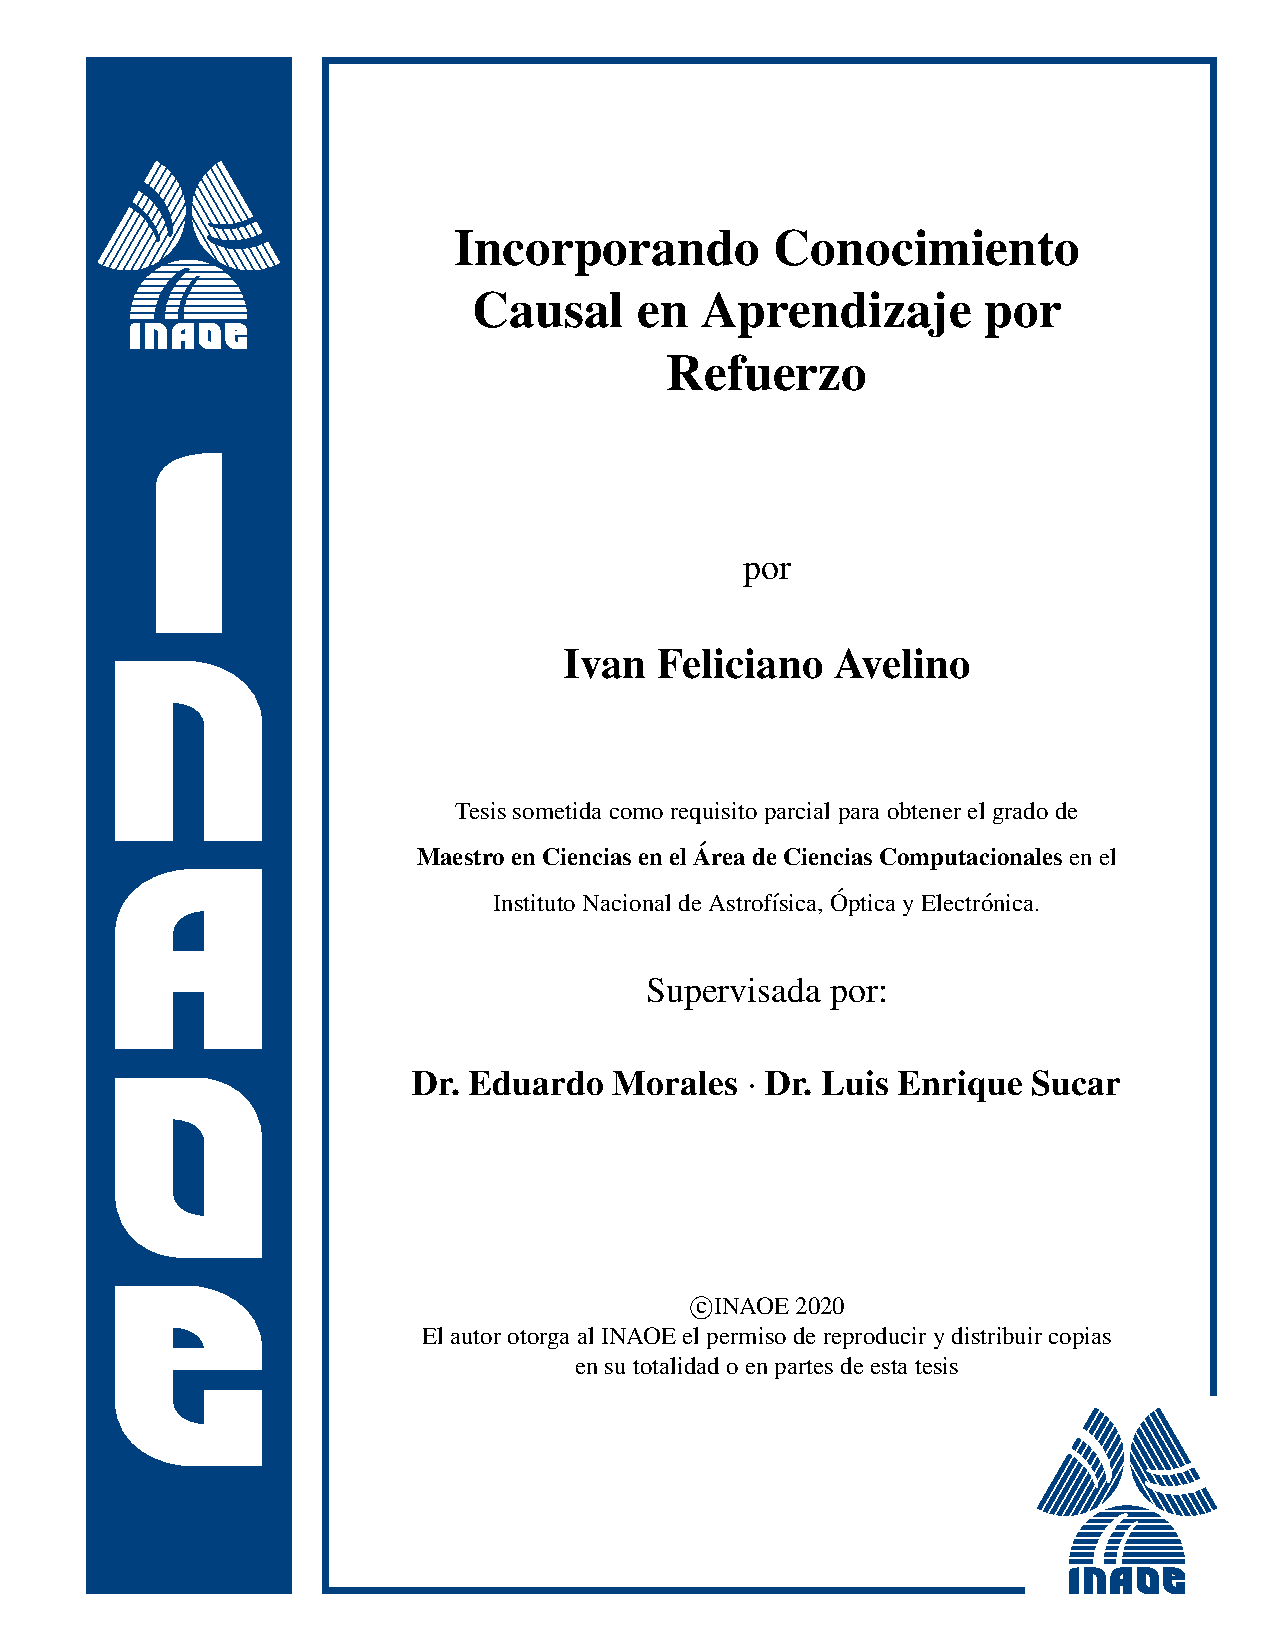
\includepdf[pages={1}]{portada.pdf}
% \frontmatter

% \maketitle

% % ******************************* Thesis Dedidcation ********************************

\begin{dedication} 

I would like to dedicate this thesis to my loving parents \dots

\end{dedication}


% % ******************************* Thesis Declaration ***************************

\begin{declaration}

I hereby declare that except where specific reference is made to the work of 
others, the contents of this dissertation are original and have not been 
submitted in whole or in part for consideration for any other degree or 
qualification in this, or any other university. This dissertation is my own 
work and contains nothing which is the outcome of work done in collaboration 
with others, except as specified in the text and Acknowledgements. This 
dissertation contains fewer than 65,000 words including appendices, 
bibliography, footnotes, tables and equations and has fewer than 150 figures.

% Author and date will be inserted automatically from thesis.tex \author \degreedate

\end{declaration}


% % ************************** Thesis Acknowledgements **************************

\begin{acknowledgements}      


And I would like to acknowledge ...


\end{acknowledgements}

% ************************** Thesis Abstract *****************************
% Use `abstract' as an option in the document class to print only the titlepage and the abstract.
\begin{abstract}
Reinforcement learning and Causal Inference are indispensable part of machine learning. However, they are usually treated separately, although that both are directly relevant to problem solving methods.
One of the challenges that emerge in Reinforcement Learning, is the trade-off between exploration and exploitation. In this work 
we propose to use causal models to attend the learning 
process of an agent. The causal models helps to restrict the search space by reducing the actions that an agent can take through interventional queries like: \textit{Would I have achieved my goal if I had drop the passenger off here?}. This simulates common sense that lightens the time it takes the trial and error approach. We attack the classic taxi problem and we show that using causal models in the Q-learning action selection step leads to higher
and faster jump-start reward and convergence, respectively.
e

e advocate that a good abstract should (1) give a high-level presen-
tation of the subject area studied, (2) reason about the importance and why it is an
interesting area worthy to be studied, (3) present a high-level description of the
approach, and (4) summarise the contribution. An informative abstract should sum-
marise all the major sections of the report, the key concepts, contributions, and
conclusions. A typical abstract is about 250–500 words. This is not more than 10–20
sentences, so you will obviously have to choose your words very carefully in order
to cover so much information in such a condensed format. You must therefore
exclude any general and obvious statements; the phrasing should be concentrated
and compact.
En este trabajo de investigación el objetivo es 
acelerar el entrenamiento de un agente de RL
a través de la selección de acciones guiadas por un 
modelo causal para completar tareas que tienen una
estructura causal subyacente.
En general, un agente comienza su búsqueda a ciegas,
mediante interacciones a prueba y error.
Sin embargo, éste puede, a través de intervenciones
en un modelo causal, hacer consultas del tipo: \textit{¿Qué tal si hago ...?} Estas intervenciones sobre variables 
que describen a las acciones permiten usar al modelo
como ``oráculo'' para no realizar acciones que lleven
a estados no deseados o para no evitar la acción que
lleve a una meta.
Se ha probado que la formulación actual del aprendizaje
por refuerzo no es un problema causal.
Por lo tanto, es una suposición fuerte 
decir que todos los problemas 
en aprendizaje por refuerzo contienen mecanismos causales. 
Sin embargo, hay tareas en las
que un experto o incluso el mismo algoritmo puede
aprender el modelo causal latente.

\end{abstract}


\begin{resumen}


El aprendizaje por refuerzo es un paradigma de aprendizaje por interacción indispensable dentro del aprendizaje automático. Uno de los principales retos que surgen en 
el aprendizaje por refuerzo, es el compromiso entre la 
explotación de la información que ya se conoce o 
exploración del ambiente. Para resolver este problema, 
un agente puede limitar su espacio de búsqueda al 
aprovechar propiedades de su ambiente o utilizar 
conocimiento dado previamente. Específicamente, el agente
puede explotar las relaciones causales de su mundo. En este
trabajo se propone auxiliar el proceso de aprendizaje de
un agente en tareas dirigidas por metas donde la estructura
causal es brindada. 
Un modelo causal ayuda a restringir el espacio de búsqueda, al
guiar la toma de decisiones de un agente, mediante consultas en un grafo causal. Por ejemplo, verificando qué variables 
son causas directas de otras.
Esto parece simular un sentido común que disminuye el
tiempo que toma el enfoque a prueba y error.
Entre las contribuciones de esta investigación están: 1)
la representación de la información extra en un grafo causal y 2) un algoritmo para guiar la selección de acciones 
a través de consultas en el grafo.
Se atacan un par de problemas sobre dominios discretos y continuos que son relativamente pequeños y simples para
probar el concepto propuesto.
Se muestra, a través de diferente experimentos, que
usar información adicional de una estructura causal
en la selección de acciones del algoritmo Q-learning
lleva a una recompensa final y a un salto inicial de
recompensa mayores. Además, se muestra que 
no es obligatorio contar con una estructura causal 
completa y correcta. Incluso, guiar a una agente con una estructura parcial o con relaciones falsas se alcanza un mejor desempeño que no utilizar información suplementaria.

\end{resumen}
% *********************** Adding TOC and List of Figures ***********************

\tableofcontents

% \listoffigures

% \listoftables

% \printnomenclature[space] space can be set as 2em between symbol and description
%\printnomenclature[3em]

% \printnomenclature

% ******************************** Main Matter *********************************
\mainmatter

%!TEX root = ../thesis.tex
%*******************************************************************************
%*********************************** First Chapter *****************************
%*******************************************************************************

\chapter{Introducción}  %Title of the First Chapter

%!TEX root = ../thesis.tex
%*******************************************************************************
%****************************** Second Chapter *********************************
%*******************************************************************************

\chapter{Marco teórico}\label{chapter2}

\graphicspath{{Chapter2/Figs/}}


% {\color{magenta}Aquí debo ahondar más en lo que se plasma en este capítulo. Decir que en RL empezamos desde el planteamiento de MDP, y como se soluciona con RL, monte carlo
% te lleva a TD y eso s Q learning. luego de la versión para ambientes continuos y del estado del arte que es DQN. Por el lado de causalitdad }

En este capítulo se describen algunos conceptos fundamentales para entender
el problema atacado, la propuesta de solución y los métodos que 
se evalúan en los experimentos.
Dado que los dos campos que conducen este trabajo son
el aprendizaje por refuerzo y la causalidad, estos son
presentados de manera general en las siguientes dos
secciones.
La Sección \ref{rl-section} describe lo que es el aprendizaje
por refuerzo, el planteamiento del problema
como un proceso de decisión de Markov, las ecuaciones
fundamentales para su solución y algunos métodos para
resolverlo.
La Sección \ref{causation-section} contiene las ideas que se utilizan
con respecto al enfoque intervencionista de causalidad que se sigue en este trabajo, la definición de causalidad propuesta
por \cite{spirtes2000causation}, la 
representación de conocimiento en modelos gráficos 
causales y la definición de intervenciones en un modelo usando el operador $do(\cdot)$ \cite{pearl_2009}.

\section{Aprendizaje por refuerzo}\label{rl-section}

El aprendizaje por interacción es una idea esencial que subyace en casi todas la teorías
de aprendizaje e inteligencia \cite{sutton_barto_2018}.
Una perspectiva dentro del \textit{aprendizaje automático} \cite{Goodfellow-et-al-2016} enfocada al aprendizaje dirigido a metas a través de interacciones es el \textit{aprendizaje por refuerzo}.

El aprendizaje por refuerzo se encarga de aprender el comportamiento de un agente 
de tal forma que se maximice una señal de recompensa numérica, esto es, a que un
agente aprenda a mapear estados de su mundo a acciones. Al aprendiz o agente no se le 
dice qué acciones tomar, en cambio éste debe descubrir cuáles, al intentarlas, producen
una mayor recompensa. Las dos características más importantes que diferencían al
aprendizaje por refuerzo de otros paradigmas en el aprendizaje automático son 
la búsqueda a prueba-y-error y la recompensa retrasada. Donde que la recompensa sea retrasada significa que el agente debe ser 
capaz de aprender cuales son acciones deseables basándose en una recompensa que puede ocurrir muy en el futuro.

\begin{figure}[h]
    \centering
    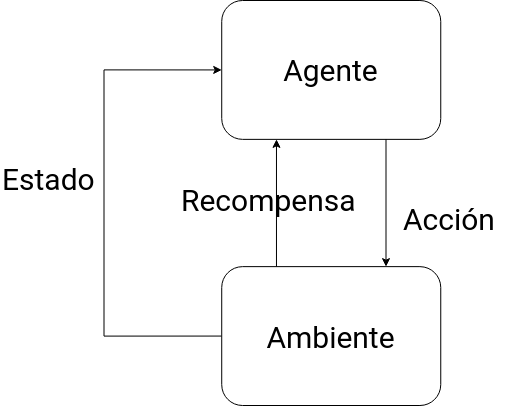
\includegraphics[scale=0.3]{Chapter2/Figs/agend_interaction.png}
    \caption{La idea general del RL es que un agente interactúa con un ambiente para
    aprender a partir de experiencias. Cada paso en el tiempo, el agente se encuentra
    en cierto estado $s\in \mathcal{S}$ y toma la acción $a \in \mathcal{A}$. Como
    resultado, el estado del mundo cambia y recibe una recompensa $r$.}
\end{figure}

En las siguientes secciones primero se formaliza el problema de aprendizaje por refuerzo como
un problema de control óptimo para procesos de decisión de Markov incompletos (MDP por sus siglas en inglés) y luego se
describe el algoritmo \textit{Q-learning}, cuyo desarrollo involucró un gran avance en esta área de la IA  .

\subsection{Procesos de decisión de Markov}


Los procesos de decisión de Markov (MDP) son un marco de trabajo para
definir el problema de aprender
mediante interacciones para 
alcanzar una meta. El tomador de 
decisiones es llamado \textit{agente}.
El agente interactúa con un mundo, que
abarca todo fuera de éste, y se
conoce como \textit{ambiente}.
Estos dos elementos
interactúan continuamente, el agente
selecciona \textit{acciones} y
el ambiente responde a estas 
acciones presentando nuevos 
\textit{estados} al agente. Además,
el ambiente envía \textit{recompensas},
las cuales son valores numéricos 
que el agente busca maximizar con
el paso del tiempo mediante la 
selección de sus acciones.

Formalmente, un MDP es una tupla $< \mathcal{S}, \mathcal{A}, \mathcal{P}, \mathcal{R}, \gamma>$ tal que

\begin{itemize}
    \item $\mathcal{S}$ es el conjunto de estados, donde $s_t$ denota el estado $s\in \mathcal{S}$ al tiempo $t$.
    \item $\mathcal{A}$ es el conjunto de acciones, donde $a_t \in \mathcal{A}$
    denota la acción realizada en un estado $s$ en el tiempo $t$.
    \item $\mathcal{P}_{ss'}^{a}: \mathcal{S}\times \mathcal{A} \times \mathcal{S} \rightarrow [0, 1]$ (también denotada por $\mathcal{P}$) es una función de probabilidad de transición de pasar del estado $s \in \mathcal{S}$ a $s' \in \mathcal{S}$ cuando se toma la acción $a$.% en el tiempo $t$.
    \item $\mathcal{R}_{ss'}^{a}: \mathcal{S} \times \mathcal{A} \times \mathcal{S} \rightarrow \mathbb{R}$ (también denotada por $\mathcal{R}$) es la función de recompensa inmediata que el agente recibe depués de pasar del $s$ a $s'$.
    \item $\gamma \in [0,1]$ es el factor de descuento que sirve para
    calcular el retorno esperado con descuento.
\end{itemize}


Además de estos componentes, un sistema de aprendizaje por refuerzo subsume otros elementos como: una \textit{política} y una \textit{función de valor}. Una política es una función $\pi$ que mapea estados
a acciones y que maximiza alguna medida de refuerzo a largo plazo. Mientras que la recompensa expresa lo que es bueno
de manera inmediata, una función de valor especifica lo que
es bueno a la larga. 
%Un modelo consiste del conocimiento de la
%función de probabilidad de transición $\mathcal{P}$ y
%de la función de recompensa $\mathcal{R}$.
El aprendizaje por refuerzo aprende las funciones de valor o la política mientras 
interactúa con el ambiente.
% %  
% % Whereas the reward signal indicates what is good in an immediate sense, a value
% % function specifies what is good in the long run. Roughly speaking, the value of a state is the total amount of reward an agent can expect to accumulate over the future, starting from that state.

% % Es la recompensa total que un agente puedeesperar acumular empezando en un estados(V(s)) oen un estado haciendo una acona(Q(s,a))

% % 

% % element of some reinforcement learning systems is a model of
% % the environment. This is something that mimics the behavior of the environment, or more generally, that allows inferences to be made about how the environment will behave.
 Un paso en la interacción de un agente con el ambiente se puede ver como que dado un estado $s_t \in \mathcal{S}$ y un
acción $a_t\in \mathcal{A}$, el agente pasa a un nuevo
estado $s_{t+1} \in \mathcal{S}$ y recibe una recompensa
$r_{t+1}$.
% Una política $\pi$ es una función de los estados percibidos del ambiente a acciones que se toman cuando se está en esos estados ($\pi : \mathcal{S} \rightarrow \mathcal{A}$).
% El problema fundamental en los MDP es
% encontrar una política óptima; esto es, 
% aquella que maximiza la recompensa esperada por el agente a largo plazo.
En RL, la meta del agente está formalizada
en términos de la señal de recompensa que
envía el ambiente al agente. En cada paso $t$, la recompensa es un número real $r_t \in \mathbb{R}$. La meta de un agente
es maximizar la recompensa total recibida.
Esto significa, que no solo se maximiza la recompensa inmediata sino la recompensa acumulada a largo plazo.

En general, se busca maximizar el \textit{retorno
esperado}, donde el retorno, denotado por $R_t$, se define como alguna función de la secuencia de recompensas. 
El \textit{retorno esperado con descuento} es la suma acumulada de recompensas futuras. El factor de descuento $\gamma$
define que tantas recompensas en el 
futuro son consideradas. Si $\gamma = 0$
solo la recompensa inmediata es
tomada en cuenta.

\[
R_t = r_{t+1} + \gamma r_{t+2} + \gamma^2 r_{t+3} + \gamma^3 r_{t+4} + \dots = 
\sum_{k = 0}^\infty \gamma^{k} r_{t+k+1}
\]

Si se tiene un punto terminal se llaman tareas \textit{episódicas}, si no se tiene se conocen como tareas \textit{continuas}.

% \subsection{Política y funciones de valor}

Una política, denotada por $\pi(s, a)$, describe una manera de actuar. Es una función que mapea un estado $s$ y una acción $a$ a la probabilidad de tomar esa acción en ese estado.
Por lo tanto para un estado dado, 
$\sum_a \pi (s, a) = 1$. El problema fundamental en los MDP es encontrar una política óptima $\pi^*$, es decir, aquella que maximiza la recompensa que espera recibir el agente a largo plazo.
A veces es escrita como $\pi^*(s) = a$, el cual es un mapeo de estado a las acciones óptimas en esos estados.

Para aprender la política óptima, se utilizan las \textit{funciones de valor}. Existen dos tipos de funciones de valor: la \textit{ función de valor de estado},
denotada por $V(s)$, y la \textit{función de valor de acción}, expresada como $Q(s, a)$.

La función de valor de estado describe el valor de un estado al seguir una política. Es el retorno esperado partiendo del estado $s$, actuando de acuerdo
a la política $\pi$

\begin{equation}\label{eq:state-value-func}
V^\pi(s) = \mathbb{E}_\pi[R_t | s_t = s].    
\end{equation}


La función de valor no necesariamente es la misma para dos políticas diferentes
en un mismo ambiente. Esto es porque el valor del estado
cambia dependiendo del comportamiento del agente, ya que la manera de actuar
en un estado en particular afecta cuánta recompensa se espera recibir.
La razón de usar el valor esperado  es porque existe aleatoriedad en lo que
sucede después de llegar a un estado. Se puede contar con una política estocástica, lo que significa que se necesitan combinar los resultados de 
todas las acciones que se toman. Además, la función de transición puede ser estocástica, lo cual implica cierta incertidumbre de llegar a cualquier 
estado.

La otra función de valor que se utiliza es la función de valor de acción.
La función de valor de acción define el valor de 
tomar una acción en algún estado cuando se sigue cierta política. Es el
retorno esperado dados un estado y una acción bajo la política $\pi$

\begin{equation}\label{eq:action-value-func}
Q^\pi (s,a) = \mathbb{E}[R_t | s_t = s, a_t = a].    
\end{equation}

Las funciones de valor óptimas se definen como
\[
V^*(s) = \max_{\pi} V^\pi(s) \text{ y } Q^*(s, a) = \max_{\pi} Q^\pi (s,a).
\]


Las funciones anteriores pueden ser expresadas mediante las ecuaciones de optimalidad de Bellman \cite{bellman1966dynamic}.
Las ecuaciones de Bellman están presentes en casi todos lo métodos de RL y es importante conocer de donde surgen para comprender estos algoritmos. Por lo tanto, a continuación se muestra la obtención de las ecuaciones
de Bellman como lo muestra \cite{greaves}.

Las funciones $\mathcal{P}_{ss'}^a$ y $\mathcal{R}_{ss'}^a$ son la probabilidad de transición y la recompensa esperada, respectivamente. La primera se define como
$\mathcal{P}_{ss'}^a = P(s_{t+1} = s' | s_t = s, a_t = a)$,
y la segunda como
$\mathcal{R}_{ss'}^a = \mathbb{E}[r_{t+1} | s_t = s, s_{t+1} = s', a_t = a]$.

Usando la función de retorno esperado con descuento, se puede
reescribir la ecuación \ref{eq:state-value-func} como

\[
V^\pi(s) = \mathbb{E}_\pi[r_{t+1} + \gamma r_{t+2} + \dots | s_t = s] = \mathbb{E}_{\pi}[\sum_{k = 0}^\infty \gamma^{k} r_{t+k+1} | s_t =s].
\]


Si se deja fuera de la suma la primera recompensa, se tiene
\[
V^\pi(s) = \mathbb{E}_\pi[r_{t+1} + \gamma \sum_{k = 0}^\infty \gamma^{k} r_{t+k+2} | s_t =s].
\]

El valor esperado describe el retorno esperado que se obtiene si se parte del estado $s$ siguiendo la política $\pi$.
El valor esperado puede ser escrito explícitamente mediante la suma de todas
las acciones posible y todos los posible estados, por lo tanto se tienen las siguientes ecuaciones

\[
\begin{split}
\mathrm{E}_\pi[r_{t+1}| s_t=s] &= \sum_a \pi(s,a) \sum_{s'}\mathcal{P}_{ss'}^a\mathcal{R}_{ss'}^a,\\
\mathbb{E}_\pi[\gamma \sum_{k = 0}^\infty \gamma^{k} r_{t+k+2} | s_t =s] &=
\sum_a \pi(s,a) \sum_{s'}\mathcal{P}_{ss'}^a \gamma \mathbb{E}_\pi[\sum_{k = 0}^\infty \gamma^{k} r_{t+k+2} | s_{t+1} = s']
\end{split}.
\]

Con las ecuaciones anteriores se puede reescribir $V^\pi(s)$ de la
siguiente forma
\[
V^\pi(s) = \sum_a \pi(s,a) \sum_{s'}\mathcal{P}_{ss'}^a [\mathcal{R}_{ss'}^a +
\gamma \mathbb{E}_\pi[\sum_{k = 0}^\infty \gamma^{k} r_{t+k+2} | s_{t+1} = s']].
\]

La última parte de la ecuación tiene
la misma forma que la ecuación \ref{eq:state-value-func}, por lo tanto, sustituyéndola, se tiene

\begin{equation}\label{eq:bellman-state-val}
    V^\pi(s) = \sum_a \pi(s,a) \sum_{s'}\mathcal{P}_{ss'}^a [\mathcal{R}_{ss'}^a + \gamma V^\pi(s')].
\end{equation}

La ecuación de Bellman para la función de valor de acción se deriva de la misma manera.

\begin{equation}\label{eq:bellman-acion-val}
    Q^\pi(s, a) = \sum_{s'}\mathcal{P}_{ss'}^a [\mathcal{R}_{ss'}^a + \gamma \pi(s',a')Q^\pi(s', a')].
\end{equation}

Las ecuaciones de Bellman permiten expresar valores de estados como
valores de otros estados, es decir, si se conoce el valor de $s_{t+1}$, se puede calcular $s_t$. A partir de las ecuaciones \ref{eq:bellman-state-val} y \ref{eq:bellman-acion-val} los valores óptimos de
las funciones de valor quedan como sigue

\[
V^*(s) = \max_{a}\sum_{s'}\mathcal{P}_{ss'}^a[\mathcal{R}_{ss'}^a + \gamma V^*(s')]
\]
y 
\[
Q^*(s,a) = \sum_{s'}\mathcal{P}_{ss'}^a[\mathcal{R}_{ss'}^a + \gamma \max_{a'}Q^*(s',a')].
\]

Un MDP busca la solución a las ecuaciones de Bellman, lo que equivale a encontrar
la política óptima. Si $\mathcal{P}$ y $\mathcal{R}$ son conocidas, i.e., el
modelo es conocido un MDP se puede resolver mediante programación dinámica o
programación lineal. En caso contrario, cuando el modelo no es conocido,
se utiliza aprendizaje por refuerzo.
% Una política $\pi$ es una función de los estados percibidos del ambiente a acciones que se toman cuando se está en esos estados ($\pi : \mathcal{S} \rightarrow A$). 
% Whereas the reward signal indicates what is good in an immediate sense, a value
% function specifies what is good in the long run. Roughly speaking, the value of a state is the total amount of reward an agent can expect to accumulate over the future, starting from that state.

\subsection{Método Monte Carlo}\label{subsection-montecarlo}

El método Monte Carlo es un enfoque que busca resolver problemas
de aprendizaje por refuerzo con tareas episódicas, donde 
no existe un modelo del ambiente. 
Es un método iterativo y converge a la política
al incrementar el número de episodios.

Existe una tabla $Q$ que almacena el valor de acción para cada posible
par de estado-acción. El valor es el promedio sobre
todos los retornos, que han sido obtenidos durante todos los episodios. 
Un elemento de la tabla es actualizado cada vez que un par estado-acción
es visitado por el agente. La ecuación de actualización se muestra en la 
siguiente ecuación, donde $N(s_t, a_t)$ es el número de visitas al 
par estado-acción $(s_t, a_t)$.

\[
Q(s_t, a_t) = Q(s_t, a_t) + \frac{1}{N(s_t, a_t)} (R_t - Q(s_t, a_t)).
\]

Los diferentes retornos pueden 
ser ponderados por un peso $\alpha$.
En vez de tomar el promedio
verdadero, retornos recientes pueden tener un peso mayor o menor

\begin{equation}\label{eq:montecarlo-update}
\begin{split}
Q(s_t, a_t) &= Q(s_t, a_t) + \alpha(R_t - Q(s_t, a_t))\\
&= (1-\alpha)Q(s_t, a_t) + \alpha R_t.
\end{split}
\end{equation}

El método Monte Carlo itera sobre episodios. Durante el paso de evaluación, el 
agente actúa de acuerdo a la política $\pi$ de un episodio. Cuando el 
episodio se termina, el agente recolecta una secuencia de experiencia $s_1, a_1, r_1, s_2, \dots, s_t$ y puede actualizar la tabla $Q$ de acuerdo
con ésta.
Para cada par estado-acción en la secuencia, se obtiene el retorno 
esperado $R_t$ y se actualiza el elemento correspondiente en la tabla $Q$ 
de acuerdo con la ecuación \ref{eq:montecarlo-update}.
Durante el paso de mejora,  la
política $\pi$ se actualiza de acuerdo a la tabla $Q$. En la siguiente iteración,
el paso de evaluación se realiza con la política nueva que sea obtiene de la
actualización.

Normalmente, la política de actualización básica es una política voraz. El agente
siempre elige la acción con el máximo valor de acción. Sin embargo, explotar la acciones vorazmente con el conocimiento actual puede conducir a que el
agente quede atascado en una política no óptima. Para evitar 
este caso, acciones exploratorias deben tomarse en cuenta de vez en cuando.
Una política es llamada $\epsilon$-greedy, si la mejor acción actual se toma 
con una probabilidad de $1-\epsilon$ y una acción aleatoria se toma con una 
probabilidad $\epsilon$. La ecuación de la política $\epsilon$-greedy
se puede definir de la siguiente manera

\[
\pi(s,a) = 
   \begin{cases} 
      1 - \epsilon + \frac{\epsilon}{|\mathcal{A}|} & \mbox{si } a= 
      \argmax_{a \in \mathcal{A}} 
      Q(s,a)   \\
      \frac{\epsilon}{|\mathcal{A}|} & \mbox{ en otro caso }
   \end{cases}
\]

$\epsilon$ es un valor entre 0 y 1 y pondera la relación entre
exploración y explotación.

\subsection{Métodos de diferencias temporales}

Una idea central e importante en RL es el aprendizaje 
a través de diferencias temporales (TD por sus siglas en inglés).
El aprendizaje TD es una combinación de ideas del método Monte Carlo y programación dinámica. 
% Los métodos de diferencias 
% temporales pueden aprender de experiencia sin 
% un modelo del ambiente como en los Monte Carlo. Por otro lado, 
% al igual que en programación dinámica,
% las actualizaciones de los métodos TD se basan en otros 
% estimados aprendidos, sin esperar a una salida final.
La ventaja de los métodos TD es que se pueden aplicar tareas de aprendizaje por refuerzo en línea y continuas.
La política se actualiza cada paso de tiempo $t$ por lo que no se necesitan
episodios completos (como en programación dinámica). Además, no se requiere ningún modelo del ambiente (igual que en el método Monte Carlo). 

En los métodos TD, el retorno esperado verdadero $R_t$ no está disponible
y es aproximado con un valor TD-target. El TD-target se determina con la suma de la recompensa inmediata y el valor esperando con descuento del 
siguiente estado $r_{t+1} + \gamma V(s_{t+1})$. 

\begin{algorithm}[H]
  	\caption{Algoritmo general de los métodos TD}
	\label{alg:TD-algo}
  \begin{algorithmic}[1]
  \setstretch{1}
  \REQUIRE La política $\pi$ a ser evaluada, $\alpha \in (0,1]$.
  \STATE Inicializar arbitrariamente $V(s)$, para todo $s\in \mathcal{S}$ excepto donde $V(terminal) = 0$.
  
  \FOR{$episodio = 1, \dots, M$}
    \STATE Inicializar $s_0$.
    \FOR{$t = 0, \dots, T$}
    \STATE $a_{t} \leftarrow$ acción dada por $\pi$ para $s_t$.
    \STATE Tomar acción $a_t$ y observar $r_{t+1}, s_{t+1}$.
    \STATE $V(s_t) \leftarrow V(s_t) + \alpha\underbrace{[\underbrace{r_{t+1} + \gamma V(s_{t+1})}_{TD-target} - V(s_t)]}_{TD-error}$.
    \STATE $s_t \leftarrow s_{t+1}$.
    \ENDFOR
  \ENDFOR
  \end{algorithmic}
\end{algorithm}



% \RestyleAlgo{boxruled}
% \begin{algorithm}[!hbt]
% 	\caption{Algoritmo general de los métodos TD}
% 	\label{alg:TD-algo}
	
	
% 	\SetAlgoLined\DontPrintSemicolon
%     \SetAlgoHangIndent{0.5em}
% 	%\scriptsize
% 	\SetAlFnt{\large} 
%     \SetKwData{patterns}{\textit{PS}}
% 	\SetKwInOut{Input}{Entrada}
	
% 	\Input{La política $\pi$ a ser evaluada, $\alpha \in (0,1]$.}
% 	\BlankLine
	
%     Inicializar arbitrariamente $V(s)$, para todo $s\in \mathcal{S}$ excepto donde $V(terminal) = 0$\;
% 	Repetir por cada episodio:\;
% 	\hspace{0.5cm}Inicializar $s_t$\;
% 	\hspace{0.5cm}Repetir por cada paso del episodio:\;
% 	\hspace{1cm}$a_t \leftarrow$ acción dada por $\pi$ para $s_t$\;
% 	\hspace{1cm}Tomar acción $a_t$, observar $r_{t+1}$, $s_{t+1}$\;
% 	\hspace{1cm}$V(s_t) \leftarrow V(s_t) + \alpha\underbrace{[\underbrace{r_{t+1} + \gamma V(s_{t+1})}_{TD-target} - V(s_t)]}_{TD-error}$\;
%     \hspace{1cm}$s_t \leftarrow s_{t+1}$\;
%     \hspace{0.5cm}hasta que $s_t$ sea terminal o inválido\;
% \end{algorithm}

% \subsection{Aprendizaje por refuerzo profundo}
% \subsubsection{Deep Q Network}

El algoritmo $Q$-learning \cite{watkins1992q} es un método de control TD \textit{fuera de política}, es decir,
la política $\pi$ no se utiliza para actualizar la tabla $Q$. 
La regla de actualización del $Q$-learning está dada por 

\[
Q(s_t, a_t) \leftarrow Q(s_t, a_t) + \alpha[r_{t+1} + \gamma \max_a Q(s_{t+1}, a) - Q(s_t, a_t)]
\]

\begin{algorithm}[H]
  	\caption{Algoritmo $Q$-learning}
	\label{alg:q-algo}
  \begin{algorithmic}[1]
  \setstretch{1}
  \REQUIRE $\alpha \in (0,1]$, $\epsilon \in (0, 1]$.
  \STATE Inicializar arbitrariamente $Q(s,a)$, para todo $s\in \mathcal{S}$ excepto donde $Q(terminal, \cdot) = 0$.
  
  \FOR{$episodio = 1, \dots, M$}
    \STATE Inicializar $s_0$.
    \FOR{$t = 0, \dots, T$}
    \STATE Elegir $a_t$ usando una política derivada de $Q$ (e.g., $\epsilon$-greedy).
    \STATE Tomar acción $a_t$ y observar $r_{t+1}, s_{t+1}$.
    \STATE $Q(s_t, a_t) \leftarrow Q(s_t, a_t) + \alpha [r_{t+1} + \gamma \max_a Q(s_{t+1}, a) - Q(s_t, a_t)]$.
    \STATE $s_t \leftarrow s_{t+1}$.
    \ENDFOR
  \ENDFOR
  \end{algorithmic}
\end{algorithm}

% \RestyleAlgo{boxruled}
% \begin{algorithm}[!hbt]
% 	\caption{Algoritmo $Q$-learning}
% 	\label{alg:q-algo}
	
	
% 	\SetAlgoLined\DontPrintSemicolon
%     \SetAlgoHangIndent{0.5em}
% 	%\scriptsize
% 	\SetAlFnt{\large} 
%     \SetKwData{patterns}{\textit{PS}}
% 	\SetKwInOut{Input}{Entrada}
	
% 	\Input{$\alpha \in (0,1]$, $\epsilon \in (0, 1]$}
% 	\BlankLine
	
%     Inicializar arbitrariamente $Q(s,a)$, para todo $s\in \mathcal{S}$ excepto donde $Q(terminal, \cdot) = 0$\;
% 	Repetir por cada episodio:\;
% 	\hspace{0.5cm}Inicializar $s_t$\;
% 	\hspace{0.5cm}Repetir por cada paso del episodio:\;
% 	\hspace{1cm}Elegir $a_t$ usando una política derivada de $Q$ (e.g., $\epsilon$-greedy)\;
% 	\hspace{1cm}Tomar acción $a_t$, observar $r_{t+1}$, $s_{t+1}$\;
% 	\hspace{1cm}$Q(s_t, a_t) \leftarrow Q(s_t, a_t) + \alpha [r_{t+1} + \gamma \max_a Q(s_{t+1}, a) - Q(s_t, a_t)]$\;
%     \hspace{1cm}$s_t \leftarrow s_{t+1}$\;
%     \hspace{0.5cm}hasta que $s_t$ sea terminal o inválido\;
% \end{algorithm}

\subsection{Q-learning profundo}

A pesar de que el algoritmo Q-learning resuelve muchos problemas, 
le es difícil hacer frente a situaciones donde el tamaño del conjunto de estados
es muy grande. Por ejemplo, en algunos videojuegos se puede tener una gran variedad
de imágenes diferentes, por lo que  si se decide a usar pixeles como 
estados individuales es fácil notar que se tiene que seguir la pista de muchos
estados y se tienen que aproximar muchos valores. 
Una solución a este problema es usar una representación no lineal que mapea 
el par estado-acción a un valor.
Existen diversas formas de representar y entrenar dicha función, la que 
se explora en esta sección es usando una red neuronal profunda \cite{lapan_2020, Goodfellow-et-al-2016}.

Los autores en \cite{mnih2013playing} adaptaron el método Q-learning 
para que éste aproveche el uso de redes neuronales profundas como aproximadores
de funciones no lineales y un \textit{búfer de repetición} para estabilizar 
el aprendizaje. Este método es conocido como Q-learning profundo o Red Q profunda (DQN por sus siglas en inglés).
La primera versión del algoritmo DQN fue aplicada al dominio de los videojuegos de Atari \cite{bellemare2013arcade}. De manera muy general, la red profunda recibe como entrada un conjunto de fotogramas a escala de grises de un videojuego, que son procesados por varias capas convolucionales para
extraer características del espacio y tiempo. El último mapa de características
de las capas convolucionales es procesado por varias capas completamente conectadas, que codifican los efectos de las acciones.

Son tres los elementos que forman las bases que permitieron demostrar
la eficiencia y efectividad de este enfoque en ambientes complejos: el uso de una política $\epsilon$-greedy, un búfer de repetición o experiencia de repetición \cite{lin1993reinforcement} y una red objetivo.
El búfer cíclico de experiencias de repetición guarda transiciones de la forma 
$(s_t, a_t, s_{t+1}, r_{t+1})$, permitiendo que un agente de RL 
tome muestras de éste y entrene sobre datos previamente observados. 
Esto no solo reduce la cantidad de interacciones necesarias con el ambiente,
también permite obtener lotes de muestras, reduciendo la varianza de 
las actualizaciones de aprendizaje. Además, al tomar muestras de una memoria
muy grande, se rompen las correlaciones temporales que pueden afectar negativamente al algoritmo de RL.
El segundo método importante es el uso de una red objetivo que inicialmente contiene los pesos de la red que representa la política, sin embargo se mantiene
fija por un periodo largo de tiempo.
En vez de tener que calcular el error TD basándose en los estimados
oscilantes de los valores Q, la red de la política usa la red objetivo fija.
Durante el entrenamiento, los pesos de la red objetivo son actualizados 
para coincidir con la red de la política después de un número establecido de pasos.



\begin{algorithm}[H]
  	\caption{Algoritmo $Q$-learning profundo con experiencias de repetición}
	\label{alg:dqn-algo}
  \begin{algorithmic}[1]
  \setstretch{1}
  \STATE Inicializar búfer de experiencias $D$ a una capacidad $N$.
  \STATE Inicializar la función de valor de acción $Q$ con pesos aleatorios $\theta$.
  \STATE Inicializar la función de valor de acción objetivo $\hat{Q}$ con pesos $\theta^- = \theta$.
  
  \FOR{$episodio = 1, \dots, M$}
    \STATE Inicializar secuencia $s_1 = {x_1}$ y preprocesar secuencia $\phi_1 = \phi(s_1)$.
    \FOR{$t = 0, \dots, T$}
    \STATE Elegir $a_t$ usando una política $\epsilon$-greedy.
    \STATE Tomar acción $a_t$, observar recompensa $r_{t}$ e imagen $x_{t+1}$.
    \STATE Asignar $s_{t+1} =  s_t, a_t, x_{t+1}$ y preprocesar $\phi_{t+1} = \phi(s_{t+1})$.
    \STATE Guardar transición $(\phi_t, a_t, r_t, \phi_{t+1})$ en $D$.
    \STATE De $D$ tomar una muestra aleatoria de un lote de transiciones $(\phi_j, a_j, r_j, \phi_{j+1})$.
    \STATE Establecer
	\[
	 y_j = 
   \begin{cases} 
      r_j  & \mbox{si el episodio termina en el paso } j + 1 \\
      r_j + \gamma \max_{a'}\hat{Q}(\phi_{j+1}, a'; \theta^-) & \mbox{en cualquier otro caso.}
   \end{cases}
	\]
	\STATE Realizar el paso del
	descenso de gradiente sobre $(y_j -  Q(\phi_j,a_j;\theta))^2$ con respecto a los parámetros de la red $\theta$.
	\STATE Cada $C$ pasos reiniciar $\hat{Q} = Q$.
    \ENDFOR
  \ENDFOR
  \end{algorithmic}
\end{algorithm}

% \RestyleAlgo{boxruled}
% \begin{algorithm}[!hbt]
% 	\caption{Algoritmo $Q$-learning profundo con experiencias de repetición}
% 	\label{alg:dqn-algo}
	
% 	\SetAlgoLined\DontPrintSemicolon
%     \SetAlgoHangIndent{0.5em}
% 	%\scriptsize
% 	\SetAlFnt{\large} 
%     \SetKwData{patterns}{\textit{PS}}
	
%     Inicializar búfer de experiencias $D$ a una capacidad $N$\;
%     Inicializar la función de valor de acción $Q$ con pesos aleatorios $\theta$\;
%     Inicializar la función de valor de acción objetivo $\hat{Q}$ con pesos $\theta^- = \theta$\;
% 	Repetir por cada episodio:\;
% 	\hspace{0.5cm}Inicializar secuencia $s_1 = {x_1}$ y preprocesar secuencia $\phi_1 = \phi(s_1)$\;
% 	\hspace{0.5cm}Repetir por cada paso del episodio:\;
% 	\hspace{1cm}Elegir $a_t$ usando una política $\epsilon$-greedy\;
% 	\hspace{1cm}Tomar acción $a_t$, observar recompensa $r_{t}$ e imagen $x_{t+1}$\;
% 	\hspace{1cm}Asignar $s_{t+1} = s_t, a_t, x_{t+1}$ y preprocesar $\phi_{t+1} = \phi(s_{t+1})$\;
% 	\hspace{1cm}Guardar transición $(\phi_t, a_t, r_t, \phi_{t+1})$ en $D$\;
% 	\hspace{1cm}A partir de $D$, De $D$ tomar una muestra aleatoria de un lote de transiciones $(\phi_j, a_j, r_j, \phi_{j+1})$\;
% 	\hspace{1cm}Establecer
% 	\[
% 	 y_j = 
%   \begin{cases} 
%       r_j  & \mbox{si el episodio termina en el paso } j + 1 \\
%       r_j + \gamma \max_{a'}\hat{Q}(\phi_{j+1}, a'; \theta^-) & \mbox{en cualquier otro caso.}
%   \end{cases}
% 	\]\;
% 	\hspace{1cm}Realizar el paso del
% 	descenso de gradiente sobre $(y_j -  Q(\phi_j,a_j;\theta))^2$ con respecto a los parámetros de la red $\theta$\;
%     \hspace{1cm}Cada $C$ pasos reiniciar $\hat{Q} = Q$\;
% \end{algorithm}


\newpage
\section{Causalidad}\label{causation-section}


En este trabajo se sigue la interpretación de causalidad  
\textit{intervencionista} según como la han descrito en \cite{woodward2005making, spirtes2000causation, pearl_2009}.
De acuerdo con \cite{pearl2018bookofwhy} existen tres niveles
de razonamiento causal: \textit{observar}, \textit{intervenir}
e \textit{imaginar}.
En el primer nivel, el de asociación, se buscan regularidades
en el ambiente a partir de observaciones. 
En general, se dice que un evento está asociado a otro si observar uno
cambia la probabilidad de observar al otro.
El segundo nivel, intervenir, implica predecir los 
efectos de alteraciones arbitrarias sobre el ambiente
y producir una salida deseada después de elegir entre esas alteraciones. Las intervenciones ocupan un lugar más alto que las
asociaciones porque involucran
no solo observar sino cambiar lo que es.
En el tercer nivel se encuentra
el razonamiento \textit{contrafactual} donde la retrospección
e imaginación permite responde preguntas como ¿por qué?
y ¿qué hubiera pasado si una intervención se hubiera hecho 
en vez de otra?
La parte central del razonamiento causal se encuentra en el segundo
y tercer nivel, donde se puede observar qué pasa después de que 
alguna variable ha sido manipulada o intervenida y donde se puede
preguntar qué hubiera pasado si cierta intervención se hubiera 
hecho de otra forma.

Las relaciones asociativas están basadas en correlaciones
entre eventos o patrones de ocurrencia encontrados en los
datos \cite{pearl2018bookofwhy}. Por otro lado, las relaciones
causales están basadas en patrones de causa-efecto,
los cuales resultan de mecanismos arraigados a la naturaleza
de los eventos observados y que pueden ser obtenidos de 
manipulaciones \cite{sep-causal-models}.

Numerosas técnicas han sido desarrolladas para representar
sistemas de relaciones causales y para inferir 
relaciones causales a partir de probabilidades.
Al conjunto de teorías que buscan caracterizar las
relaciones causa y efecto usando herramientas de la
teoría de probabilidad se le llama \textit{causalidad probabilista}. 
La idea central detrás de estas teorías es que las causas cambian las probabilidades de sus efectos.

El nombre de \textit{modelado causal} se usa para describir al campo 
que estudia los métodos de la \textit{inferencia causal}. Dentro de este campo
entre los autores principales están \cite{pearl2010introduction, spirtes2000causation}, entre otros. En las siguientes secciones
se describen formalmentes algunos elementos importantes utilizados en esta investigación
siguiendo el marco de trabajo de los \textit{modelos gráficos causales} propuesto por esos autores.

De acuerdo con \cite{spirtes2000causation} se entiende a la causalidad 
como una relación entre eventos: \textit{algo sucede y causa que algo más suceda}. Cada causa es un evento específico y cada efecto es una evento
en particular. Asumimos que esta relación es \textit{transitiva}, \textit{irreflexiva} y \textit{antisimétrica}. Esto es 
\begin{enumerate}
    \item Si $A$ es una causa de $B$ y $B$ es una causa de $C$, entonces
    $A$ es también una causa de $C$.
    \item Un evento $A$ no puede causarse a sí mismo.
    \item Si $A$ es una causa de $B$, entonces $B$ no es causa de $A$.
\end{enumerate}

\subsection{Estructura y modelo causal}

Supóngase un conjunto de variables $\mathcal{V}$ que incluyen a $A$ y $X$. 
Se dice que $A$ es causa directa de $X$ con respecto a $\mathcal{V}$
solo en caso de que $A$ sea un miembro de algún conjunto 
$\mathcal{A} \subseteq \mathcal{V} - \{X\}$ tal que 

\begin{itemize}
    \item las variables en $\mathcal{A}$ son causas de $X$,
    \item si las variables en $\mathcal{A}$ llegaran a ocurrir,
    causarían $X$ sin importar si los elementos de $\mathcal{V} - \{X \cup \mathcal{A}\}$ ocurrieran o no,
    \item ningún subconjunto propio de $\mathcal{A}$ satisface
    1) y 2).
\end{itemize}

Una \textit{estructura causal} es un par ordenado $<\mathcal{V}, E>$, donde
$\mathcal{V}$ es un conjunto de variables y $E$ es un conjunto
de pares ordenados de $\mathcal{V}$, donde $<X, Y> \in E$ si
y sólo si $X$ es causa directa de $Y$ con respecto a  
$\mathcal{V}$ \cite{spirtes2000causation}.

Una estructura causal se puede representar como un grafo
dirigido $D = <\mathcal{V},E>$ que representa una estructura causal suficiente $C$ (i.e., que todas las causas de las variables están dentro del conjunto de variables de $C$), donde los vértices de $D$ denotan las variables en $C$ y existe una
arista dirigida de $A$ a $B$ en $D$ si y sólo si $A$ es
una causa directa de $B$.
A un grafo acíclico dirigido que representa una estructura causal se le llama \textit{grafo causal}.

Las aristas de un grafo causal implican una semántica causal: si existe un camino dirigido de $A$ a $X$, entonces $A$ es un una \textit{causa potencial} de $X$. Los caminos dirigidos también se conocen como \textit{caminos causales}. El efecto causal de $A$ sobre $X$ se puede ver como la distribución condicional de $X$ dado $A$ restringida solo a caminos causales \cite{dasgupta2019causal}.

De acuerdo con \cite{pearl_2009}, la estructura causal $D$ de un conjunto de variables $\mathcal{V}$ es un grafo acíclico dirigido (DAG por sus siglas en inglés) en el cual cada nodo corresponde a un elemento distinto de $\mathcal{V}$ y cada arista define una relación funcional directa entre las
variables correspondientes. 

Hay tres condiciones que conectan probabilidades con
grafos causales: \textit{la condición causal de Markov}, \textit{la condición de minimalidad} y \textit{la condición
de fidelidad} \cite{gonzalez-soto, spirtes2000causation}.

\begin{itemize}
    \item \textit{Condición de Markov}. Una variable $V$ o nodo
    en $D$ es independiente de cualquier otra variable $A$ tal que
    $A$ no es ni una causa o efecto de $V$ dadas las causas de $V$.
    \item \textit{Condición de minimalidad}. Ningún subgrafo propio de $D$ satisface la condición causal de Markov.
    \item \textit{Condición de fidelidad}. La condición causal de Markov contiene todas las condiciones de independencia expresadas en el grafo $D$.
\end{itemize}
% Markov Causality: an eventV(or node inG) is independent of every other eventAsuchthatAisn’t either a cause nor an effect ofVgiven the causes ofV.•Causal Minimality: No proper sub-graph ofGsatisfies the Markov Causality condition.•Causal Faithfulness: The Markov Causal condition contains all of the conditional inde-pendence statements expressed by the DAGG

De manera general, un modelo causal de acuerdo con \cite{pearl_2009}, se define como un par $\mathcal{M} = <D, \Theta_D>$ donde $D$
es una estructura causal 
$D$ y un conjunto de 
parámetros $\Theta_D$ compatibles con $D$. Los 
parámetros $\Theta_D$ asignan una función $x_i = f_i (pa_i, u_i)$ a cada $X_i \in\mathcal{V}$
y una medida de  probabilidad  $P(u_i)$ para cada $u_i$, donde $PA_i$ son 
los padres de $X_i$ en $D$ y cada $U_i$ es una perturbación aleatoria distribuida
de acuerdo a $P(u_i)$, independiente de todas las otras $u$.
% \begin{itemize}
%     \item Definición de causalidad.
%     \item El por qué de los modelos causales, ventajas sobre enfoques asociativos
%     \item Escalera de la causalidad
%     \item Definición de causalidad según Pearl y  Spirtes
    
%     \item Conexión entre grafos y probabilidades
%     \item Modelos gráficos causales
%     \item Intervenciones y efectos 
%     \item Obtención de DAG
% \end{itemize}
% he termcausalityisdefined in terms of common language and then the mathematical machinery required to modelcausality is provided. In this way, causality becomes defined as whatis modeled by causalmodels, which are themselves defined as to model causality. This apparent circularity is deeplystudied by Woodward (2003). 


% We adopt themanipulationistintepretation of Causality as described in Woodward (2003).According to the definition from Spirtes et al. (2000), causality is defined as astochasticrelation betweenevents. The intuition is that some event (or events)causesanother event tooccurr according to some underlying mechanis


% Definition 2.1.Let (Ω,F,P) a finite probability space, and consider a binary relation→⊆F × Fwhich is:•Transitive: IfA→BandB→Cfor anyA, B, C∈ FthenA→C.•Irreflexive: For allA∈ Fit doesn’t hold thatA→A.•Antisymmetric: ForA, B∈ Fsuch thatA6=BifA→Bthen it doesn’t hold thatB→A.We will say thatAisa causeofB(or thatAcausesB,Ais the cause andBis the effect) ifA→B. It is important to note that an event may have more than one cause, and that notnecesarily each one of this causes is sufficient to produce the effe0ct

% The causal relations contained in→can be summarized in a graphG= (V, E) in the followingway: IfA→Bthen the graph must contain a nodeA∈VrepresentingA, a nodeB∈VrepresentingBand a directed edgee∈Econnecting the respective nodes in the direction ofthe causal relation

\subsection{Intervenciones y efectos causales}

% La probabilidad condicional $P(Y=y| X=x)$ da la probabilidad de que $Y$ tome el valor $y$, dado que se \textit{observó} que $X$  tomo el valor $x$. 
% Sin embargo, a menudo es de interés predecir el valor de $Y$ que resultará
% si se \textit{interviene} al fijar el valor de $X$ a un valor $x$ en particular. Esto último se denota como $P(Y=y| do(X=x))$ \cite{pearl_2009}.
¿Cuál es la diferencia entre observar e intervenir o
manipular? 
Cuando se interviene una variable en un modelo, se fija su valor, con esto se modifica el sistema y como resultado, normalmente, los valores de las otras variables cambian.
Cuando se condiciona sobre una variable, nada cambia, simplemente se limita el enfoque al subconjunto de casos en los que variable toma el valor de interés. 
Por lo tanto, lo que cambia es la percepción del mundo, no el mundo mismo.

Para distinguir los casos donde una variable $X$ toma un valor $x$ naturalmente
y aquellos donde se fija $X = x$, este último se denota como $do(X=x)$.
Por lo tanto $P(Y=y|X=x)$ es la probabilidad de que $Y = y$ condicionado a 
observar $X=x$, mientras que $P(Y=y|do(X=x))$ es la  probabilidad de que $Y=y$
cuando se hace la intervención $X=x$.


En términos de distribuciones, $P(Y = y|X = x)$ refleja la distribución 
de la población de $Y$ entre individuos donde $X=x$.
Por otra parte, $P(Y = y|do(X = x))$ representa la distribución de
la población de $Y$ si todos en la población tuvieran el valor de $X$ fijo como
$x$.
Similarmente, $P(Y = y|do(X = x), Z = z)$ sirve para denotar
la probabilidad condicional de $Y = y$, dado $Z = z$, 
en la distribución creada por la intervención $do(X = x)$.
% Cuando simplemente se observa el valor que una variable toma, se está aprendiendo acerca del valor de la 
% variable cuando ésta es causada de la manera normal, así como se está representada en el modelo causal.
% La información sobre el valor de la variable también provee
% datos sobre sus causas y sobre otros efectos de esas causas.

Cuando se hacen \textit{intervenciones},
se sobrescribe la estructura causal normal, forzando a una
variable a tomar el valor que que podría no haber tomado 
si el sistema se quedara sin modificaciones.
Gráficamente, se puede representar el
efecto de esta intervención eliminando las aristas 
dirigidas a las variables que se desean intervenir. Tal
intervención a veces es descrita como ``romper'' esas aristas \cite{sep-causal-models}.

Dadas dos variables, $X$ y $Y$,
el efecto causal de $X$ sobre $Y$ se denota como $P(Y=y|do(X=x))$. Para 
cada realización $x$ de $X$, $P(Y=y| do(X=x))$ es la probabilidad de $Y=y$ 
inducida al eliminar del modelo todas las ecuaciones que corresponde a las
variables en $X$ y sustituir $X=x$ en el resto de ecuaciones.
En general, si $X$ y $Y$ pueden tomar más de un valor, se desea poder
predecir el \textit{efecto causal general}.
La diferencia $\mathbb{E}(Y|do(x'))- \mathbb{E}(Y|do(x''))$ a veces
se toma como la definición de efecto causal general \cite{theoryofcausalities2006, pearl2016causal}
donde $x'$ y $x''$ son dos realizaciones diferentes de $X$.
% Supóngase que se tiene
% un modelo causal en el cual la distribución de 
% probabilidad $P$ satisface la condición de Markov en el 
% grafo causal $D$ sobre el conjunto de variables
% $\mathcal{V} = \{X_1, X_2,  \dots, X_n\}$.

% . The most useful version of MC for thinking about interventions is MCFactorization (see Section 3.3), which tells us:
% P(X1,X2,…,Xn)=∏iP(Xi∣PA(Xi))

% Now suppose that we intervene by setting the value of Xk
% to xk. The post-intervention probability P′

% is the result of altering the factorization as follows:
% P′(X1,X2,…,Xn)=P′(Xk)×∏i≠kP(Xi∣PA(Xi)),

% where P′(Xk=xk)=1
% . The conditional probabilities of the form P(Xi∣PA(Xi)) for i≠k remain unchanged by the intervention.


\section{Causalidad y aprendizaje por refuerzo}

De acuerdo con algunos trabajos, la relación entre el aprendizaje por refuerzo
y la causalidad es mucho más estrecha que con otras áreas del
aprendizaje automático \cite{schlkopf2019causality} \cite{Gershman2017}. Esto debido a que al ejecutar acciones sobre su ambiente, entonces
estima distribuciones intervencionistas y por lo tanto el aprendizaje por refuerzo es un problema causal. Sin embargo, se ha demostrado que el aprendizaje
por refuerzo no está formulado de tal que se utilicen operaciones
causales \cite{gonzalezsoto2019reinforcement}.
En este documento, más que intentar construir los fundamentos de una nueva 
teoría que combine ambas áreas, se apunta hacia una perspectiva
en la que elementos de una auxilien a la otra de tal forma que
los aproveche y mejore. En particular, en esta investigación
se sigue la dirección de utilizar información causal para ayudar al 
aprendizaje de un agente.

Por esta razón, no se presentan conceptos teóricos que unan ambas áreas. 
En capítulos posteriores se presentan algunas definiciones y notación
que sirven para entender el método propuesto y que sirven para acotar el
problema atacado.

\chapter{Trabajo relacionado}\label{chapter3}

% **************************** Define Graphics Path **************************
\graphicspath{{Chapter3/Figs/}}


El aprendizaje por refuerzo y la inferencia
causal han evolucionado de manera 
independiente y prácticamente sin 
interacción alguna. Sin embargo, ambos campos
pueden estar relacionados en algunos
procesos de solución de problemas.
Por lo tanto, trabajos recientes
se han enfocado en conectar estas dos
áreas \cite{Gershman2017, 6-DBLP:journals/midm/YuDLR19, lu2018deconfounding, dasgupta2019causal}. La meta de estos trabajos es mostrar que el RL puede ser más robusto y general a través de mecanismos
causales y viceversa.
Este enfoque, que busca unir ambas áreas, es conocido como
\textit{aprendizaje por refuerzo causal}. Este paradigma combina
ambas perspectivas para resolver problemas que no pueden
resolverse de manera individual en cada disciplina \cite{CausalRL2019EliasB, chaochao_2019}.
Hasta donde sabe el autor de esta investigación, este nuevo enfoque propuesto no ha sido sido formulado de tal manera que se sustente formalmente.
Sin embargo, los esfuerzos que se han hecho desde esta perspectiva, han abierto
nuevos problemas y parece ser el camino correcto para solucionar algunos otros
que están siendo estudiados.
% ni el problema de aprendizaje por 
% refuerzo ni el del enfoque de causalidad en este trabajo, han 


Se pueden dividir el aprendizaje por refuerzo causal
en dos áreas. La primera busca usar razonamiento causal en aprendizaje por refuerzo y la segunda que tiene como objetivo descubrir relaciones causales utilizando aprendizaje por refuerzo. En las siguientes dos secciones se describen
algunos trabajos de los enfoques en ambas direcciones. Algunas de las
propuestas descritas no están del todo alineadas con esta investigación, sin embargo, es un área que recientemente está siendo explorada y los resultados de éstas parecen prometedores.
Finalmente, en la última sección se mencionan algunas propuestas que, de manera similar a este trabajo, buscan guiar la selección de acciones en un agente de RL. No obstante, la principal diferencia con este trabajo estos es que los métodos expuestos no utilizan información causal.

% This chapter should include a comparison of your work
% with closely related efforts. It should demonstrate the principal differences and
% similarities with respect to (1) the details of the problem, (2) the approach, (3) the
% results, and possibly (4) the methodology. In particular, when you compare your
% approach with those of others, it is important that you objectively weigh the advantages
% and disadvantages. This increases your credibility and that of your study. Further,
% it will show that you did your homework, and that you know what the state-of-the-art
% in the area is. This will support and strengthen any claims of originality in your work.

% DEbo hacer una lista de los artículos que más me interesan


\section{Usando razonamiento causal en aprendizaje por refuerzo}


Los autores en \cite{Gershman2017}, desde un enfoque psicológico, establecen que el modelo usado en los algoritmos de aprendizaje por refuerzo basados en modelo,
es causal.
Ellos describen algunas relaciones causales fundamentales en el aprendizaje por refuerzo. Tomar una acción en un estado causa una recompensa y una transición a un nuevo estado.
Éstas relaciones se resumen en el Cuadro \ref{table:causal-relationships}. 

\begin{table}[h]
\centering
\caption{Relaciones causales en RL según \cite{Gershman2017}.}
\label{table:causal-relationships}
\begin{tabular}{@{}ll@{}}
\toprule
Causas         & Efecto     \\ \midrule
estado, acción & estado     \\
estado, acción & recompensa \\ \bottomrule
\end{tabular}
\end{table}

A pesar de que esta perspectiva tiene sentido y es natural para un ser humano, no se aborda o explica el mecanismo intervencionista de la inferencia causal. 
Por otra parte, en esta tesis, más que plantear un algoritmo de RL 
basado en modelo en términos de causales, se
busca complementar el aprendizaje por refuerzo con información causal.
Esta información, a diferencia de lo propuesto por \cite{Gershman2017}, está
basada en relaciones entre variables de acción y otras que no necesariamente son la informacióń directa que envía el ambiente a un agente.

% Los autores en \cite{lu2018deconfounding} presentan una método formulado para resolver problemas de RL con datos observacionales.

% Los autores
% presentan un grafo causal donde reemplazan a los estados 
% por variables latentes de los estados en un espacio de menor dimensión. Además, añaden factores
% de confusión no observables (aquellas variables que afectan a la acción y la salida). Sin embargo, ya que el objetivo de ese trabajo es manejar los factores de confusión en problemas con datos observacionales algunos elementos causales 
% quedan implícitos. Por ejemplo, los parámetros del modelo causal quedan codificados en aproximadores de funciones y no es claro si los patrones aprendidos tienen una perspectiva más asociativa que causal. En este trabajo de tesis, 
% se ataca un problema más pequeño y sin intentar construir un puente entre el 
% problema completo de RL y la causalidad. Pero se toma la idea de trabajar con
% relaciones causales entre variables de acción y variables que representen 
% estados en un espacio menor.

Los autores en \cite{lu2018deconfounding} presentan un esquema de relaciones causales similares al del Cuadro \ref{table:causal-relationships} a lo largo del tiempo donde atacan el problema de aprender buenas políticas a partir de datos observacionales en la cual factores no observados afectan las acciones observadas y recompensas \cite{pearl_2009}. El método propuesto consiste de manera general en dos pasos: aprender un modelo generador \cite{jebara2012machine} sobre un espacio de variables latentes, es decir, las observaciones son mapeadas a un espacio de menor dimensión.  Este modelo de variables latentes aprendido a partir de datos observacionales permite descubrir los factores ocultos e inferir como afectar las acciones y recompensas. Entonces, se aprende una política basándose en este modelo. 
% Se puede explotar el modelo aprendido para generar trayectorias para evaluación de políticas y optimización.  
% Se estima la función de transición con el modelo generador y se calcular la recompensa. Con  se generan trayectoria con el la función estimada para entrenar la política. 
El método de RL que utiliza el modelo que aprende los factores ocultos se desempeña mejor que aquel sin el cálculo de estos. La principal conexión que se hace entre aprendizaje por refuerzo y causalidad es calcular las recompensas en el modelo generador aprendido usando el cálculo do. A pesar de que este trabajo propone aprovechar información causal para calcular las recompensas, está enfocado en tareas con datos observacionales. Por otra parte, en esta tesis se propone auxiliar el aprendizaje con conocimiento previo sobre una tarea para un agente que interactúa con un ambiente directamente.
% % consider the problem of learning goodpolicies solely from historical data in which unobserved factors (confounders) affect bothobserved actions and rewards.
% También se han atacado problemas clásicos de RL 
% en configuraciones observacionales donde existen factores de confusión. Los autores en \cite{bareinboim2015bandits, lu2018deconfounding}
% han abordado el manejo de estos factores de confusión .

La idea de utilizar conocimiento de modelos
causales para evitar o reducir el aprendizaje a 
prueba y error en RL es un área con escasa 
exploración pero prometedora.
Los autores en \cite{lattimore2016causal},
explotan información causal en el problema
del bandido y muestran de qué manera, a través
de intervenciones, se puede mejorar la
tasa en la que se identifican las acciones
con una recompensa más alta. A pesar de atacar un problema más pequeño
que el que se plantea en un MDP, su propuesta motiva a utilizar 
conocimiento causal para tomar decisiones.

Desde un enfoque hacia la teoría de decisiones, los autores en \cite{playingagainstnature2018, gonzalezsoto2019von} proponen una alternativa al aprendizaje por interacción que se sigue en RL en ambientes causales. Los autores platean que los métodos más utilizados en RL son meramente asociativos y que se puede aprovechar la característica de algunos ambientes gobernados por mecanismos causales. El método que proponen consiste en seleccionar la mejor acción 
	en cada interacción con respecto con los parámetros de un modelo causal. Donde estos últimos se van aprendiendo utilizando las respuestas del ambiente. De acuerdo con los resultados, su propuesta tiene un desempeño similar a un método clásico de RL, sin embargo, el primero explota la información causal del mundo. Por otra parte, una suposición que comparte con esta tesis es conocer la estructura causal de variables del ambiente. La principal diferencia es que ellos proponen una alternativa más general para la toma de decisiones bajo incertidumbre sin utilizar un enfoque por refuerzo y esta tesis se concentra en guiar la selección de acciones de un agente de RL sin involucrar descubrimiento causal.

Otro problema en RL que está siendo atacado con elementos causales es el de manipulación de la función de recompensa (reward tampering en inglés) \cite{everitt2019reward}. Descrito de manera general, este problema surge cuando un agente descubre una a estrategia que parece la mejor, pero en realidad encontró una ``laguna'' en la recompensa especificada. A veces, un agente se enfoca en recoger pequeñas recompensas y evitar aquel comportamiento que lo lleva por la recompensa mayor. Por ejemplo, un agente que debe recoger diamantes, pero existen rocas que también le dan recompensa puede inclinarse a solo buscar las rocas y no los diamantes. Los autores utilizan un diagrama de influencia causal para representar este problema. Los nodos de utilidad representan las recompensas y los nodos de decisión las acciones. Por otro lado el resto de nodos describen los estados parámetros que describen las recompensas (por ejemplo, si lo recogido es una roca o un diamante).
Dado que en esta tesis no atacamos el mismo problema, el método propuesto no modela como afectan las acciones a las recompensas ni como puede la información con respecto a las recompensas influir en la selección de una acción.

En \cite{nair2019causal}, se propone
aprender un grafo causal usando aprendizaje supervisado y
entrenar una política con ayuda del grafo y mediante aprendizaje por imitación, para generalizar sobre 
configuraciones diferentes de una misma
tarea.
El ambiente utilizado en ese trabajo es básicamente el mismo que se utiliza en esta
tesis, salvo por algunas modificaciones. Sin embargo, los problemas a atacar y los enfoques
de solución son diferentes. Ellos aprenden el grafo con aprendizaje supervisado y
aprenden una política con aprendizaje por imitación. En esta tesis se supone que
el modelo causal es dado y que es información extra que sirve como apoyo a un agente de RL.


Por otra parte existe la pregunta de si es posible para los modelos modernos de aprendizaje por refuerzo adquirir conocimiento causal similar al humano. Para responder a esta interrogante,  los autores en \cite{edmonds2018human} comparan el desempeño de humanos y de una algoritmo de RL en una tarea diseñada por los autores para examinar el aprendizaje de secuencias de acciones regidas por estructuras causales.  De acuerdo con sus resultados, el algoritmo de RL es incapaz de capturar los mecanismos causales. Esto motiva a encontrar la diferencia entre el aprendizaje causal humano y el RL. Por otro lado, de los resultados que se obtuvieron en esta tesis se puede intuir lo que se ve en ese trabajo. A veces, tener el modelo causal que gobierna al ambiente es suficiente sin necesidad de un aprendizaje basado en la optimización de una recompensa.

En general, a diferencia de los trabajos anteriores,
en esta investigación se busca reducir el espacio de exploración
de acciones. 
Por medio del uso de un modelo causal, la selección de acciones es guiada, limitando así la posibilidad de cometer errores de manera recurrente.

\section{Descubrimiento causal usando aprendizaje por refuerzo}

El descubrir la estructura causal entre un conjunto de variables un problema
fundamental en diferentes ciencias. A pesar de que 
el alcance de esta tesis no cubre la parte de descubrimiento causal 
a continuación se mencionan brevemente algunos trabajos 
que han logrado mostrar que el razonamiento causal puede surgir a partir del aprendizaje por refuerzo \cite{dasgupta2019causal, madumal2019explainable, zhu2019causal}. 


Existe el problema de descubrir la estructura causal de un conjunto de variables. El trabajo  de \cite{zhu2019causal} propone utilizar aprendizaje por refuerzo para buscar un grafo acíclico dirigido con el puntaje más alto. En vez de que la meta sea aprender una política, se usa el RL como estrategia de búsqueda donde la salida final es una grafo. La búsqueda es sobre todos los grafos generados durante el entrenamiento con la mejor recompensa. La recompensa está diseñada para incorporar una función de puntaje y dos términos de penalidad para forzar que no existan ciclos en el grafo.

Además de descubrir una estructura causal a partir de datos, también se busca estimar efectos causales usando el modelo conocido. Los autores en \cite{dasgupta2019causal} proponen abarcar ambas tareas.
La idea general es mostrar que el razonamiento causal puede surgir de RL.
Se propone entrenar un agente que haga razonamiento causal a través del uso de meta
aprendizaje por refuerzo. Se entrena una red recurrente (RNN) con RL para resolver
una serie de problemas que contienen estructuras causales. Se encontró que el agente
puede realizar razonamiento causal en situaciones no vistas de manera que se obtengan
recompensas. El agente puede seleccionar intervenciones informativas, hacer inferencia
causal a partir de datos observacionales y hacer predicciones contrafactuales. Con respecto a la tesis, este método difiere principalmente porque se enfoca en mostrar que el razonamiento causal puede surgir de aprendizaje por refuerzo sobre datos sintéticos y no en la dirección de usar datos para apoyar el aprendizaje de RL.

% En \cite{bengio2019metatransfer} se propone un aprender estructuras 
% causales basándose en qué tan rápido se adapta un agente a nuevas
% distribuciones. Esto, bajo la suposición de que cuando el conocimiento de una distribución está representado apropiadamente, entonces los cambios son menores.

Otro trabajo enfocado a aprovechar aprender y explotar un modelo causal para brindar a un agente la capacidad de hacer razonamiento causal y completar tareas dirigidas por metas en ambientes donde las observaciones son imágenes se presenta en \cite{nair2019causal}. Los autores proponen atacar el problema en dos fases, una de inducción causal, donde el agente descubre las relaciones de causa y efecto a través de la realización de acciones y la observación de las salidas y la segunda fase de inferencia causa donde el agente utiliza las relaciones causales adquiridas para guiar sus acciones para completar una tarea. Se propone atacarlo como un problema de meta aprendizaje. Primero, se aprende de manera supervisada un modelo de inducción causal que recibe como entrada una trayectoria de datos observacionales y la salida es un grafo que captura la estructura causal. Después, la estructura causal es utilizada para aprender la política condicionada a la meta, la cual aprende a utilizar el modelo para completar la meta específica.	Aunque el aprendizaje de modelo que produce la estructura causal parece meramente asociativo, la naturaleza de la tarea condicionada a metas sobre ambientes gobernados por un modelo causal inspiró parte de los experimentos de esta tesis. En específico, se utiliza el mismo ambiente (interruptores de luz) para evaluar el método que se propone. La principal diferencia es que en esta tesis se acota a solo la fase de aprovechar la estructura causal para guiar a una agente y aprender una función de valor de acción. Por otro lado, este trabajo se concentra en utilizar modelos de atención para aprender una política dado el grafo y usando aprendizaje por imitación.


Además de los enfoques de descubrimiento causal mencionados también existe la tarea de hacer sistemas inteligentes más transparente, interpretables y explicables. Algunos trabajos como de \cite{shi2020selfsupervised, madumal2019explainable} se concentran en la explicación, una justificación las decisiones y acciones que toma el sistema. Toman como base la idea de que las personas ven al mundo a través de lentes causales, construyen relaciones causales para actuar en el mundo y entender nuevos eventos y explicar eventos. Por lo que en \cite{madumal2019explainable} proponen codificar un modelo causal entre variables de interés. introducen el modelo de influencia de acción para agentes de RL. Este modelo de influencia de acción se aproxima al modelo causal del ambiente relativo a las acciones que toma el agente. De manera muy general, su modelo consiste de un conjunto de variables que describen el estado del ambiente donde cada variable tiene un conjunto de ecuaciones estructurales que describen el efecto de una acción y otras variables de estado sobre ellas. Los autores proponen que se provea un DAG donde los nodos representan variables de estado y las aristas las acciones. Las ecuaciones que corresponden a cada acción sobre cada variable se aprende con modelos de regresión usando datos que se van obteniendo a partir de experiencias. Los autores evalúan los resultados usando humanos que califican qué tan bien los modelos aprendidos explican las acciones de los agentes. La principal diferencia con el trabajo de esta tesis es que ellos se concentran en aprender las ecuaciones estructurales para hacer consultas posteriores al aprendizaje. Por otra parte, se comparte la misma debilidad que es la de contar con el modelo causal de antemano.
% ausal reasoning has been an indispensable capability for humans and other in-telligent animals to interact with the physical world. In this work, we propose toendow an artificial agent with the capability of causal reasoning for completinggoal-directed tasks.  We develop learning-based approaches to inducing causalknowledge in the form of directed acyclic graphs, which can be used to contex-tualize a learned goal-conditional policy to perform tasks in novel environmentswith latent causal structures.  We leverage attention mechanisms in our causalinduction model and goal-conditional policy, enabling us to incrementally generatethe causal graph from the agent’s visual observations and to selectively use theinduced graph for determining actions.  Our experiments show that our methodeffectively generalizes towards completing new tasks in novel environments withpreviously unseen causal structures


\section{Exploración guiada en aprendizaje por refuerzo}

Un problema fundamental en los algoritmos de aprendizaje por refuerzo
es el balance entre la exploración del ambiente y la explotación
de la información con la que cuenta el agente y existen diversas técnicas para lidiar con este compromiso.
Las estrategias de explotación y exploración no 
son dirigidas y no buscan explícitamente transiciones
interesantes \cite{mcfarlane2018survey}.
Sin embargo, usar modelos de predicción parece una manera 
prometedora para lidiar con este problema \cite{hafner2019dream}.

 
Una técnica reciente para una exploración 
guiada, sin apoyo de un modelo causal, ha sido
propuesta por \cite{mazumder2019guided}.
Los autores proponen un nuevo método
para acelerar el entrenamiento de algoritmos de RL con el uso de una propiedad presente
en algunos problemas, la cual denominan \textit{permisibilidad estado-acción}.
La idea principal es tener un clasificador
que guíe el paso de la selección de acciones. Éste clasifica si se llega
a una solución óptima dada la acción y el
estado actual. Sin embargo, el enfoque sigue siendo
asociativo.

Los autores en \cite{saunders2017trial} proponen un esquema 
para exploración segura a través de la intervención de un humano. El humano controla la interfaz entre el agente y el ambiente, vigila
al agente y bloquea cualquier acción que pueda ser catastrófica. Este enfoque
está limitado a donde un humano pueda intervenir durante la interacción 
del agente con su ambiente.

En el aprendizaje por refuerzo profundo existe el problema de que las experiencias del búfer de repetición son muestreadas de manera uniforme sin tomar en cuenta su importancia. Los autores en \cite{schaul2015prioritized}  se enfocan en priorizar aquellas transiciones por lo que hacen que las experiencias sean más eficientes y efectivas que muestrear de manera aleatoria. El usar un búfer de experiencias conduce a dos opciones de diseño en dos niveles: el primero con respecto a qué experiencias almacenar y el segundo a cuáles experiencias utilizar. Los autores en \cite{schaul2015prioritized} se enfocan en la segunda opción mientras que la tesis en la primera. En esta tesis se hace la suposición que guardar mejores experiencias también conduce a un aprendizaje con un mejor desempeño.

% Hablar de los world model
% he program to move statistical learning towards causal learning has links to reinforcementlearning (RL), a sub-field of machine learning. RL used to be (and still often is) considered a field that has trouble withreal-world high-dimensional data, one reason being that feedback in the form of a reinforcement signal is relativelysparse when compared to label information in supervised learning. The DeepQ agent (Mnih et al., 2015) yielded resultsthat the community would not have considered possible at the time, yet it still has major weaknesses when compared toanimate intelligence. Two major issues can be stated in terms of questions (Schölkopf, 2015, 2017):Question 1: why is RL on the original high-dimensional ATARI games harder than on downsampled versions?Forhumans, reducing the resolution of a game screen would make the problem harder, yet this is exactly what was done tomake the DeepQ system work. Animals likely have methods to identify objects (in computer game lingo, “sprites”) bygrouping pixels according to “common fate” (known from Gestalt psychology) or common response to intervention.This question thus is related to the question of what constitutes an object, which concerns not only perception butalso concerns how we interact with the world. We can pick up one object, but not half an object. Objects thus alsocorrespond to modular structures that can be separately intervened upon or manipulated.  The idea that objects aredefined by their behavior under transformation is a profound one not only in psychology, but also in mathematics, cf.Klein (1872); MacLane (1971)


% Question 2: why is RL easier if we permute the replayed data?As an agent moves about in the world, it influences thekind of data it gets to see, and thus the statistics change over time. This violates the IID assumption, and as mentionedearlier, the DeepQ agent stores and re-trains on past data (a process the authors liken to dreaming) in order to be ableto employ standard IID function learning techniques.  However, temporal order contains information that animateintelligence uses.  Information is not only contained in temporal order, but also in the fact that slow changes of thestatistics effectively create a multi-domain setting. Multi-domain data have been shown to help identify causal (and thusrobust) features, and more generally in the search for causal structure, by looking for invariances (Peters et al., 2017).This could enable RL agents to find robust components in their models that are likely to generalize to other parts ofthe state space. One way to do this is to employ model-based RL using SCMs, an approach which can help address aproblem of confounding in RL where time-varying and time-invariant unobserved confounders influence both actionsand rewards (Lu et al., 2018). In such an approach, nonstationarities would be a feature rather than a bug, and agentswould actively seek out regions that are different from the known ones in order to challenge their existing model andunderstand which components are robust. This search can be viewed and potentially analyzed as a form ofintrinsicmotivation,a concept related to latent learning in Ethology that has been gaining traction in RL (Chentanez et al., 2005).Finally, a large open area in causal learning is the connection to dynamics. While we may naively think that causality isalways about time, most existing causal models do not (and need not) talk about time. For instance, returning to ourexample of altitude and temperature, there is an underlying temporal physical process that ensures that higher placestend to be colder. On the level of microscopic equations of motion for the involved particles, there is a clear causalstructure (as described above, a differential equation specifies exactly which past values affect the current value of avariable). However, when we talk about the dependence or causality between altitude and temperature, we need notworry about the details of this temporal structure — we are given a dataset where time does not appear, and we canreason about how that dataset would look if we were to intervene on temperature or altitude. It is intriguing to thinkabout how to build bridges between these different levels of description. Some progress has been made in derivingSCMs that describe the interventional behavior of a coupled system that is in an equilibrium state and perturbed in an“adiabatic” way (Mooij et al., 2013), with generalizations to oscillatory systems (Rubenstein et al., 2018). There is nofundamental reason why simple SCMs should be derivable in general. Rather, an SCM is a high-level abstraction of anunderlying system of differential equations, and such an equation can only be derived if suitable high-level variablescan be defined (Rubenstein et al., 2017), which is probably the exception rather than the rule.RL is closer to causality research than the machine learning mainstream in that it sometimes effectively directlyestimates do-probabilities.  E.g., on-policy learning estimates do-probabilities for the interventions specified by thepolicy (note that these may not be hard interventions if the policy depends on other variables). However, as soon asoff-policy learning is considered, in particular in the batch (or observational) setting (Lange et al., 2012), issues ofcausality become

\section{Discusión}

La principal diferencia del trabajo de investigación con los trabajos enfocados a combinar conceptos de las áreas de interés es que la perspectiva abordada es sobre apoyar el aprendizaje de un agente de RL con información que se obtiene de un modelo causal. A pesar de las muchas suposiciones que se hacen y las limitaciones del trabajo, se puede afirmar que este trabajo es parte de los primeros intentos en incluir conceptos de RL y causalidad en un nuevo marco de trabajo. Además, aunque se presenta un método simple con un rango de aplicación muy acotado, es parte de un esfuerzo para motivar a seguir este camino que presentan de manera más formal en los trabajos mencionados. Por otro lado, la principal ventaja del trabajo presentado es que puede verse como un trabajo introductorio para comprender de manera general algunos fundamentos sobre modelos de aprendizaje basados en RL y en inferencia causal.

En el Cuadro \ref{table:comparison-related-work}, se presenta una tabla comparativa entre los trabajos mencionados previamente y el método propuesto en esta tesis. A continuación se describe lo que indica cada una de las columnas:

\begin{itemize}
    \item \textit{Descubrimiento causal (DC):} Indica si el método propuesto aprende los parámetros del modelo causal, la estructura causal o ambos.
    \item \textit{Inferencia causal (IC):} Denota si el trabajo utiliza un modelo causal, ya sea la estructura causal o el modelo completo.
    \item \textit{Aprendizaje por refuerzo (RL):} Indica si el método involucra aprendizaje por refuerzo como componente principal.
    \item \textit{RL guiado:} Denota si la propuesta busca guiar la selección de acciones de un agente de RL.
    \item \textit{Determinista:} Indica si el trabajo se enfoca en tareas que no involucran incertidumbre en el ambiente.
    \item \textit{Estocástico:} Señala aquellos trabajos cuyas tareas a resolver  involucran incertidumbre, por ejemplo, las acciones ejecutadas por un agente no llevan siempre al mismo estado.
    \item \textit{Visual:} Denota si la tarea que implican observaciones que son imágenes del ambiente.
    \item \textit{Estructura causal:} Señala si el método propuesto supone que se cuenta con la estructura causal.
    \item \textit{Explicativo:} Indica si el modelo causal sirve para explicar la decisiones de un agente.
    \item \textit{Humano:} Denota si la propuesta requiere de un humano durante el aprendizaje.
\end{itemize}


% Please add the following required packages to your document preamble:
% \usepackage{graphicx}
% \usepackage[table,xcdraw]{xcolor}
% If you use beamer only pass "xcolor=table" option, i.e. \documentclass[xcolor=table]{beamer}
\begin{table}[]
\caption{Tabla comparativa de algunos trabajos relacionados mencionados en este capítulo. Las X indican si el trabajo incluye el elemento descrito.}
\label{table:comparison-related-work}
\resizebox{\textwidth}{!}{%
\begin{tabular}{|l|l|l|l|l|l|l|l|l|l|l|}
\hline
Trabajo                                                                                                                    & DC        & IC         & RL         & \begin{tabular}[c]{@{}l@{}}RL \\ guiado\end{tabular} & Determinista & Estocástico & Visual     & \begin{tabular}[c]{@{}l@{}}Estructura \\ causal\end{tabular} & Explicativo & Humano    \\ \hline
\begin{tabular}[c]{@{}l@{}}Deconfounding reinforcement\\ learning in observational \\ settings \cite{lu2018deconfounding}\end{tabular}                & X         & X          & X          &                                                      & X            & X           & X          &                                                              &             &           \\ \hline
Playing against nature \cite{playingagainstnature2018}                                                                                                     &           & X          &            &                                                      &              & X           &            & X                                                            &             &           \\ \hline
\begin{tabular}[c]{@{}l@{}}Reward tampering problems\\ and solutions in\\ reinforcement learning \cite{everitt2019reward}\end{tabular}              &           & X          & X          &                                                      & X            &             &            & X                                                            &             &           \\ \hline
\begin{tabular}[c]{@{}l@{}}Causal discovery with \\ reinforcement learning \cite{zhu2019causal}\end{tabular}                                    & X         &            & X          &                                                      & X            & X           &            &                                                              &             &           \\ \hline
\begin{tabular}[c]{@{}l@{}}Causal induction from \\ visual observations \cite{nair2019causal}\end{tabular}                                       & X         & X          & X          &                                                      & X            &             & X          &                                                              &             &           \\ \hline
\begin{tabular}[c]{@{}l@{}}Causal reasoning from \\ meta-reinforcement \\ learning \cite{dasgupta2019causal}\end{tabular}                            & X         & X          & X          &                                                      &              & X           &            &                                                              &             &           \\ \hline
\begin{tabular}[c]{@{}l@{}}Explainable reinforcement \\ learning through a causal \\ lens \cite{madumal2019explainable}\end{tabular}                     &           &            & X          &                                                      & X            &             &            & X                                                            & X           &           \\ \hline
\begin{tabular}[c]{@{}l@{}}Prioritized experience\\ replay \cite{schaul2015prioritized}\end{tabular}                                                    &           &            & X          & X                                                    & X            &             & X          &                                                              &             &           \\ \hline
\begin{tabular}[c]{@{}l@{}}Guided exploration in \\ deep reinforcement \\ learning \cite{mazumder2019guided}\end{tabular}                            &           &            & X          & X                                                    & X            &             &            &                                                              &             &           \\ \hline
\begin{tabular}[c]{@{}l@{}}Trial without Error:\\ Towards Safe Reinforcement\\ Learning via \\ Human Intervention \cite{saunders2017trial}\end{tabular} &           &            & X          & X                                                    & X            &             &            &                                                              &             & X         \\ \hline
\begin{tabular}[c]{@{}l@{}}Causal bandits: learning \\ good interventions \\ via causal inference \cite{lattimore2016causal}\end{tabular}             & X         & X          &            &                                                      &              &             &            &                                                              &             &           \\ \hline
\rowcolor[HTML]{C0C0C0} 
\textbf{Método propuesto}                                                                                                  & \textbf{} & \textbf{X} & \textbf{X} & \textbf{X}                                           & \textbf{X}   & \textbf{X}  & \textbf{X} & \textbf{X}                                                   & \textbf{}   & \textbf{} \\ \hline
\end{tabular}%
}
\end{table}
\chapter{Método propuesto}\label{chapter4}

% **************************** Define Graphics Path **************************
\graphicspath{{Chapter4/Figs/}}

En este capítulo se describe el método propuesto para la integración
de un modelo causal en un algoritmo de aprendizaje por refuerzo para
acelerar su aprendizaje. Primero, se formula el problema a atacar, se delimita
y se describen las suposiciones que se hacen. Además, se presentan algunas definiciones 
importantes para entender el método.
Después, se describe el algoritmo planteado. Finalmente, se muestra como 
ejemplo el problema de los interruptores de luz, una tarea que puede ser atacada
con el marco de trabajo propuesto.

% \begin{itemize}
%     \item \textbf{Descripción del problema y declaración}: Debe 1) presentar
%     el problema de una manera no ambigua, de dos formas, a un alto
%     nivel y a detalle; 2) mostrar por qué el problema es importante,
%     justificar por qué debe ser estudiado. 
%     Describir el problema implicar declarar la meta, los objetivos y delinear las restricciones y suposiciones que han hecho con respecto al problema.
%     \item \textbf{Teoría}: preliminares avanzados, i.e., conocimiento existente que el grupo de lectores puede no estar familiarizado pero es necesario para entender tu solución 
%     \item \textbf{Descripción del método para resolver el problema}:
%      el enfoque y métodos
    
% \end{itemize}
\section{Descripción del problema}

La mayoría de los algoritmos de aprendizaje por refuerzo son métodos genéricos que pueden ser aplicados a cualquier tarea modelada como un proceso de decisión de Markov.
A menudo, estos algoritmos toman bastante tiempo de entrenamiento ya que el agente de RL debe
interactuar a través de prueba y error para explorar su ambiente. 
Sin embargo, en muchas aplicaciones, algunas
propiedades de los problemas pueden ser explotadas para reducir significativamente el tiempo
de entrenamiento del agente. En específico, esta investigación se restringe a hacer frente
a problemas que pueden ser planteados como un proceso de decisión de Markov condicionado a metas
\cite{nair2019causal}. Esto, debido a que de acuerdo  con la definición propuesta por \cite{nair2019causal} este 
tipo de tareas tiene una estructura causal subyacente que describe el comportamiento del ambiente.

    Un MDP condicionado a metas es
una tupla $<\mathcal{S}, \mathcal{A}, \mathcal{X},
\mathcal{D}, \mathcal{P}, \mathcal{G}, r, \gamma, \phi>$, donde 
\begin{itemize}
    \item $\mathcal{S}$ es el espacio de estados, 
    \item $\mathcal{A}$ es el espacio de acciones, 
    \item $\mathcal{X}$ es el conjunto de
    macro-variables de estado \cite{chalupka2014visual} (variables 
    que describen a los estados en un alto nivel), donde $|\mathcal{X}| = N$ y
    $N \ll |S|$,
    \item $\mathcal{D}$ es un grafo causal
    que define relaciones entre
    los conjuntos $\mathcal{A}$ y $\mathcal{X}$, 
    \item $\mathcal{P}: \mathcal{S} \times \mathcal{A} \times \mathcal{S} \rightarrow [0, 1]
     $ es la función de probabilidad de transición de pasar de un estado a otro dada una acción. 
    \item $\mathcal{G}$ es el espacio de metas, donde cada uno de sus elementos es un vector $\mathbf{g} = [x_1, \dots, x_N]$ y $x_i \in \mathcal{X}$
    con $i \in \{1, \dots, N\}$,
    \item $r : \mathcal{S} \times \mathcal{A} \times \mathcal{G} \rightarrow \mathbb{R}$ es una función
de recompensa, donde $r(s, a, \mathbf{g})$ produce la recompensa inmediata condicionada a la meta $\mathbf{g} \in \mathcal{G}$,
\item $\gamma$ es el factor de descuento,
\item $\phi : \mathcal{S} \rightarrow \mathcal{X}$ es una función que mapea el espacio de estados al de macro-variables.
\end{itemize}

En un MDP condicionado a metas, el objetivo es aprender una 
política óptima condicionada a una meta $\pi^*_g: \mathcal{S} \times \mathcal{G} \rightarrow \mathcal{A}$ que maximice el retorno esperado $R = \sum_{k}^{\infty}\gamma^{k} r(s_k, a_k, g)$.

Un agente de RL que cuente con información adicional que lo vuelva 
capaz de razonar sobre las causas de los cambios en su ambiente 
puede restringir su espacio de búsqueda y
por lo tanto acelerar su entrenamiento.
En concreto, si al agente se le brinda una representación del modelo
causal subyacente de su tarea, esto le permite perseguir acciones que lo lleven a
estados deseados o evitar elegir acciones que lo lleven a 
estados no deseados.

No obstante, definir un modelo causal del ambiente no es una tarea simple.
Los problemas actuales en las que se aplican soluciones 
basadas en RL tienen como características que la información
que recibe el agente normalmente es de alta dimensionalidad, por 
ejemplo, imágenes. Un modelo causal donde se represente toda
la información del ambiente con el que interactúa el agente
es intratable. 
Por lo tanto, se puede aprovechar la propiedad de los MDP condicionado a metas de contar con una
estructura causal $\mathcal{D}$ que describe las relaciones de causa efecto entre las acciones 
y variables de alto nivel que representan lo estados.


\subsection{Suposiciones y limitaciones}

En este trabajo, se consideran  las siguientes suposiciones para limitar el alcance de la solución propuesta.

\begin{enumerate}
    \item El agente conoce el grafo causal $\mathcal{D}$ con todas o
    algunas de las relaciones causales del mundo.
    Por lo tanto,
se puede obtener una especificación precisa de cómo cada variable es influida por sus padres
en la estructura causal $\mathcal{D}$.
%     \item Si se hace una partición del conjunto de variables de la estructura
%     causal en causas y efectos, entonces, en el conjunto de causas están las acciones $\mathcal{A}$ del
% agente, y en el conjunto de consecuencias 
% aquellos pertenecientes a $\mathcal{X}$ que son afectados por una manipulación de una variable de acción.
    \item El espacio de acciones $\mathcal{A}$ es discreto y los valores de las acciones son binarios, $\{0, 1\}$. Esto se puede interpretar como que la acción $a \in \mathcal{A}$ se lleva a cabo o no.
    \item Los elementos de $\mathcal{X}$ son variables con valores binarios, $\{0,1\}$. Esto se puede ver como que la variable $x\in \mathcal{X}$
    está prendida o apagada, es verdadera o falsa o se cumple o no se cumple.
    \item En tareas donde los estados son continuos, el agente de RL cuenta con la función $\phi$ que mapea los estados a variables de alto nivel.
\end{enumerate}


\section{Consultando el modelo causal}

Normalmente, la exploración del agente se lleva a cabo en el paso de la selección de acciones
durante su aprendizaje. Por esta razón,
se propone una variante de la política $\epsilon$-greedy, en la que además de las opciones de ejecutar
una acción aleatoria o aquella opción que parece ser mejor hasta ese momento, también se puede elegir consultar el modelo causal.  En este trabajo,   el sistema propuesto sólo es incorporado en la política $\epsilon$-greedy. Sin embargo, es posible utilizar el método en otros esquemas de selección de acciones, principalmente para problemas donde el control no es continuo.

Hay dos tipos de consultas que interesa realizar 
sobre la estructura causal: 1)¿qué tal sí hago esta acción?
y 2) ¿qué acción me lleva a cumplir la meta?
La pregunta 1) se puede responder
obteniendo los \textit{sucesores} de la acción $a\in \mathcal{A}$
en el grafo $\mathcal{D}$. Obtener el conjunto de \textit{predecesores} de un efecto $x \in \mathcal{X}$ contesta
a la pregunta 2). Por ahora, este trabajo se limita a hacer consultas del tipo 2), esto es,
simplemente obtener las causas de una variable $x$ para intentar una acción que
sea padre de la variable de interés y evitar aquellas que no sean causa de ésta.


El Algoritmo \ref{alg:guided-action-selection} presenta el proceso 
de selección de acciones modificando la política
$\epsilon$-greedy.
El algoritmo recibe como entrada lo siguiente: la estructura causal $\mathcal{D}$, un vector que describe a la meta $\mathbf{g} = [x_1, \dots, x_N]$ donde $x_i \in \mathcal{X}$, una observación $s \in \mathcal{S}$ del ambiente y un coeficiente $\epsilon$ que corresponde a la probabilidad de explorar, ya sea usando o no el grafo causal. 

El valor de $\epsilon$ se va actualizando en cada paso de entrenamiento usando un enfoque conocido como recocido lineal (\textit{linear annealing} en inglés) \cite{pan2018policy}. Durante el ciclo de entrenamiento, se decrementa linealmente $\epsilon$ a lo largo de las $C$ iteraciones del algoritmo. Se comienza con $\epsilon = \epsilon_{\max}$, normalmente $\epsilon_{\max} = 1$, hasta $\epsilon = \epsilon_{\min}$, donde $\epsilon_{\min}=0.1$ por ejemplo. 
Por lo tanto, la regla de actualización de $\epsilon$ para cada paso $t$, se puede definir como
$\epsilon = \max(\epsilon_{\min}, \epsilon_{\max} - m t)$, donde $0 \leq m < 1$ y representa la tasa de decremento. La tasa de decremento $m$ depende de como se divide la diferencia $|\epsilon_{\max} - \epsilon_{\min}|$ entre el número de pasos del algoritmo $C$. El valor de $C$ depende del número de episodios y de la duración de éstos. Para este trabajo, se propone que $C = H \times k$, donde $H$ es el horizonte del episodio (el máximo número de pasos que puede durar un episodio) y $k$ es el número de episodios. Además, se puede añadir un factor $0 < \delta \leq 1$ para inducir un decremento más rápido sobre $\epsilon$. Entre menor es el valor $\delta$
más rápido se alcanza $\epsilon_{\min}$ en el entrenamiento. Entonces, la actualización de $\epsilon$, en el paso de entrenamiento $t$, queda como $\epsilon = \max(\epsilon_{\min}, \epsilon_{\max} - \frac{|\epsilon_{\max} - \epsilon_{\min}| \times t}{H \times k \times \delta})$.
    % transfers it to an inner policy which chooses the action. The threshold
    % value is following a linear function decreasing over time. Este valor se puede expresar como Linear annealed: f(x) = ax + b. Donde $m$ es un hiperparámetro que se puede modificar para acelerar alcanzar el mínimo valor de $\epsilon$. En esta tesis se define a m como ...


\begin{mialgoritmo}
  \caption{Selección de acciones guiada por una estructura causal \label{alg:guided-action-selection}}
  \begin{algorithmic}[1]
  \setstretch{1}
  \REQUIRE Estructura causal $\mathcal{D}$ donde las variables pertenecen a $\mathcal{X} \cup \mathcal{A}$, un vector de variables
  que describe a la meta $\mathbf{g} = [x_1, \dots, x_N]$ donde $x_i \in \mathcal{X}$, una observación del ambiente $s$, probabilidad de exploración $\epsilon$.
  \ENSURE Una acción a ejecutar $a$.
  \STATE Elegir un número aleatorio $r \in [0, 1]$.
  \IF{$r > \epsilon$}
    \RETURN La mejor opción hasta ahora $a$.
   \ENDIF
  \STATE $\mathbf{x} \leftarrow \phi(s)$ \COMMENT{Mapea las observación $s$ a un vector de variables $\mathbf{x} = [x_1, \dots, x_N]$ donde $x_i \in \mathcal{X}$}
   \STATE $E \leftarrow f(\mathbf{g}, \mathbf{x})$ 
  \COMMENT{$f$ Obtiene una lista ordenada de aquellas variables diferentes $x_i \neq x_i'$, donde $x_i, x_i' \in \mathcal{X}$}
    \FOR{$e \in E$}
    \IF{$e \in \mathcal{D}$}
        \RETURN Si existe, una acción padre de $e$, $a \in \mathcal{A}$ seleccionada aleatoriamente.
    \ENDIF
    \ENDFOR
    \RETURN Acción aleatoria $a$.
  \end{algorithmic}
\end{mialgoritmo}



De manera muy general el método de selección de acción se describe a continuación. 
Con probabilidad $1-\epsilon$ se elige la mejor acción. Por ejemplo, en el algoritmo Q-learning la mejor acción está dada por aquella acción que da el mayor valor para la función de valor de acción, es decir,  $\argmax_a Q(s, a)$.
Inicialmente la probabilidad de
explotar la mejor opción es muy baja, es decir, $\epsilon$ inicia con un valor igual o cercano a 1.
Si no se eligió la mejor acción, entonces se consulta la estructura causal.

Debido a que la estructura causal está en términos de variables de alto nivel,
entonces, se necesita de $\phi$ para  convertir la observación $s$ a un vector de macro variables $\mathbf{x} = [x_1, \dots, x_N]$, donde $x_i \in \mathcal{X}$. En la Figura \ref{fig:obs-to-macro} se muestra un ejemplo de la transformación de una observación $s$, de dos dimensiones, en un vector de tamaño $N$ con variables que describen al estado en un alto nivel.

\begin{figure}[h]
    \centering
    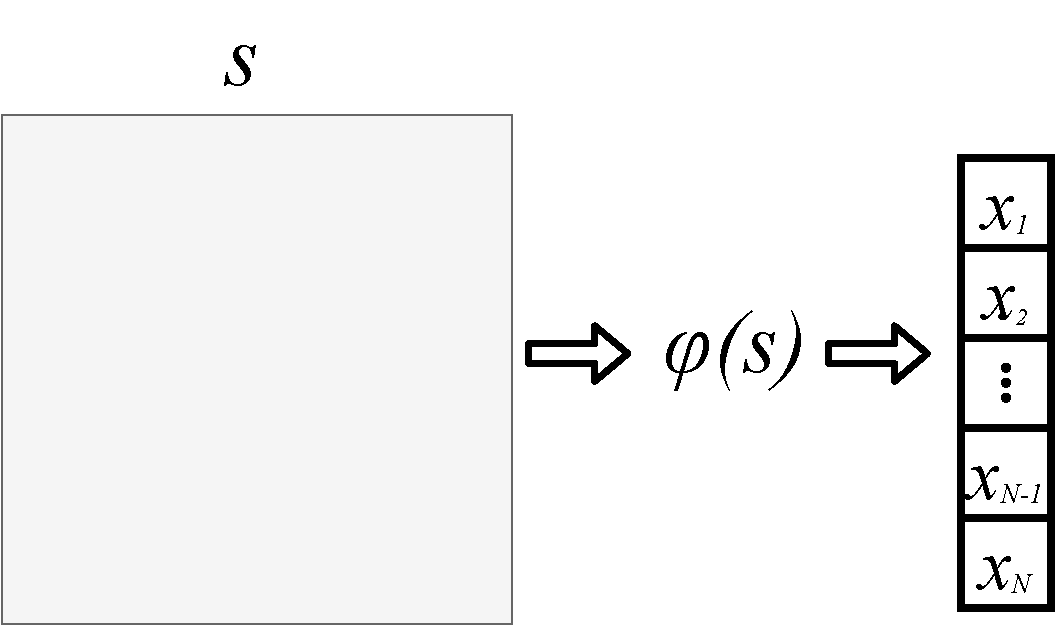
\includegraphics[scale=0.25]{Chapter4/Figs/stox.pdf}
    \caption{La observación $s$ del agente se traduce mediante la función $\phi$ en un vector de variables de alto nivel.}
    \label{fig:obs-to-macro}
\end{figure}

Una vez que se
realiza el mapeo entre el espacio de
estados y el de macro variables, se obtiene una lista  $E$ de variables de interés, las cuales se consultarán en el grafo causal.
Por simplicidad, la lista $E$ se obtiene a través de una función $f$ que calcula cuáles variables tienen un valor diferente entre el vector meta $\mathbf{g}$
y el vector de macro variables $\mathbf{x}$. Se puede suponer que $\mathbf{x} \neq \mathbf{g}$, sin embargo, dado que los ambientes son dinámicos, no se puede asegurar que la configuración inicial de un ambiente no sea igual a la que se desea llegar. 

% A menudo, la meta final de una tarea en RL está compuesta de submetas. Por ejemplo, un brazo robótico cuya meta es mover un objeto de un punto $P_x$ a otro $P_y$, antes debe tomarlo  algunos casos,   
En algunos casos, las variables de interés pueden seguir un orden causal, lo que se puede interpretar como que una meta depende de que se cumplan otras submetas.
Por lo tanto, la lista $E$ puede guardarse en un estructura de datos tal que sus elementos estén ordenados por una función de prioridad, por ejemplo, de acuerdo con el orden topológico de $\mathcal{D}$. Con esto, los elementos con mayor prioridad pueden ser las variables que llevan a cumplir submetas necesarias para alcanzar la meta final.
En la Figura \ref{fig:e-list} se describe un ejemplo de cómo se produce la lista $E$ con respecto al grafo de la Figura \ref{fig:example-d}. 


\begin{figure}[h]
    \centering
    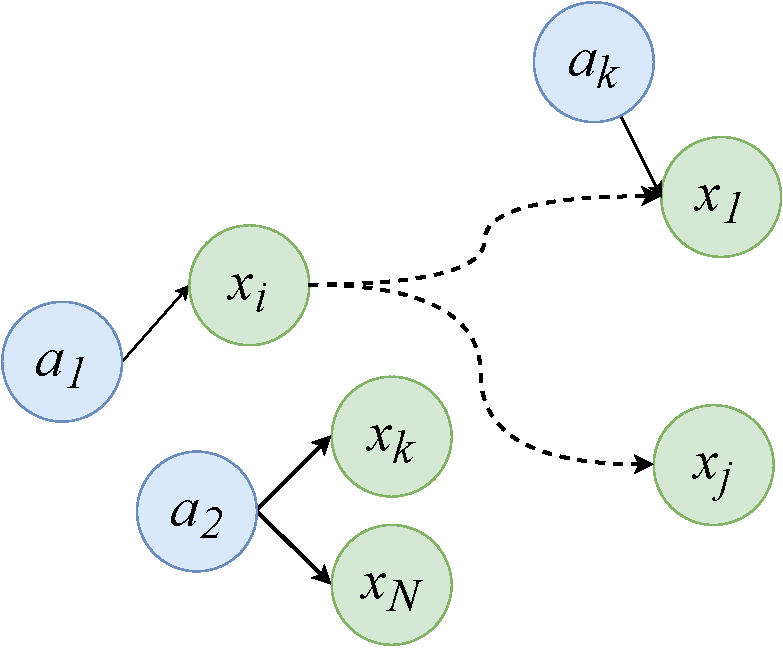
\includegraphics[scale=0.3]{Chapter4/Figs/examplegraph.pdf}
    \caption{Ejemplo de un grafo causal $\mathcal{D}$. Las flechas con cuerpo curvo y punteado denotan caminos causales (notación arbitraria del autor).}
    \label{fig:example-d}
\end{figure} 


\begin{figure}[h]
    \centering
    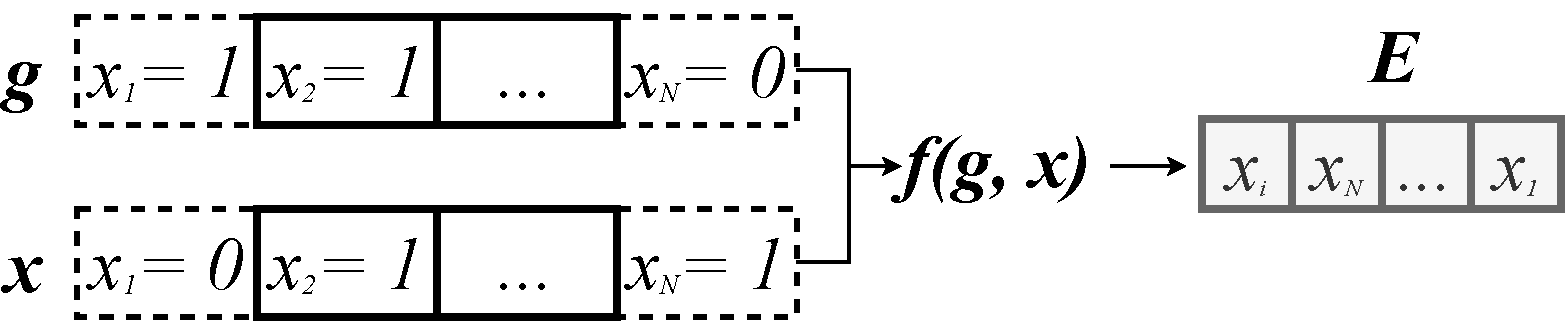
\includegraphics[scale=0.45]{Chapter4/Figs/listofinterest.pdf}
    \caption{La lista $E$ se obtiene de las variables que tienen valores diferentes entre los vectores $\mathbf{x}$ y $\mathbf{g}$. En este ejemplo, se almacenan la variable $x_i$ en $E$ si $|x_i - x_i' | = 1$ tal que $x_i\in \mathbf{g}$ y $x_i' \in \mathbf{x}$. El orden de $E$ sigue el orden topológico de grafo de la Figura \ref{fig:example-d}.}
    \label{fig:e-list}
\end{figure} 

El siguiente paso corresponde a obtener una acción $a \in \mathcal{A}$ para que el agente la lleve a cabo.
Para esto, se hace un recorrido sobre la lista $E$, donde
por cada elemento $e \in E$ se hace una consulta al grafo causal. La consulta consiste en la
obtención de los padres de $e$.  Si $e$ se encuentra en el grafo y además tiene al menos una variable de acción $a$ como predecesor se realiza tal acción.
En este trabajo, solo se abordan problemas donde los grafos causales los vértices que representan las acciones no tienen padres y además no es necesario llevar a cabo varias acciones al mismo tiempo para afectar a $e$.
% Algunos posibles casos de los tipos de conexiones entre las acciones y las variables de interés se pueden ver en la Figura \ref{fig:connection-types}. 
% Las conexiones (a) representan el caso donde una variable de estado $e'$ afecta la acción que se desea tomar.
% % El grafo (b) denota el caso donde para llevar a cabo una acción $a$ es necesario realizar antes la acción $a'$. La estructura (c) muestra el caso donde $e$ solo es afectado cuando varias acciones son ejecutadas al mismo tiempo (el autor añade arbitrariamente una conexión entre las aristas para diferenciar este caso del (d)). 
% Finalmente, el caso atacado en este trabajo es (d), donde la acciones son nodos sin padres y además no es necesario llevar a cabo varias acciones al mimo tiempo para cambiar $e$.

% Esta tesis se limita a trabajar en tareas donde las estructuras causales subyacentes solo contienen conexiones del tipo (d) de la Figura \ref{fig:connection-types}.  

% \begin{figure}
%     \centering
%     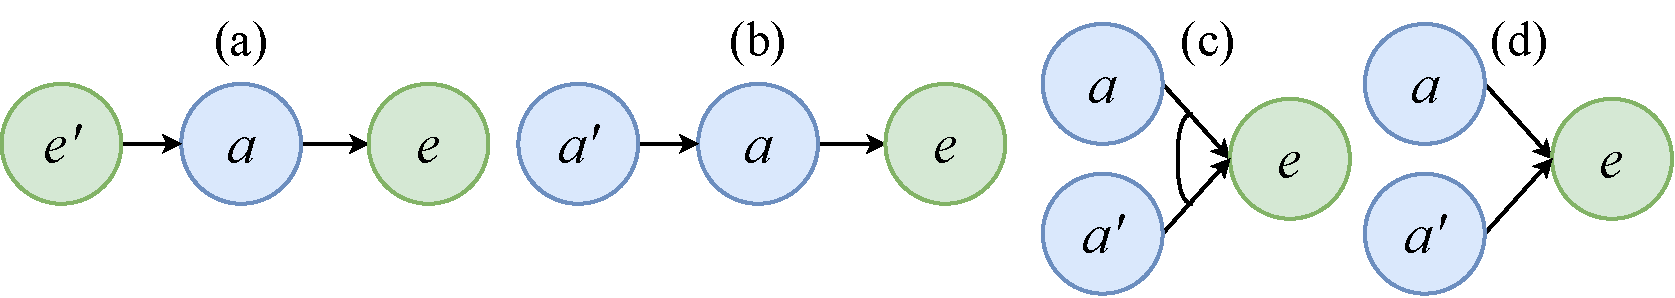
\includegraphics[scale=0.3]{Chapter4/Figs/connections.pdf}
%     \caption{Algunos casos de las conexiones entre la acción $a \in \mathcal{A}$ y la variable de interés $e \in E$. Esta tesis se enfoca en problemas que contienen solo el  caso más simple (d), donde la acción $a$ no depende de que sucedan otras variables $e'$ ni de otras acciones $a'$ (caso (a) y (b), respectivamente). Además, en este tipo de estructuras, no es necesario llevar a cabo más de una acción al mismo tiempo para cambiar el estado de $e$ (caso (c)).}
%     \label{fig:connection-types}
% \end{figure}

% Explicar un poco más esto, como están conectadas estas variables siempre a-x o puede haber algo como a-y-x y el caso de que las causas son independientes entre ellas, tal vez añadir eso en las suposiciones. Como que la x es hija de varias que pasa, tal vez enumerar lo casos
% Caso 1) es una causa directa y no es de efecto común
% caso 2) causa directa y es de efecto común
% caso 3 causa lejana pero no hay más info entonces la ejecuto
% caso 4) o los caoss deben dividirse si son de efecto común o causa común. Este último es complicado porque hacer algo que afecta a otros elementos que no quiero afectar es un problema. Recalcar que casos atacamos
% se regresa una acción aleatoria que es causa directa de esa variable $x_i$. 

% Poner ejemplo, imágenes de los casos? Tal vez solo decir cuál de todas las acciones se selecciona. Enfatizar en que las acciones son independientes. Tal vez una imagen de los posibles casos y además del que se ataca en los dominios propuestos.

% En caso de que no haya información suficiente, es decir, no se encontró ninguna acción realizable, la política regresa una acción aleatoria, por lo que el agente realiza un exploración a ciegas. Para evitar que repetir intentar actuar sobre las variables de interés, aunque tal vez esto no es necesario porque se supone que una vez ya intenté tal acción.
% se obtienen las variables de interés y el orden en que se obtienen las causas de 
% cada variable de interés, se hace un barajado sobre éstas.
% Tal vez todo esto está de más, yo creo que sí por eso de que $E$ está en orden aleatorio ya me quito de todo esto

El método propuesto encaja sin problemas y se incorpora en el algoritmo Q-learning \cite{watkins1992q}. El proceso de entrenamiento 
 del algoritmo Q-learning se mantiene idéntico salvo por  la selección de acciones guiada.
En los Algoritmos
\ref{alg:q-algo-extra-info} y \ref{alg:dqn-algo-causal}, se presentan los métodos resultantes al añadir la selección de acciones guiada, Q-learning clásico y DQN, respectivamente. Además, se puede notar que el proceso de selección de acción propuesto no está atado a un esquema $\epsilon$-greedy. Se podría utilizar otro método basado en política, por ejemplo, donde antes de utilizar la política que se está aprendiendo, se consulte el modelo causal. Sin embargo, explorar otros esquemas de selección queda fuera de este trabajo.

\begin{mialgoritmo}[H]
  	\caption{$Q$-learning guiado por conocimiento causal}
	\label{alg:q-algo-extra-info}
  \begin{algorithmic}[1]
  \setstretch{1}
  \REQUIRE Estructura causal $\mathcal{D}$, la meta $\mathbf{g} = [x_1, \dots, x_N]$ donde $x_i \in \mathcal{X}$, la tasa de aprendizaje $\alpha \in (0,1]$, el número de episodios $k$, el horizonte $H$ de cada episodio, el coeficiente $\delta$, los valores $\epsilon_{\max}$ y $\epsilon_{\min}$.
  \STATE Inicializar arbitrariamente $Q(s,a)$, para todo $s\in \mathcal{S}$ excepto donde $Q(terminal, \cdot) = 0$.
  
  \FOR{$episodio = 1, \dots, k$}
    \STATE Inicializar $s_0$.
    \FOR{$t = 0, \dots, H$}
    \STATE $\epsilon \leftarrow \max(\epsilon_{\min}, \epsilon_{\max} - \frac{|\epsilon_{\max} - \epsilon_{\min}| \times t}{H \times k \times \delta})$.
    \STATE Elegir $a_t$ usando el Algoritmo \ref{alg:guided-action-selection}, que recibe como entrada $\mathcal{D}$, $\mathbf{g}$, $s_t$ y $\epsilon$.
    \STATE Tomar acción $a_t$ y observar $r_{t+1}, s_{t+1}$.
    \STATE $Q(s_t, a_t) \leftarrow Q(s_t, a_t) + \alpha [r_{t+1} + \gamma \max_a Q(s_{t+1}, a) - Q(s_t, a_t)]$.
    \STATE $s_t \leftarrow s_{t+1}$.
    \ENDFOR
  \ENDFOR
  \end{algorithmic}
\end{mialgoritmo}


\begin{mialgoritmo}[H]
  	\caption{DQN guiado por conocimiento causal.}
	\label{alg:dqn-algo-causal}
  \begin{algorithmic}[1]
  \setstretch{1}
  \REQUIRE Estructura causal $\mathcal{D}$, la meta $\mathbf{g} = [x_1, \dots, x_N]$ donde $x_i \in \mathcal{X}$, el número de episodios $k$, el horizonte $H$ de cada episodio, el coeficiente $\delta$, los valores $\epsilon_{\max}$ y $\epsilon_{\min}$.
  \STATE Inicializar búfer de experiencias $D$ con capacidad $M$, la función de valor de acción $Q$ con pesos aleatorios $\theta$ y la función de valor de acción objetivo $\hat{Q}$ con pesos $\theta^- = \theta$.
  
  \FOR{$episodio = 1, \dots, k$}
    \STATE Inicializar $s_0$.
    \FOR{$t = 0, \dots, H$}
    \STATE $\epsilon \leftarrow \max(\epsilon_{\min}, \epsilon_{\max} - \frac{|\epsilon_{\max} - \epsilon_{\min}| \times t}{H \times k \times \delta})$.
    \STATE Elegir $a_t$ usando el Algoritmo \ref{alg:guided-action-selection}, que recibe como entrada $\mathcal{D}$, $\mathbf{g}$, $s_t$ y $\epsilon$.
    \STATE Tomar acción $a_t$, observar recompensa $r_{t}$ e imagen $s_{t+1}$.
    % \STATE Asignar $s_{t+1} =  s_t, a_t, x_{t+1}$ y preprocesar $\phi_{t+1} = \phi(s_{t+1})$.
    \STATE Guardar transición $(s_t, a_t, r_t, s_{t+1})$ en $D$.
    \STATE De $D$ tomar una muestra aleatoria de un lote de transiciones $(s_j, a_j, r_j, s_{j+1})$.
    \STATE Establecer
	\[
	 y_j = 
   \begin{cases} 
      r_j  & \mbox{si el episodio termina en el paso } j + 1 \\
      r_j + \gamma \max_{a'}\hat{Q}(s_{j+1}, a'; \theta^-) & \mbox{en cualquier otro caso.}
   \end{cases}
	\]
	\STATE Realizar el paso del
	descenso de gradiente sobre $(y_j -  Q(s_j,a_j;\theta))^2$ con respecto a los parámetros de la red $\theta$.
	\STATE Cada $C$ pasos reiniciar $\hat{Q} = Q$.
    \ENDFOR
  \ENDFOR
  \end{algorithmic}
\end{mialgoritmo}


\section{Ejemplo: Problema de los interruptores de luz}\label{section:switches-example}

En esta sección se describe un ejemplo sobre un problema en que se realizan 
lo experimentos de esta investigación. Por ahora, solo se describe el problema
y cómo se aplica el método propuesto.

Imagina que construyes un robot llamado Joi, con el propósito de prender o apagar las luces de las habitaciones 
de una casa de acuerdo a como se le comande.
A Joi se le puede dotar de cierto conocimiento previo de la configuración
del cableado de la casa, tal que le ayude a descifrar las correspondencias entre
interruptores de luz y los focos de las habitaciones. 
 A Joi le gusta aprender mediante prueba
 y error y recibir una señal de recompensa positiva o negativa de acuerdo a su comportamiento. Además, el robot 
 necesita repetir muchas veces la misma acción para aprender
 qué provocará realizarla. Por lo tanto, si Joi conoce los efectos de algunas de sus acciones (mover los interruptores), puede reducir sus intentos para
 resolver las conexiones entre interruptores y los focos. 
 Por ejemplo, con anticipación Joi puede saber que el mover interruptor de luz $i$ causa que
prenda o apague la luz de la cocina.
 Así que al darle la orden de prender las luces de la cocina, el baño y de alguna otra habitación, Joi solo se enfoca en aprender las partes que no
 conoce.
 
 El problema se puede ver como una tarea donde es necesario tomar las
 decisiones adecuadas para llegar a un configuración de luces deseada. Formalmente, se puede ver como un MDP condicionado a metas donde 
 
 \begin{itemize}
     \item El espacio de estados $\mathcal{S}$, es el conjunto de
     posibles observaciones de la casa desde una vista cenital como en la Figura
   \ref{fig:obs-switches}.
     \begin{figure}[H]
         \centering
         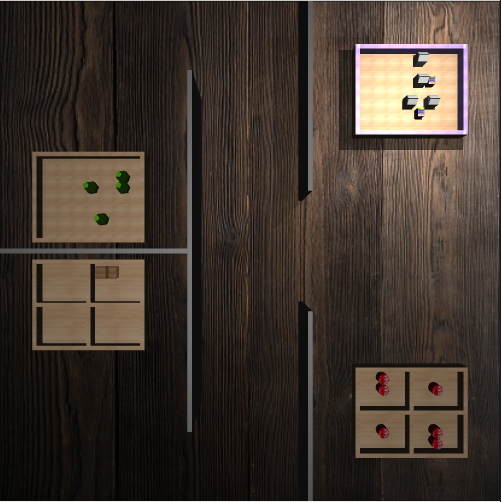
\includegraphics[scale=0.17]{Chapter4/Figs/example_obs.png}
         \caption{Observación disponible para el robot.}
         \label{fig:obs-switches}
     \end{figure}
     \item El espacio de acciones es $\mathcal{A} = \{a_1, a_2, \dots, a_N\}$
     donde cada $a_i$ corresponde a mover o no el interruptor de luz $i$. $a_i = 0$ si no se mueve el interruptor y $a_i = 1$ si se mueve.
     \item El conjunto de variables de alto nivel $\mathcal{X} = \{x_1, x_2, \dots, x_N\}$ contiene
     a las variables que describen el estado de cada foco en la casa. Por ejemplo, $x_i = 1$ establece que el foco $i$ está prendido.
     \item El grafo causal $\mathcal{D} = <\mathcal{A'}, \mathcal{X'}>$, donde
     $\mathcal{A'} \subseteq \mathcal{A}$ y $\mathcal{X'} \subseteq \mathcal{X}$, visualmente el grafo se puede representar como en la Figura \ref{fig:dag-example-switches}.
     
     \begin{figure}[H]
         \centering
         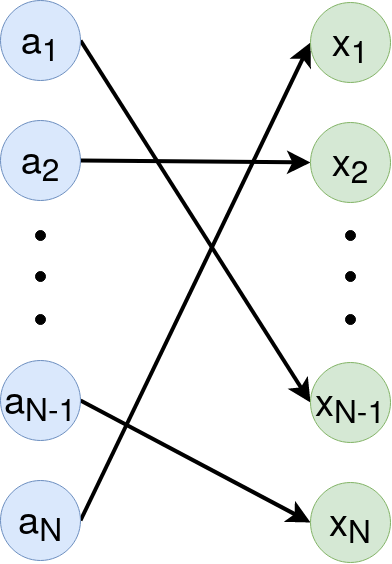
\includegraphics[scale=0.2]{Chapter4/Figs/graph.png}
        \caption{Una estructura causal posible para $N$ interruptores y $N$ luces
        con un tipo de conexión uno-a-uno.}
        \label{fig:dag-example-switches}
     \end{figure}
     \item No se cuenta con la función de transición $\mathcal{P}$, sin embargo,
     se conoce que el interruptor $i$ no necesariamente corresponde al foco $i$.
     \item El espacio de metas $\mathcal{G}$ contiene a todas las
     combinaciones posibles de focos prendidos y apagados en la casa.
     \item La recompensa inmediata $r$ se calcula a través de medir la diferencia entre la observación y la meta.
 \end{itemize}
 
 Una vez que la tarea se ha descrito como un MDP, es posible que Joi
 aprenda a alcanzar una configuración de luces deseada
 utilizando un algoritmo de RL, Q-learning por ejemplo. Además,
 dado que suponemos que Joi puede aprovechar el conocimiento que le
 ofrece el grafo causal $\mathcal{D}$, la selección de acciones se puede
 guiar usando el Algoritmo \ref{alg:guided-action-selection}. 
 En la Figura \ref{fig:example-switches} se muestra un paso en el proceso de aprendizaje.
 
 \begin{figure}
     \centering
     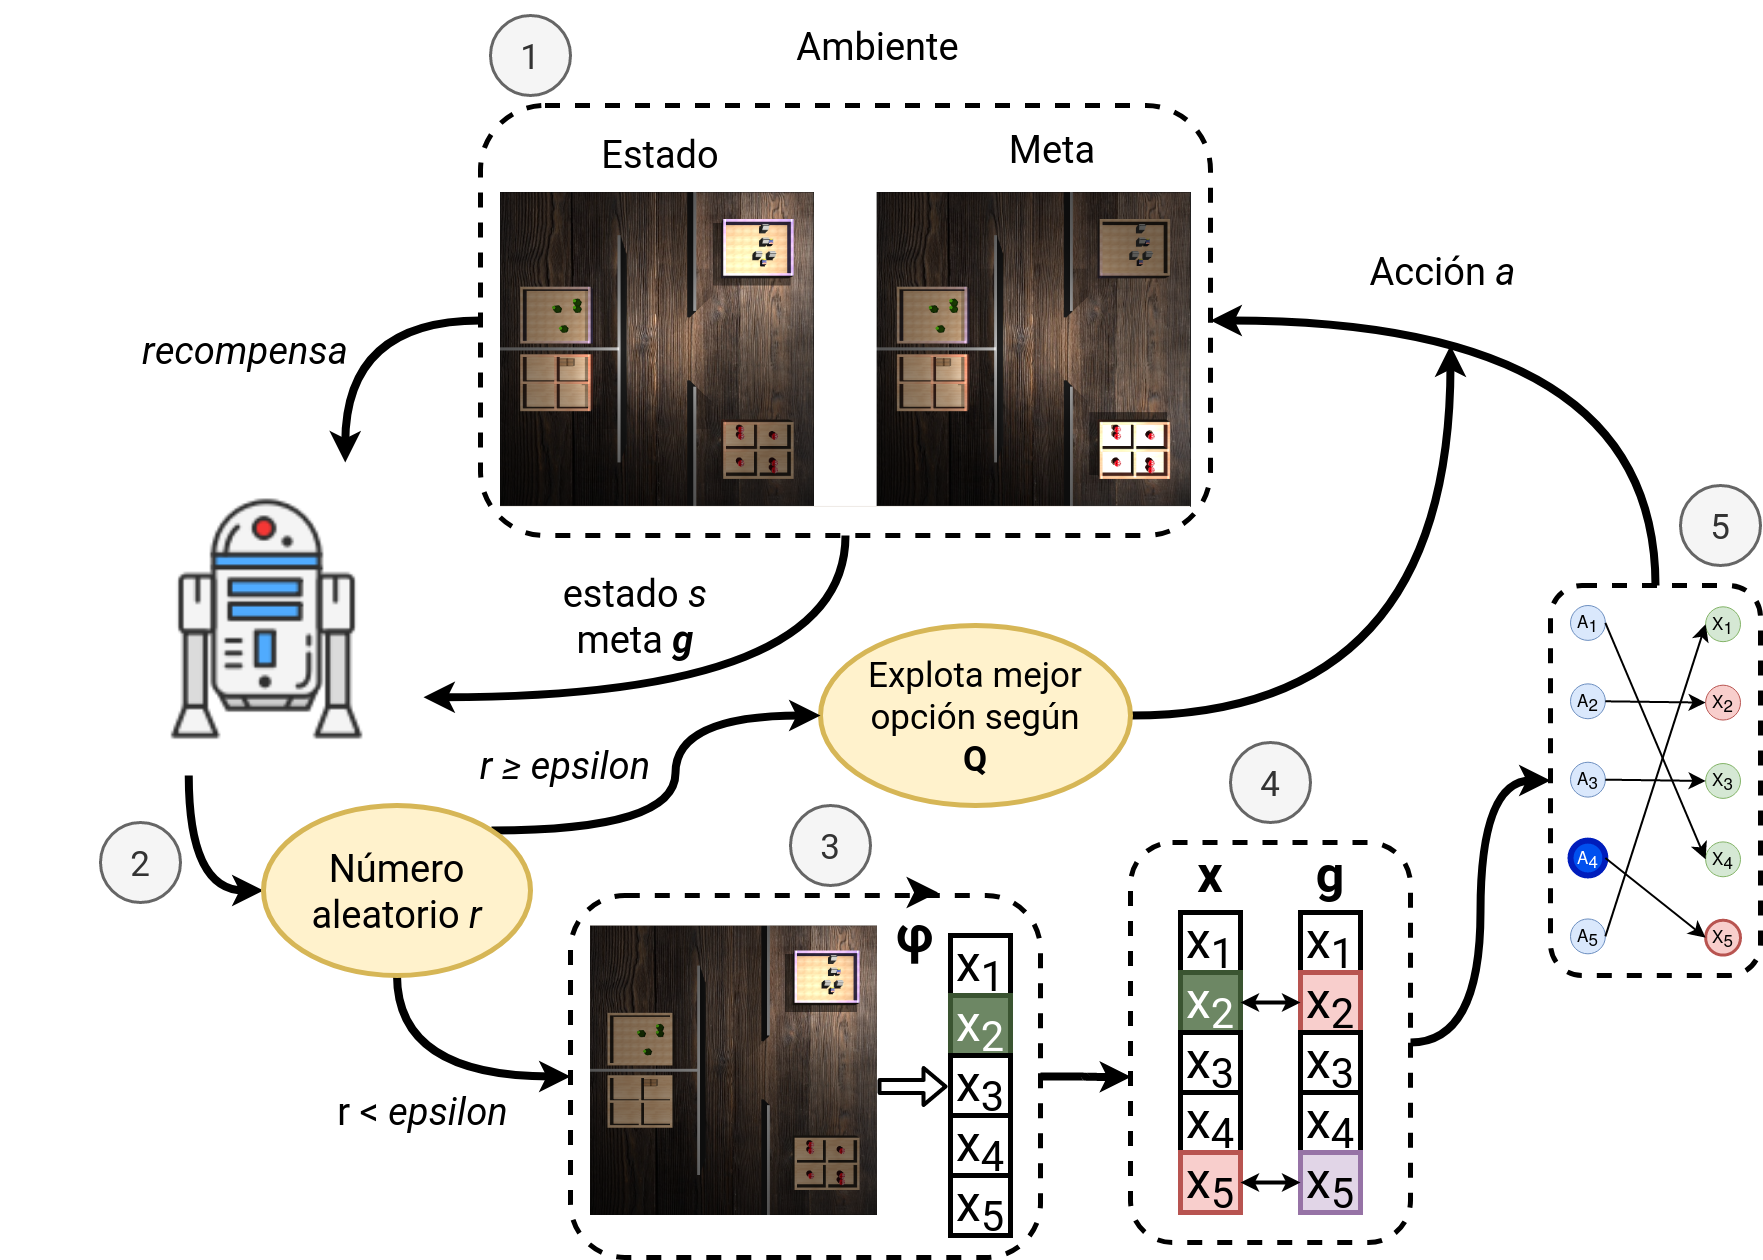
\includegraphics[scale=0.25]{Chapter4/Figs/example_method.png}
     \caption{Interacción del agente con su ambiente: 1) el agente observa el estado de su ambiente además de conocer el vector $\mathbf{g}$, 2) inicia
     la política de selección de acciones, 3) si el agente debe explorar, mapea la observación a un vector de variables de alto nivel $\mathbf{x}$, 4) se calculan los diferentes entre los vectores $\mathbf{x}$ y $\mathbf{g}$, 5) se consultan los padres de las variables de interés y se retorna la acción. El entrenamiento continúa su aprendizaje de manera normal.}
     \label{fig:example-switches}
 \end{figure}
 
 \clearpage
 \section{Resumen}
 
En este capítulo se presentó el tipo de tareas que se 
desean atacar junto con el método propuesto. La propuesta
integra un modelo causal en un algoritmo de aprendizaje por refuerzo para
acelerar su aprendizaje.
Las tareas que se desean atacar, son 
planteadas como procesos de decisión de Markov dirigidos por metas.
La principal característica de este tipo de problemas, que es de interés para este trabajo,
es el contar con una estructura causal del ambiente en un espacio 
que puede ser de menor dimensión que el de las observaciones.
El método propuesto se puede dividir en dos partes, que
corresponden con las contribuciones de este trabajo:

\begin{enumerate}
    \item \textit{Una representación de las relaciones causales del mundo del agente.} Para hacer consultas sobre un modelo causal del ambiente, se utiliza la estructura causal $\mathcal{D}$, la cual tiene como vértices las variables de estado y de acción.
    \item  \textit{Un esquema de interacción entre un algoritmo de aprendizaje por refuerzo
    y un modelo causal}. Se introduce un algoritmo basado en la política de selección
    de acciones $\epsilon$-greedy, el cual guía la elección de acciones de acuerdo a la estructura $\mathcal{D}$, del modelo causal.
\end{enumerate}

\chapter{Experimentos y resultados}\label{chapter5}

% **************************** Define Graphics Path **************************
\graphicspath{{Chapter5/Figs/}}


En este capítulo se describe la experimentación y lo resultados obtenidos
que muestran la mejora en el desempeño de un agente que aprende
con y sin información adicional de un grafo causal.
Para probar el concepto propuesto se atacan dos problemas: la tarea de clásica del taxi \cite{Dietterich:2000:HRL:1622262.1622268} y la de los
interruptores de luz, descrita en el Capítulo \ref{chapter4}.
En resumen, los experimentos consisten en integrar el grafo $\mathcal{D}$ a la política $\epsilon$ greedy
en el algoritmo $Q$-learning \cite{watkins1992q}.
En la política $\epsilon$-greedy en vez de mantener fijo a $\epsilon$, se propone empezar motivando al agente a explorar y usar
el modelo causal e ir disminuyendo $\epsilon$ para dar más peso a la explotación.
Se comparan cuatro algoritmos, \textit{Q-learning sin información
adicional}, \textit{Q-learning con una estructural causal completa}, \textit{Q-learning con una estructura parcial} y un \textit{Q-learning con una estructura incorrecta}.
Cada uno de los algoritmos se ejecuta en una versión determinista y 
otra estocástica del ambiente. 
En las siguientes secciones se describen a detalle los experimentos realizados y los resultados. Todo el software desarrollado está 
disponible en \url{https://github.com/ivanfeliciano/causal_rl/}.


\section{Problema del taxi}

\subsection{Descripción de la tarea}

El primer problema a resolver es la tarea clásica del taxi \cite{Dietterich:2000:HRL:1622262.1622268}.
La Figura \ref{fig:taxi} muestra gráficamente el problema.
Existen cuatro posiciones en el mundo marcadas como R, B, G, y Y. 
La tarea es episódica. En cada episodio, 
el taxi comienza en un cuadro aleatoriamente elegido. 
Existe un pasajero en una de la cuatro posiciones (también elegida
aleatoriamente), y el pasajero desea ser transportado a una de las
cuatro zonas.
El taxi debe dirigirse a la posición del pasajero, recogerlo, ir a su destino y dejarlo.
El episodio termina cuando el pasajero es dejado en su destino.

\begin{figure}[H]
    \centering
    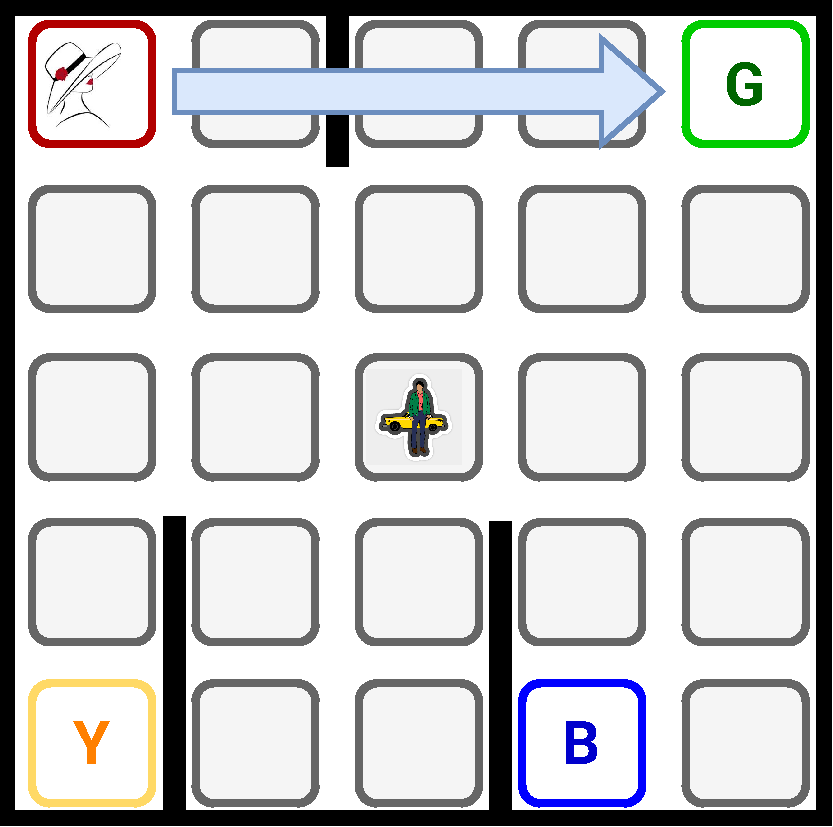
\includegraphics[scale=0.25]{Chapter5/Figs/taxi-env.pdf}
    \caption{La cuadrícula del ambiente del taxi. El taxi se encuentra en el cuadro central. En esta configuración del mundo, el objetivo es recoger al pasajero en la posición R y llevarlo a la posición G.}
    \label{fig:taxi}
\end{figure}

El conjunto de acciones $\mathcal{A}$ está compuesto por seis elementos: una acción para recoger $a_1$, una para dejar $a_2$ y
cuatro acciones de 
navegación que trasladan al taxi un cuadro al norte, sur, 
este u oeste, denotadas por $a_3, \dots, a_6$, respectivamente.
Existe una recompensa de -1 por cada acción, una recompensa adicional de 20 por cada pasajero llevado a su destino 
exitosamente y una penalización de -10 por acciones ilegales
de recolección y dejado.
El espacio de estados $\mathcal{S}$ tiene como elementos 
500 tuplas de tres elementos donde describen los 25 cuadros, las 5 posiciones del pasajero (incluyendo cuando está en el taxi) y los 4 destinos.


% Aquí ahondar más sobre el conjunto X y G, quienes lo compoenen y como está de pequeñito el problema
El conjunto $\mathcal{X}$ contiene 4 variables que traducen las tuplas con las posiciones del taxi y del pasajero en variables binarias. $x_1$
es la variable que dice si el taxi está en la misma posición que el
pasajero, $x_2$ es la variable que denota si el pasajero es llevado dentro del taxi, $x_3$ describe si el taxi está en la posición destino,
y $x_4$ es la variable que representa al estado de que el pasajero es entregado correctamente. Es una tarea relativamente simple y $x_1 \neq x_3$, por lo tanto las metas son $\mathcal{G} = \{\mathbf{g_1}, \mathbf{g_2}\}$, donde $\mathbf{g_1} = [1, 1, 0 , 0]$ y $\mathbf{g_2} = [0,1,1,1]$. El primer vector se puede ver como el sub objetivo de 
llevar subir al pasajero al taxi y el segundo vector es la meta general, 
entregar al pasajero en su destino.
El grafo causal $\mathcal{D}$ entre las variables de acción y los estados se puede 
ver en la Figura \ref{fig:cm-taxi}. Para este problema, los efectos
necesitan de todas sus causas para suceder, por ejemplo, para que el
pasajero esté dentro del taxi, $x_2 = 1$, entonces se debe actuar
subiéndolo al vehículo $a_1$ y además estar en la misma ubicación que
el pasajero.

\begin{figure}[H]
    \centering
    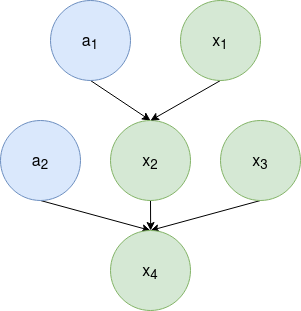
\includegraphics[scale=0.3]{Chapter5/Figs/causal_structure_taxi.png}
    \caption{Propuesta de una estructura causal para la tarea del taxi.}
    \label{fig:cm-taxi}
\end{figure}


\subsection{Configuración experimental}

Debido a la poca información que ofrece el grafo $\mathcal{D}$ y al tamaño de $\mathcal{G}$, para este problema no se ahonda en realizar experimentos con diferentes configuraciones. Por lo
tanto, sólo se comparan dos algoritmos,
el algoritmo Q-learning con y sin la estructura causal.
Además, los dos algoritmos se prueban sobre dos versiones del ambiente, una determinista
y otra estocástica. Los valores de los parámetros para los experimentos se muestran en el Cuadro \ref{tab:tax-params}. Se ejecutan $M$ experimentos y cada experimento consiste de ejecutar cada algoritmo $k$ de episodios. La medida
de desempeño es la recompensa promedio por episodio. El valor de $\epsilon$ se va decrementando en cada paso de tiempo de entrenamiento $t$ de forma lineal ($\epsilon = \max(\epsilon_{\min}, mt + \epsilon_{\max})$, $m < 0$ y representa la tasa de decremento)
con respecto al
número de episodios, por lo que se fomenta la exploración y el uso del modelo causal al principio y posteriormente se explota la información de $Q$.

\begin{table}[H]
\centering
\caption{Parámetros para las versiones del algoritmo Q-learning.}
\label{tab:tax-params}
\begin{tabular}{ll}
\hline
Parámetro                                                                                      & Valor    \\ \hline
$\alpha$                                                                                       & 0.8      \\
$\gamma$                                                                                       & 0.95     \\
$\epsilon_{\min}$                                                                              & 0.1      \\
$\epsilon_{\max}$                                                                              & 1.0      \\
$m$                                                                                            & -0.0045 \\
$k$                                                                                            & 5000     \\
$M$                                                                                            & 10       \\
\begin{tabular}[c]{@{}l@{}}Probabilidad de\\ transición en ambiente\\ estocástico\end{tabular} & 0.7      \\ \hline
\end{tabular}
\end{table}

\subsection{Resultados}

En la Figura \ref{fig:results-taxi} se muestran los resultados obtenidos
para ambas configuraciones del ambiente (determinista y estocástico) donde
los valores de los parámetros se describen en el Cuadro \ref{tab:tax-params}.
La recompensa promedio por episodio para el método propuesto y para el algoritmo
original Q-learning están en color naranja y azul, respectivamente. 
Los resultados muestran que el algoritmo Q-learning guiado por el grafo da un salto inicial alto y mantiene una recompensa promedio mucho mayor que la versión sin información adicional. Esto era esperado, ya que 
no inicia una exploración a ciegas. Por otra parte, para el caso 
del ambiente estocástico, parecen comportarse de manera similar después de los
primeros 1000 episodios. Esto se puede deber a que tal vez la información del 
grafo no ayuda los suficiente, ya que a pesar de que tal vez existen
conexiones entre acciones y estados que no se están tomando en cuenta.


\begin{figure}[H]
  \centering
  \subfloat[Ambiente determinista.]{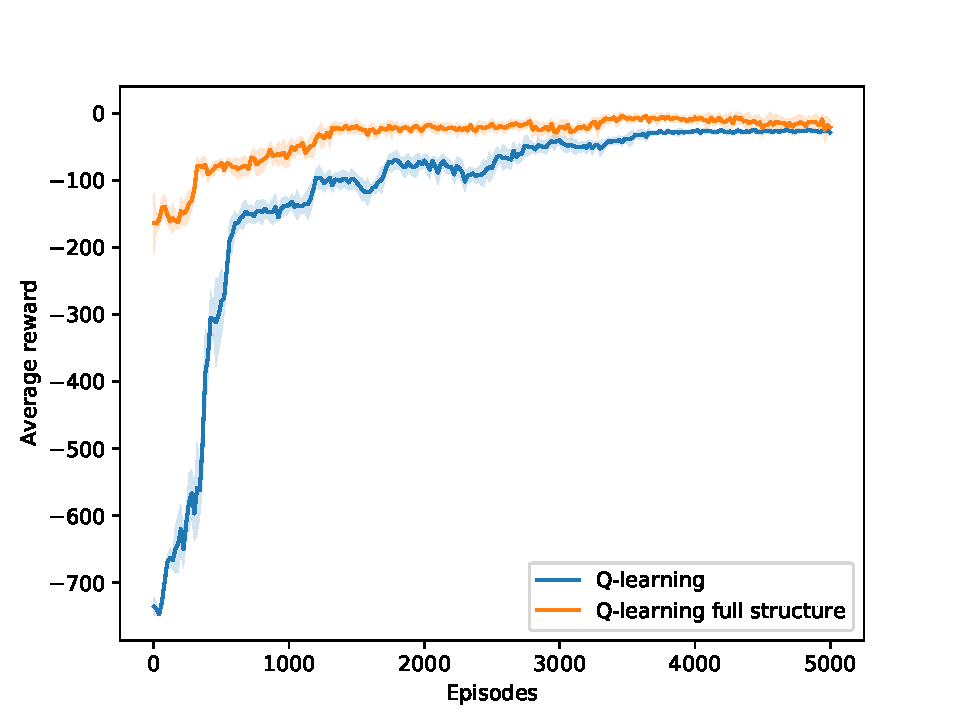
\includegraphics[width=0.5\textwidth]{Chapter5/Figs/taxiDet500010.pdf}\label{fig:taxi-rew-det}}
  \hfill
  \subfloat[Ambiente estocástico.]{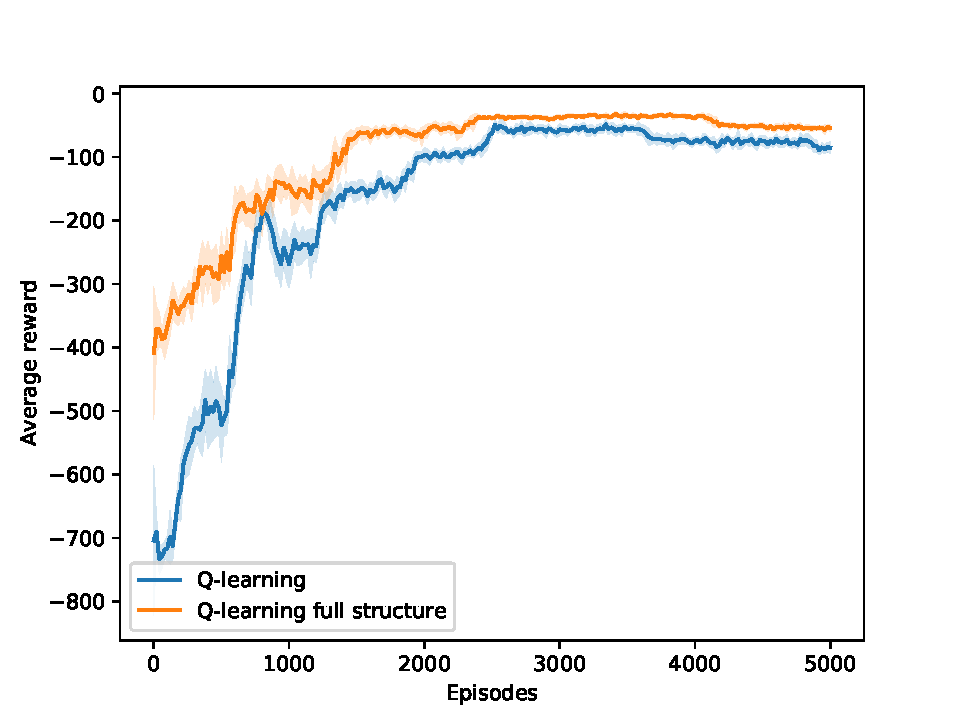
\includegraphics[width=0.5\textwidth]{Chapter5/Figs/taxiSto500010.pdf}\label{fig:taxi-rew-sto}}
  \caption{Comparación del desempeño para los dos algoritmos en 5000 episodios. La región sombreada es la desviación estándar para 10 experimentos.}
  \label{fig:results-taxi}
\end{figure}
\section{Problema de los interruptores de luz}

\subsection{Descripción de la tarea}
Para los experimentos de esta sección se ataca la tarea de control de interruptores de luz propuesta en \cite{nair2019causal} y descrita de manera general en la Sección \ref{section:switches-example}. Un agente tiene el control
de $N$ interruptores que controlan $N$ luces en un sitio.
Cada acción $a\in \mathcal{A}$ corresponde a mover un interruptor o 
a no mover ninguno, por lo tanto $|\mathcal{A}| = N + 1$.
El agente puede percibir dos tipos de señales del ambiente,
una imagen $s$ con una vista cenital del sitio, o vectores binarios $x \in \{0,1\}^N$ de 
macro-variables que codifican las luces prendidas, donde
$x_i = 1$ si la luz en la zona $i$ está prendida, de otro modo 
toma el valor $x_i = 0$.

Se exploran tres tipos de estructuras causales entre los
interruptores y las luces: \textit{uno-a-uno},
\textit{causa común} y \textit{efecto común}.
En los problemas con estructuras uno-a-uno cada interruptor corresponde a una sola luz.
Para el segundo tipo, de causa común, todas
las luces son controladas a lo más por un interruptor pero un
solo interruptor puede controlar más de una luz.
El tercer caso son estructuras de efecto común, donde cada interruptor
controla una sola luz, aunque múltiples interruptores
pueden controlar la misma luz. De manera visual, los tres tipos de estructuras
se muestran en la Figura \ref{fig:struct}.

\begin{figure}[H]
    \centering
    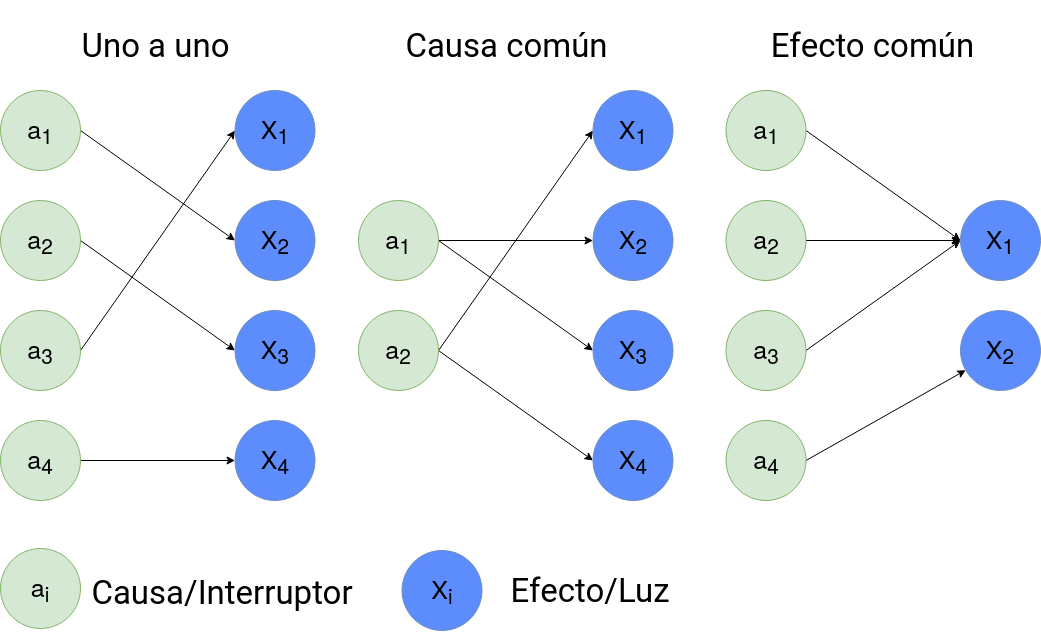
\includegraphics[scale=0.3]{Chapter5/Figs/switches_struct.png}
    \caption{Tipos de estructuras causales subyacentes posibles.}
    \label{fig:struct}
\end{figure}
La recompensa inmediata $r$ brindada al agente se calcula obteniendo la distancia entre el vector de variables de estado alto nivel $\mathbf{x}$ y el vector meta $\mathbf{g}$. En este problema se usa la distancia euclidiana.


\subsection{Configuración experimental general}

En las siguientes secciones se compara el desempeño 
del método propuesto en diferentes escenarios, principalmente, para mostrar 
las posibilidades y ventajas de usar un información del grafo causal, completa, incompleta e incluso incorrecta. 
% A pesar de ser diferentes
% experimentos, éstos comparten la configuración de algunos elementos, por ejemplo, 
% la medida de desempeño, el número de variables $N$, etc.
Se comparan cuatro algoritmos, teniendo como base
el método Q-learning. Donde la diferencia subyace en la cantidad y calidad de la información adicional con la que cuenta. A continuación, se describen de manera breve los métodos
comparados.

\begin{itemize}
    \item \textit{Q-learning sin información adicional}. Este método sirve como
    línea de base para medir que tanto mejora el aprendizaje. El algoritmo, dependiendo del espacio de estados sobre el que se trabaje, es el 
    método básico de Q-learning \cite{watkins1992q} o Q-learning profundo \cite{mnih2013playing}, para estados
    discretos y continuos, respectivamente. La selección de acciones se lleva a cabo mediante una política $\epsilon$ greedy clásica.
    \item \textit{Q-learning + estructura causal completa}. Durante la política de selección de acciones, el agente cuenta con la estructura causal del ambiente completa y verdadera $\mathcal{D}$.
    \item \textit{Q-learning + estructura causal incompleta}. En este caso, el agente cuenta con un subgrafo $\mathcal{D'}$ del grafo $\mathcal{D}$. Este subgrafo se genera eliminando aristas de $\mathcal{D}$ aleatoriamente.
    \item \textit{Q-learning + estructura causal incorrecta}. Este algoritmo consulta un modelo $\mathcal{D}''$ con relaciones espurias y sin algunas relaciones verdaderas. Este grafo $\mathcal{D}''$ se obtiene generando un subgrafo de $\mathcal{D}$ como en el caso anterior y agregando aristas aleatoriamente.
\end{itemize}

\begin{figure}
  \centering
  \subfloat[$\mathcal{D}$.]{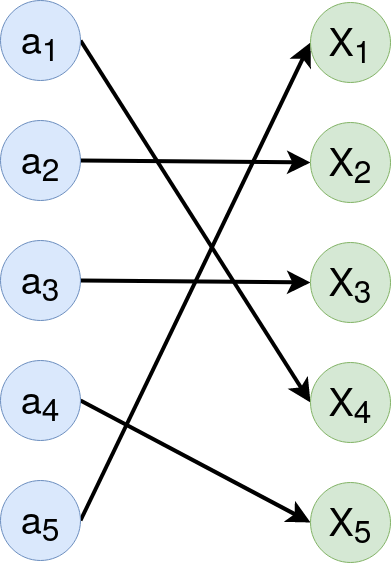
\includegraphics[width=0.2\textwidth]{Chapter5/Figs/completeD.png}\label{fig:completeD}}
  \qquad
  \subfloat[$\mathcal{D}'$]{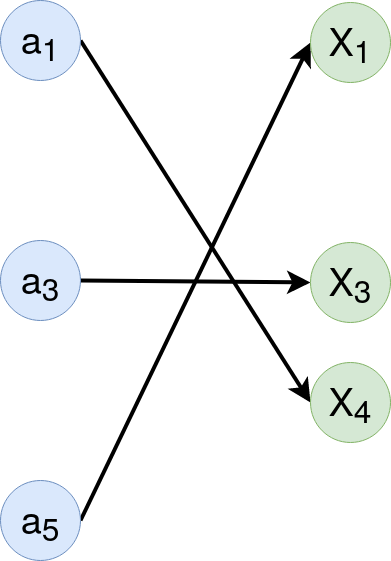
\includegraphics[width=0.2\textwidth]{Chapter5/Figs/incompleteD.png}\label{fig:incompleteD}}
%   \hfill
    \qquad
  \subfloat[$\mathcal{D}''$]{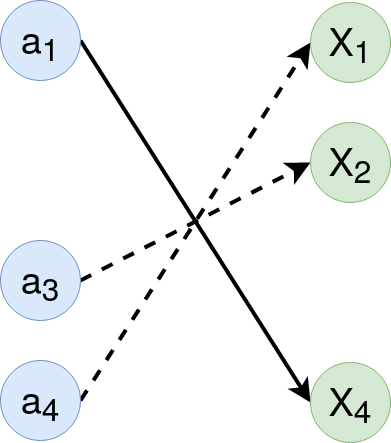
\includegraphics[width=0.2\textwidth]{Chapter5/Figs/wrongD.png}\label{fig:wrongD}}
  \caption{Ejemplo de los tres tipos de información con los que puede  contar el algoritmo Q-learning. El tipo de estructura
  del problema es uno-a-uno. Las aristas dirigidas punteadas describen conexiones espurias.}
  \label{fig:types-info-dag}
\end{figure}

Para medir el desempeño de los algoritmos se evalúa la recompensa
promedio sobre una serie de experimentos.
Cada experimento consiste en ejecutar el algoritmo de aprendizaje durante $k$ episodios, en 
un ambiente con una estructura causal fija $\mathcal{D}$ y donde se busca alcanzar la meta $\mathbf{g}$.
La recompensa promedio para el $i$ ésimo episodio está dada por
$R^{i} = \frac{1}{H}\sum_{t=0}^H r(\mathbf{x}_t, \mathbf{g})$,
donde $H$ corresponde al tamaño del episodio.
El vector $\mathbf{R_i}$, del $i$ ésimo experimento contiene las recompensas promedio por cada episodio, y se define como
$\mathbf{R_i} = (R^{1}, \dots, R^k)$.

Finalmente, la medida de comparación entre algoritmos es
el promedio de los vectores $\mathbf{R_i}$, $i\in [1, M]$,  obtenidos en $M$ experimentos. Esta medida, denotada como  $average$ puede escribirse como 
\begin{equation}
\label{eq:average}
average(\mathbf{R_1}, \dots, \mathbf{R_M}) = \frac{1}{M}(\sum^M_i \mathbf{R_{i}^1}, \dots, \sum^M_i\mathbf{R_{i}^k}),    
\end{equation}

donde $M$ es el número de experimentos y el $\mathbf{R_i^j}$ indica la recompensa promedio obtenida en el $j$ ésimo episodio del $i$ ésimo experimento.

El parámetro $\epsilon$ se disminuye linealmente, donde
en cada selección de acción va decreciendo hasta llegar
un valor mínimo. La regla de actualización de $\epsilon$ en
el paso de tiempo $t$ se puede definir como $\epsilon = \max(\epsilon_{\min}, (\epsilon_{\min} - \epsilon_{\max}) \times t/ (N \times k \times \delta) + \epsilon_{\max})$. Donde $0 < \delta \leq 1$, es un factor para controlar
que tan rápido se alcanza el valor de $\epsilon$  mínimo, entre más cercano a 0,
termina más rápido la exploración.
% Con excepción
% del Experimento 2 (Sección \ref{subsection:exp-epsilon}), donde se cambia el denominador de la
% tasa de decremento para que éste se más rápido.

%Los experimentos se llevan a cabo en dos versiones del ambiente, una discreta y otra estocástica. 
Son tres los experimentos que se realizan. El primer experimento tiene 
como objetivo mostrar el comportamiento de modificar a
diferentes porcentajes la estructura causal $\mathcal{D}$ para obtener $\mathcal{D'}$ y $\mathcal{D}''$. El segundo experimento es con respecto a cambiar la tasa de decremento
de $\epsilon$ para llegar más rápido o lento a explotar 
más constantemente. El tercer experimento, es probar
el algoritmo cuando no se tienen las variables
de alto nivel como observaciones directas, por lo tanto,
se trabaja sobre un espacio de estados continuo. En general,
algunos de los parámetros que se comparten entre los experimentos se muestran en el Cuadro \ref{tab:switch-params}.

\begin{table}[H]
\centering
\caption{Valores para algunos parámetros de los algoritmos.}
\label{tab:switch-params}
\begin{tabular}{ll}
\hline
Parámetro                                                                                      & Valor    \\ \hline
$\alpha$                                                                                       & 0.8      \\
$\gamma$                                                                                       & 0.95     \\
$\epsilon_{\min}$                                                                              & 0.1      \\
$\epsilon_{\max}$                                                                              & 1.0      \\
$N$                                                                                            & \{5, 7, 9\} \\
$H$                                                                                            & \{5, 7, 9\} \\
$k$                                                                                            & \{200, 10000, 200000\}\\
$M$                                                                                            & 10       \\
\begin{tabular}[c]{@{}l@{}}Probabilidad de\\ transición en ambientes\\ estocástico\end{tabular} & 0.75      \\ \hline
\end{tabular}
\end{table}

\newpage
\subsection{Variando el porcentaje de modificación del grafo causal}

\subsubsection{Configuración experimental}

\begin{itemize}
    \item El espacio de estados es discreto, es decir, el agente puede
    obtener las variables $\mathcal{X}$ directamente del ambiente.
    \item Se prueba modificando el grafo $\mathcal{D}$ para obtener a los
    grafos $\mathcal{D'}$ y $\mathcal{D''}$ en tres niveles. El porcentaje de nivel de cambio se representa con el parámetro $p_{mod}$.
    Para cada nivel, el subgrafo $\mathcal{D'}$ se genera al remover $p_{mod}$ de las aristas en el grafo $\mathcal{D}$. Para producir $\mathcal{D''}$ se elimina $p_{mod}$ de las aristas y después, de la mitad de conexiones perdidas, se crean nuevas diferentes a las iniciales.
    \begin{itemize}
        \item Nivel bajo de modificación, $p_{mod} = 25 \%$.
        \item Nivel medio de modificación. $p_{mod} = 50 \%$.
        \item Nivel alto de modificación. $p_{mod} = 75 \%$
    \end{itemize}
    \item Se examina sobre los tres tipos de estructuras posibles: uno-a-uno, 
    causa común y efecto común. 
    \item Se prueba sobre un mundo determinista y estocástico. En el último,
    la probabilidad de que una acción lleve al estado deseado es de $0.75$.
    
    \item La tasa de exploración está dada por un $\delta = 0.5$
\end{itemize}

\subsubsection{Objetivo}

Determinar si la información provista por un modelo
incompleto o parcialmente incorrecto ayuda y no
afecta negativamente el desempeño del algoritmo de RL.

\subsubsection{Hipótesis}

Dado que la información del modelo causal solo guía la selección
de acciones durante la exploración, entonces un grafo con escasos
datos correctos sigue siendo mejor que una búsqueda aleatoria. En el
peor caso el algoritmo se comportaría como el método sin información adicional.


\subsubsection{Resultados}

En las Figuras \ref{fig:low-mod-det}, \ref{fig:low-mod-sto}, \ref{fig:med-mod-det}, y \ref{fig:high-mod-det} se puede ver que los algoritmos que utilizan conocimiento del grafo inician con una recompensa mayor y se estabilizan más rápido que el algoritmo Q-learning
sin información adicional en ambientes con transiciones deterministas y estocásticas. Para el caso donde $p_{mod} = 25$, los algoritmos con información incompleta e incorrecta parecen 
comportarse de manera muy similar. Esto puede ser debido 
a que la tasa de alteración del grafo es muy baja y  a que $N$ no toma
valores muy grandes, por lo que hay muy poca diferencia entre el grafo incompleto y el incorrecto. 
En el caso de $p_{mod} = 50$, se
puede notar que el desempeño de los algoritmos
con información incompleta e incorrecta se 
va moviendo en dirección a la curva del algoritmo
Q-learning sin información extra.
Finalmente, para $p_{mod} = 75$,  a pesar de haber modificado el grafo 
causal en un porcentaje bastante alto, la poca información que queda y es correcta sigue siendo suficiente para alcanzar una recompensa mayor mucho más rápido.
También se puede ver que la variación de la 
recompensa en las estructuras uno-a-uno
es mucho menor que en los otros dos tipos, esto debido a que en esas estructuras la acciones afectan de manera independiente los efectos.

\begin{figure}
\settoheight{\tempdima}{\includegraphics[width=.32\linewidth]{example-image-a}}%
\centering\begin{tabular}{@{}c@{ }c@{ }c@{ }c@{}}
&\textbf{Uno-a-uno} & \textbf{Causa común} & \textbf{Efecto común} \\
\rowname{$N = 5$}&
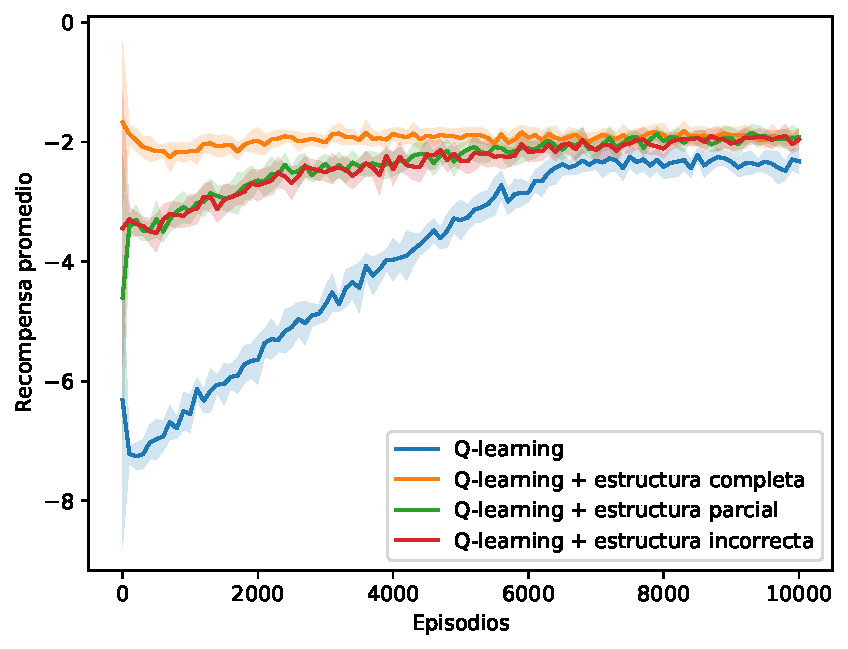
\includegraphics[width=.32\linewidth]{Chapter5/Figs/exp1/low/comparison_10_5_one_to_one_10000_deterministic_eps_partition_50.pdf}&
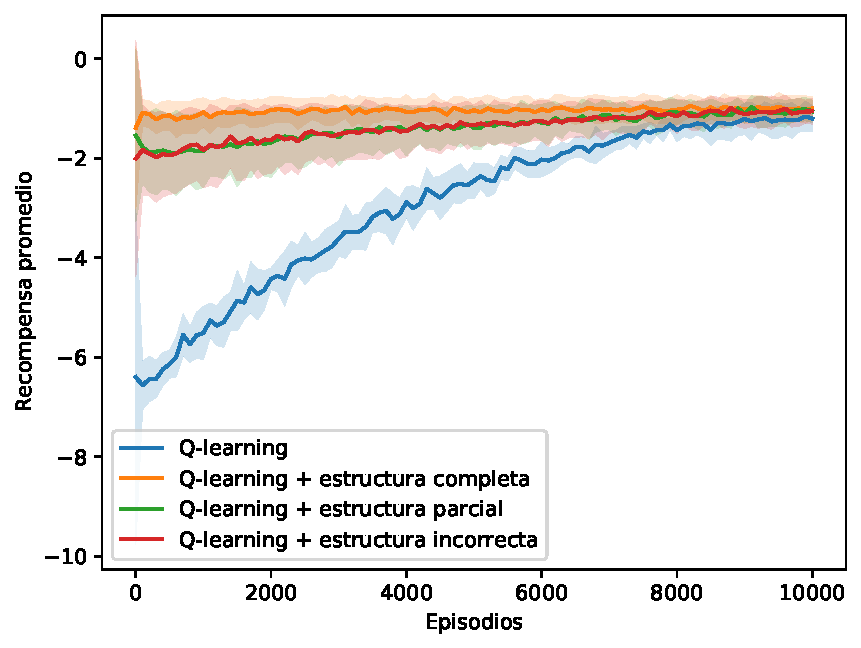
\includegraphics[width=.32\linewidth]{Chapter5/Figs/exp1/low/comparison_10_5_one_to_many_10000_deterministic_eps_partition_50.pdf}&
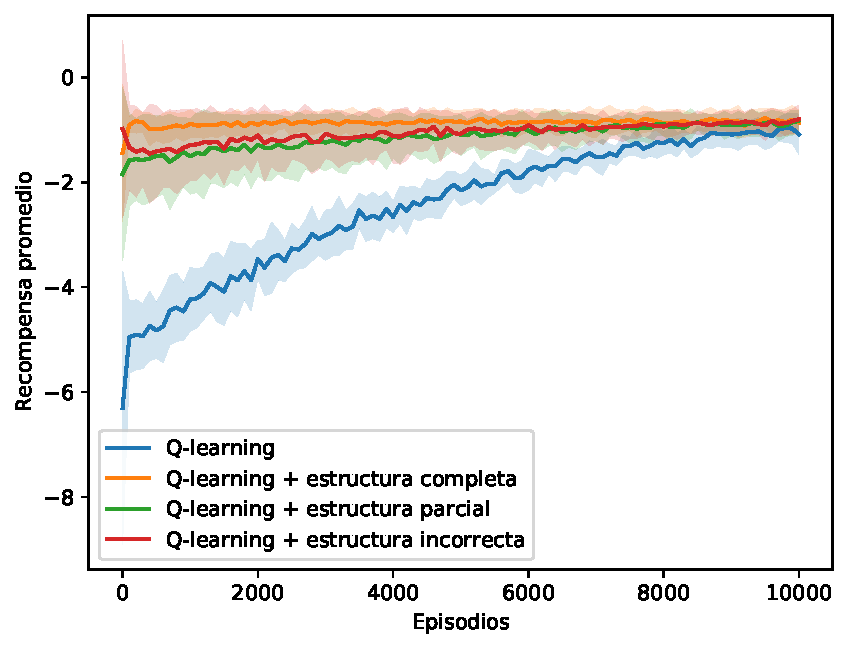
\includegraphics[width=.32\linewidth]{Chapter5/Figs/exp1/low/comparison_10_5_many_to_one_10000_deterministic_eps_partition_50.pdf}
\\
\rowname{$N=7$}&
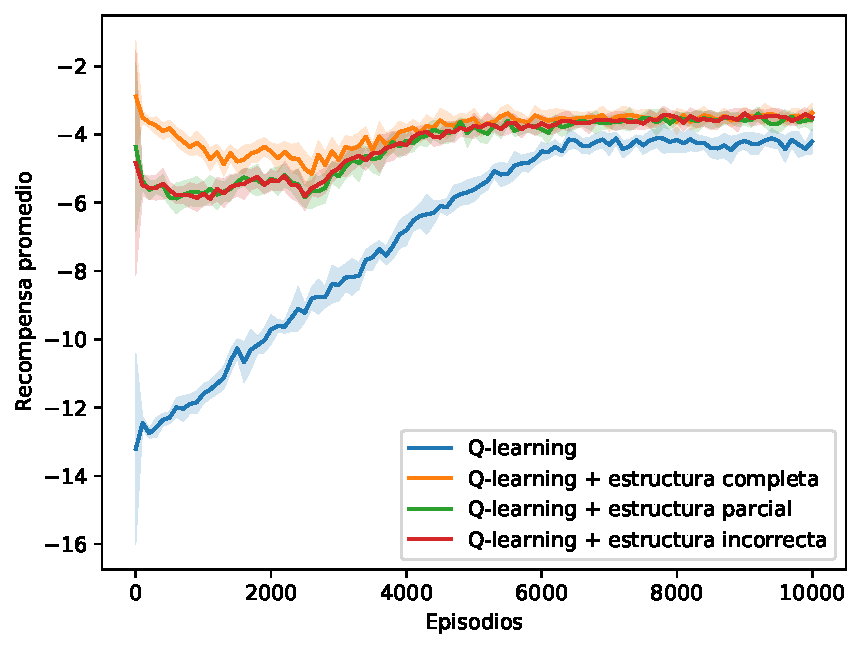
\includegraphics[width=.32\linewidth]{Chapter5/Figs/exp1/low/comparison_10_7_one_to_one_10000_deterministic_eps_partition_50.pdf}&
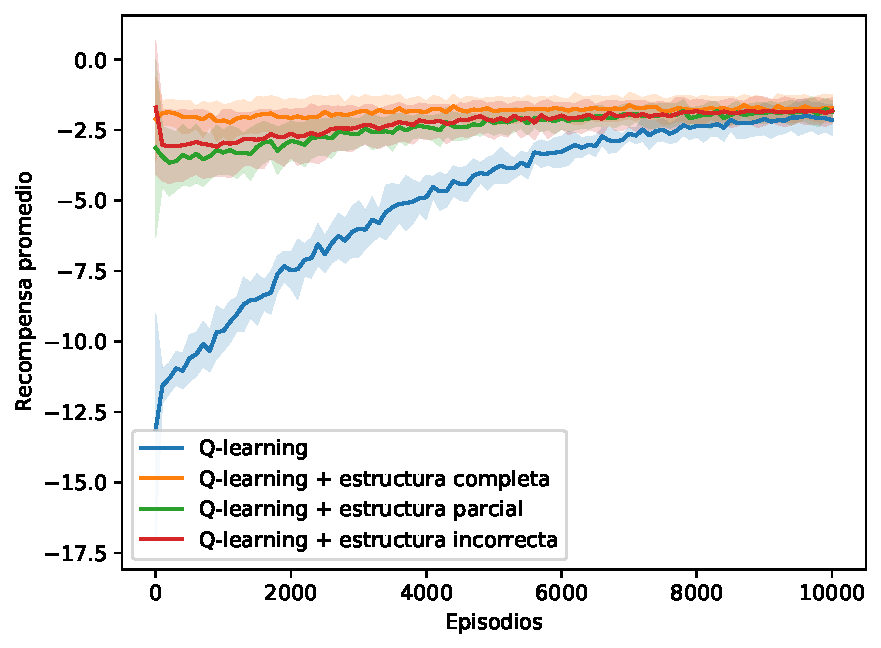
\includegraphics[width=.32\linewidth]{Chapter5/Figs/exp1/low/comparison_10_7_one_to_many_10000_deterministic_eps_partition_50.pdf}&
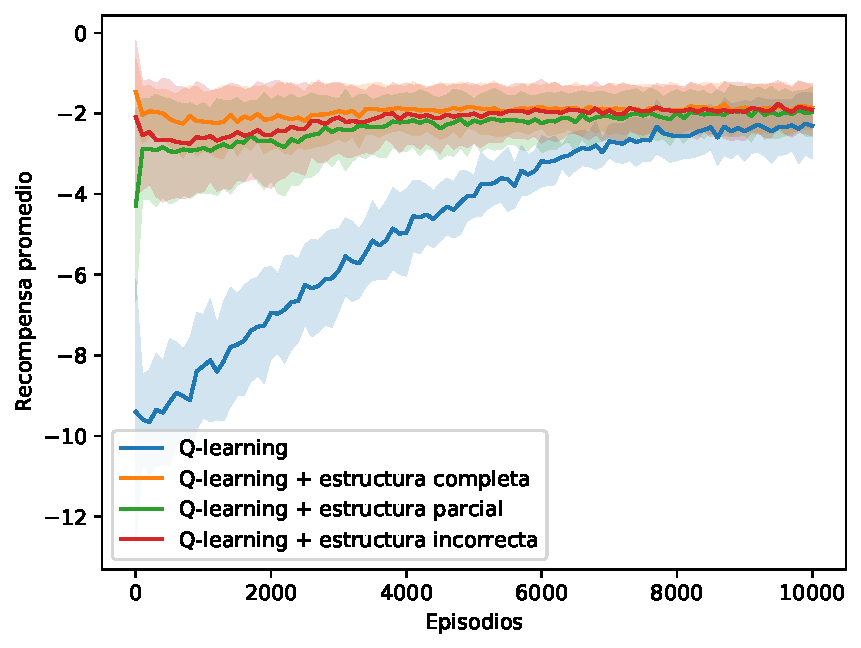
\includegraphics[width=.32\linewidth]{Chapter5/Figs/exp1/low/comparison_10_7_many_to_one_10000_deterministic_eps_partition_50.pdf}\\
\rowname{$N = 9$}&
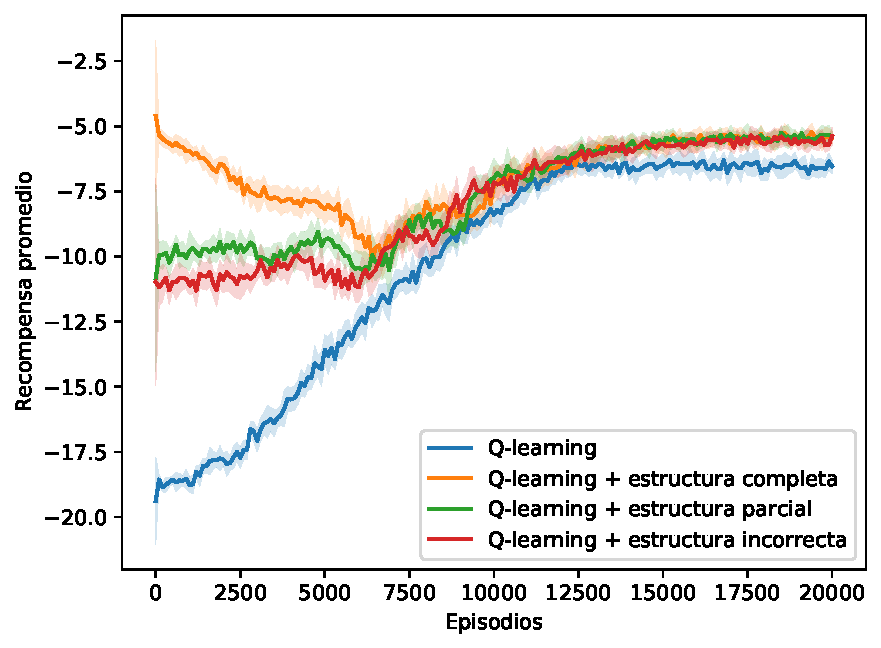
\includegraphics[width=.32\linewidth]{Chapter5/Figs/exp1/low/comparison_10_9_one_to_one_20000_deterministic_eps_partition_50.pdf}&
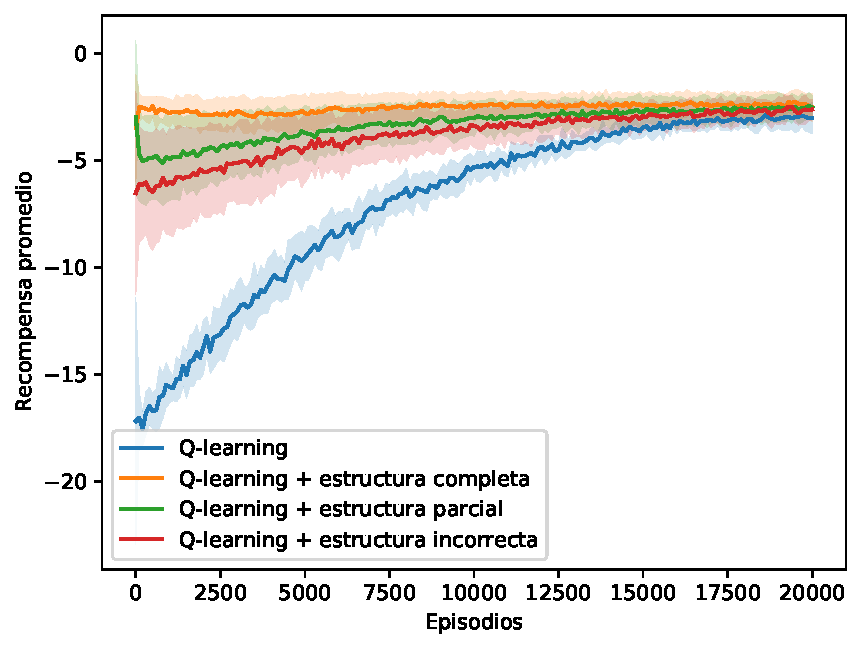
\includegraphics[width=.32\linewidth]{Chapter5/Figs/exp1/low/comparison_10_9_one_to_many_20000_deterministic_eps_partition_50.pdf}&
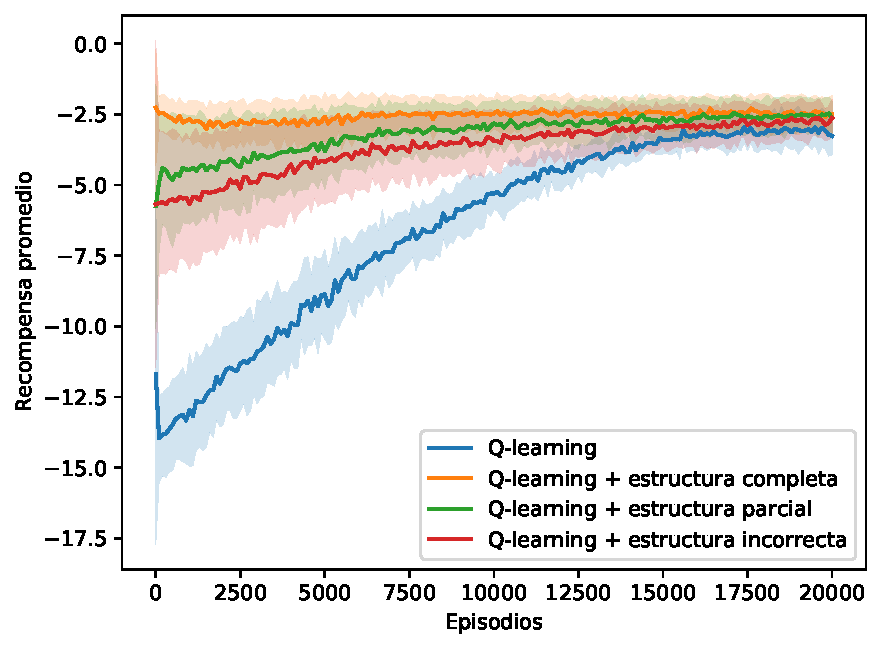
\includegraphics[width=.32\linewidth]{Chapter5/Figs/exp1/low/comparison_10_9_many_to_one_20000_deterministic_eps_partition_50.pdf}

\end{tabular}
\caption{Comparación del desempeño para los 4 algoritmos con un nivel de alteración $p_{mod} = 25 \%$ en un ambiente determinista. Las gráficas muestran la medida $average$ y la desviación estándar (región sombreada) para 10 experimentos.}
\label{fig:low-mod-det}
\end{figure}

\begin{figure}
\settoheight{\tempdima}{\includegraphics[width=.32\linewidth]{example-image-a}}%
\centering\begin{tabular}{@{}c@{ }c@{ }c@{ }c@{}}
&\textbf{Uno-a-uno} & \textbf{Causa común} & \textbf{Efecto común} \\
\rowname{$N = 5$}&
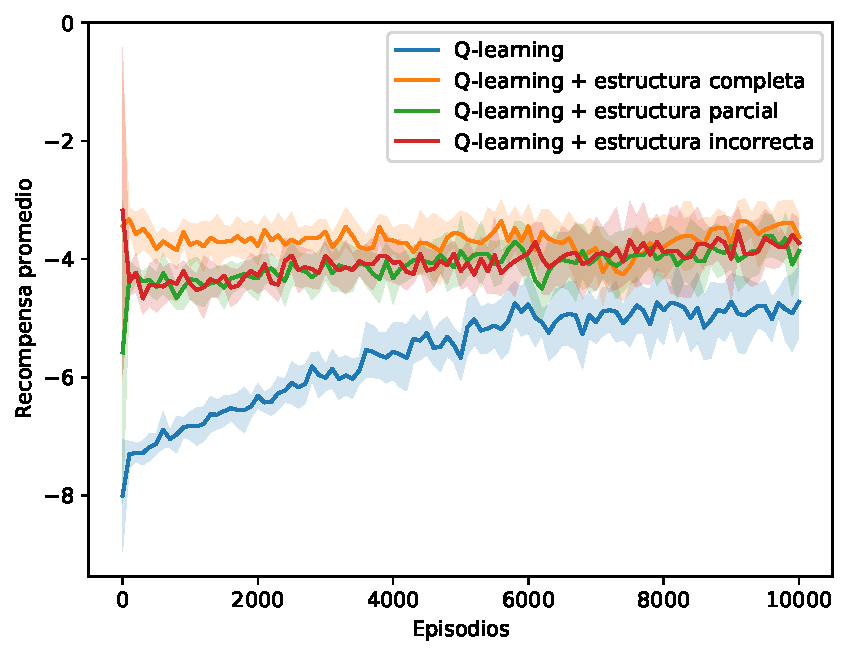
\includegraphics[width=.32\linewidth]{Chapter5/Figs/exp1/low/comparison_10_5_one_to_one_10000_stochastic_eps_partition_50.pdf}&
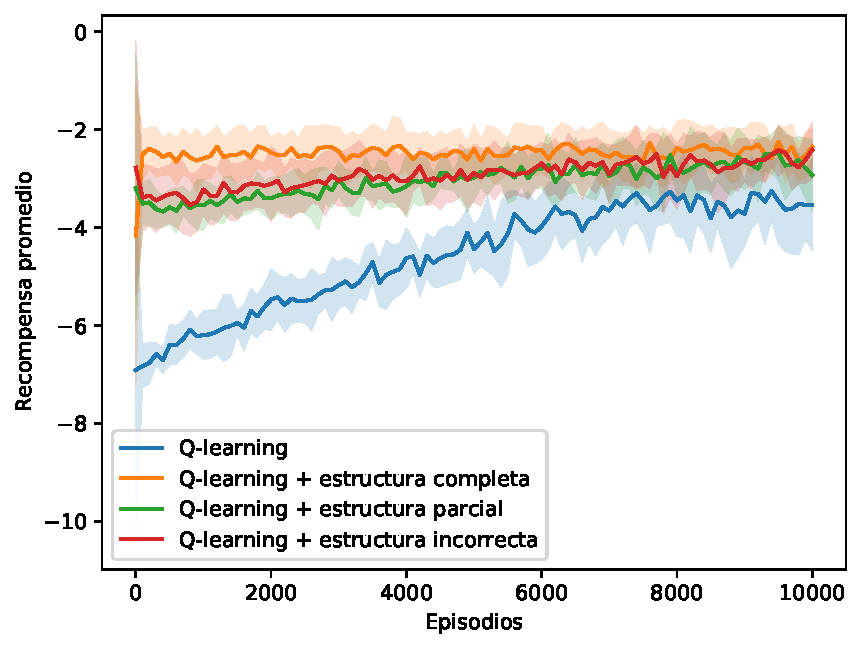
\includegraphics[width=.32\linewidth]{Chapter5/Figs/exp1/low/comparison_10_5_one_to_many_10000_stochastic_eps_partition_50.pdf}&
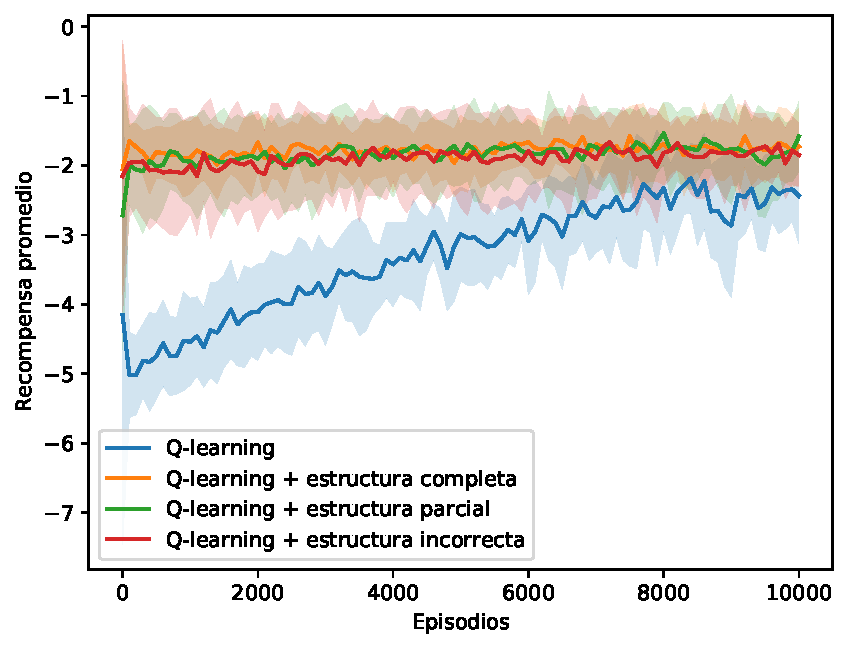
\includegraphics[width=.32\linewidth]{Chapter5/Figs/exp1/low/comparison_10_5_many_to_one_10000_stochastic_eps_partition_50.pdf}\\
\rowname{$N=7$}&
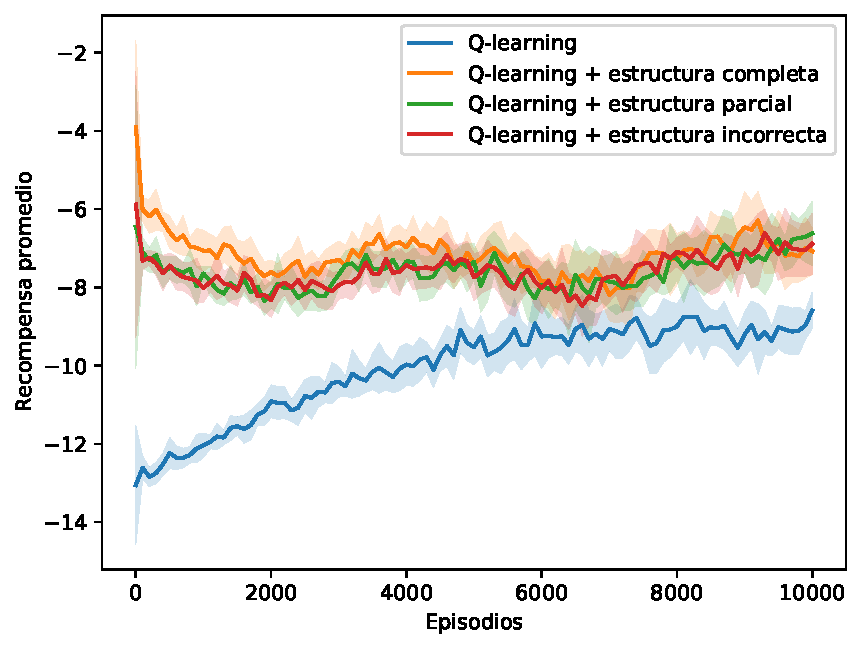
\includegraphics[width=.32\linewidth]{Chapter5/Figs/exp1/low/comparison_10_7_one_to_one_10000_stochastic_eps_partition_50.pdf}&
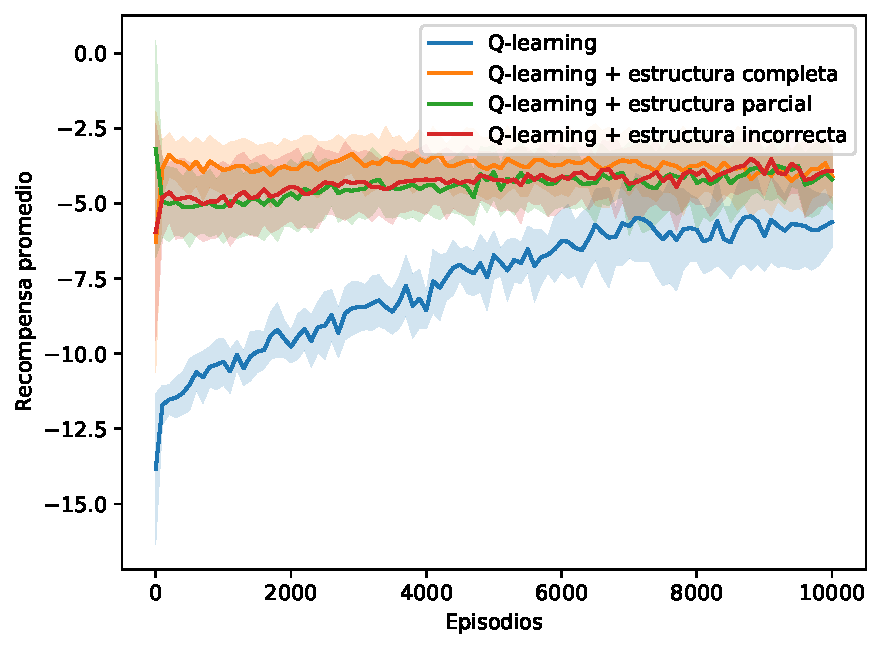
\includegraphics[width=.32\linewidth]{Chapter5/Figs/exp1/low/comparison_10_7_one_to_many_10000_stochastic_eps_partition_50.pdf}&
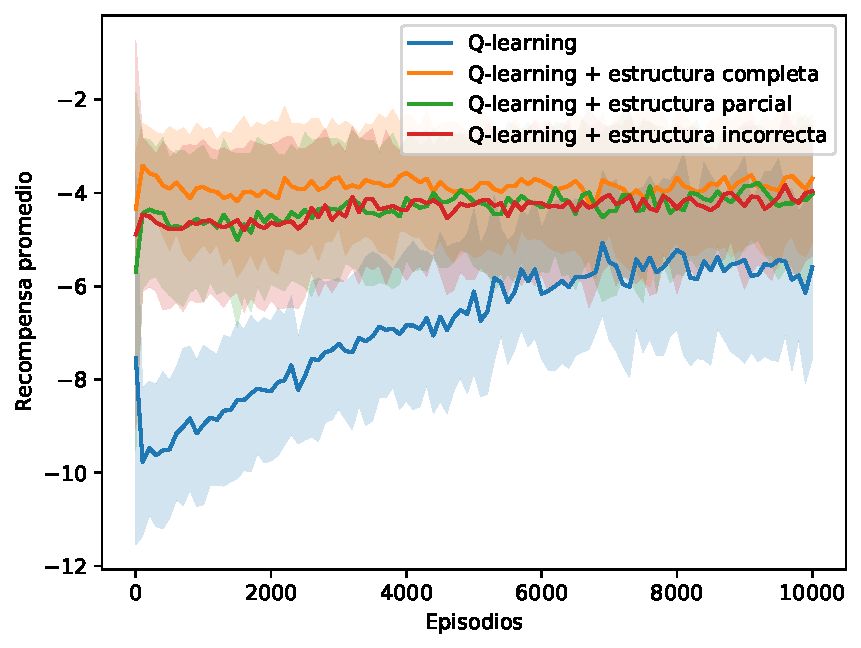
\includegraphics[width=.32\linewidth]{Chapter5/Figs/exp1/low/comparison_10_7_many_to_one_10000_stochastic_eps_partition_50.pdf}\\
\rowname{$N = 9$}&
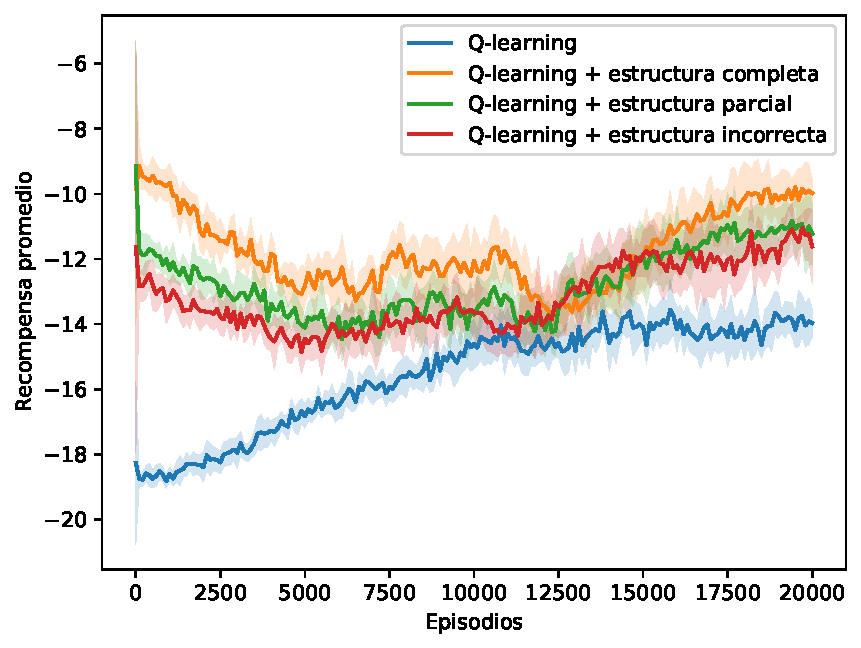
\includegraphics[width=.32\linewidth]{Chapter5/Figs/exp1/low/comparison_10_9_one_to_one_20000_stochastic_eps_partition_50.pdf}&
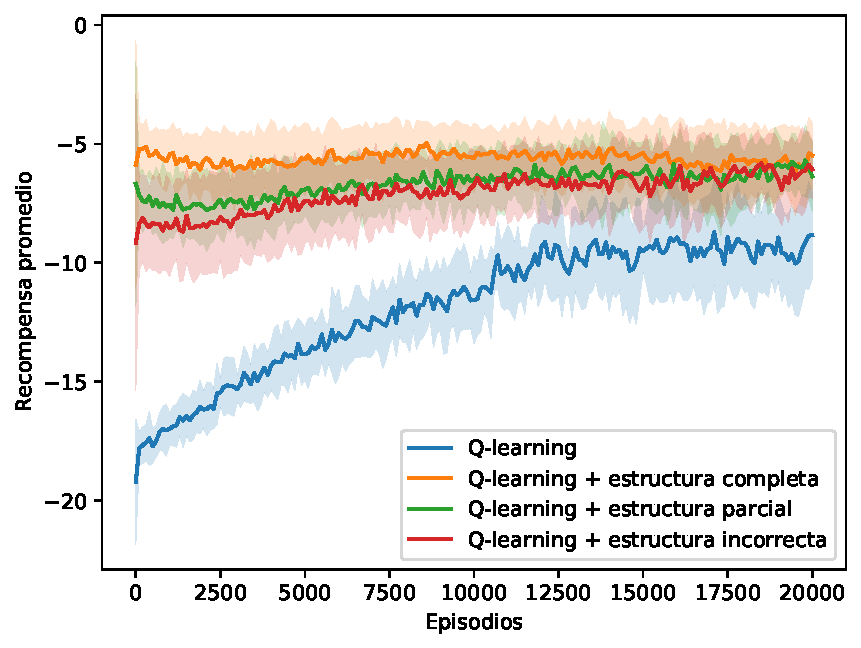
\includegraphics[width=.32\linewidth]{Chapter5/Figs/exp1/low/comparison_10_9_one_to_many_20000_stochastic_eps_partition_50.pdf}&
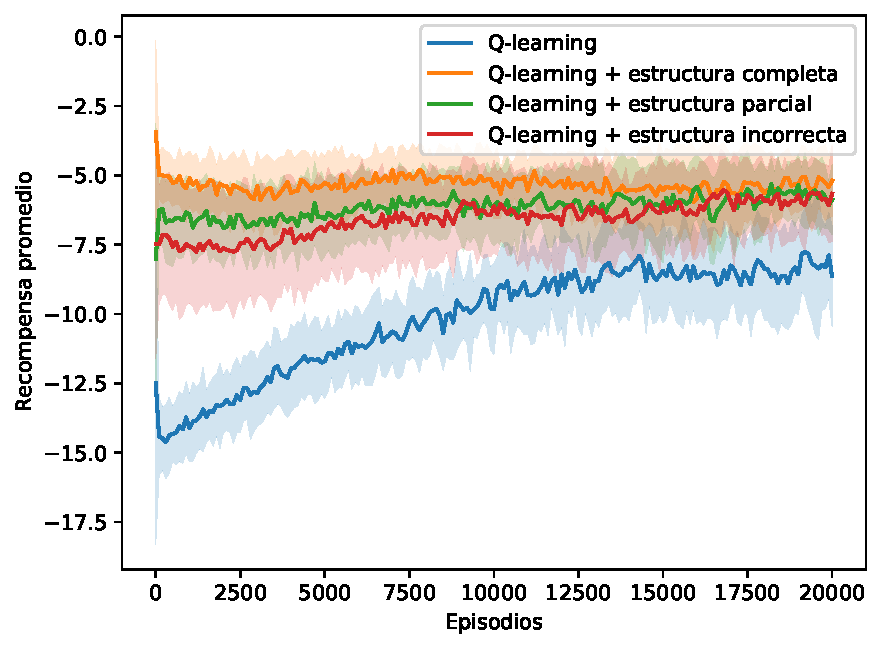
\includegraphics[width=.32\linewidth]{Chapter5/Figs/exp1/low/comparison_10_9_many_to_one_20000_stochastic_eps_partition_50.pdf}

\end{tabular}
\caption{Comparación del desempeño para los 4 algoritmos con un nivel de alteración $p_{mod} = 25 \%$ en un ambiente estocástico. Las gráficas muestran la medida $average$ y la desviación estándar (región sombreada) para 10 experimentos.}
\label{fig:low-mod-sto}
\end{figure}


\begin{figure}
\settoheight{\tempdima}{\includegraphics[width=.32\linewidth]{example-image-a}}%
\centering\begin{tabular}{@{}c@{ }c@{ }c@{ }c@{}}
&\textbf{Uno-a-uno} & \textbf{Causa común} & \textbf{Efecto común} \\
\rowname{$N = 5$}&
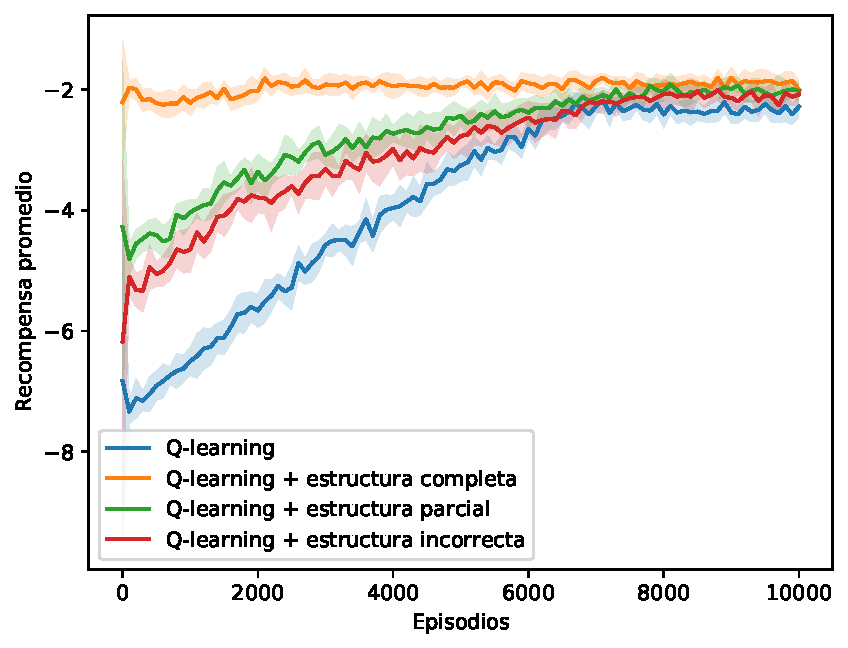
\includegraphics[width=.32\linewidth]{Chapter5/Figs/exp1/medium/comparison_10_5_one_to_one_10000_deterministic_eps_partition_50.pdf}&
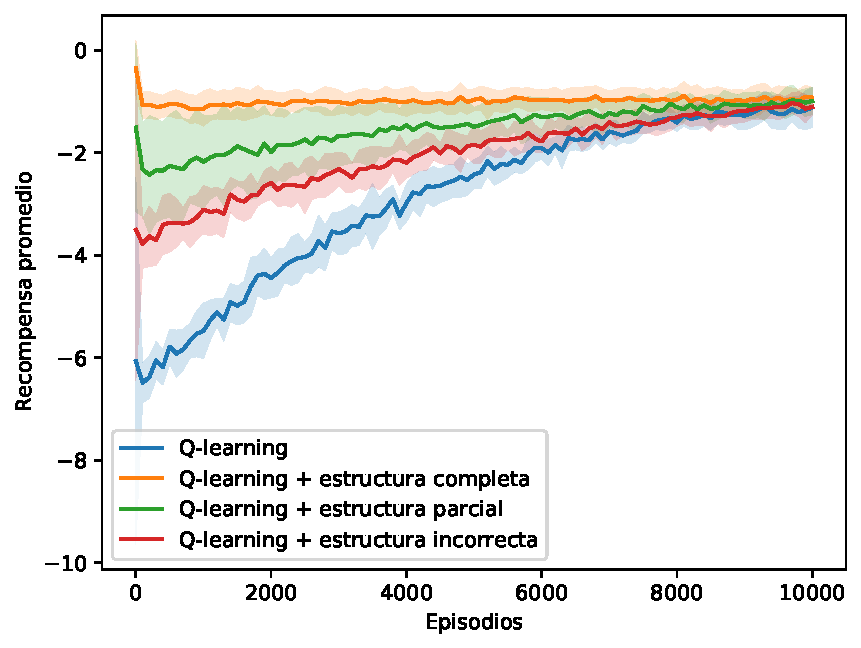
\includegraphics[width=.32\linewidth]{Chapter5/Figs/exp1/medium/comparison_10_5_one_to_many_10000_deterministic_eps_partition_50.pdf}&
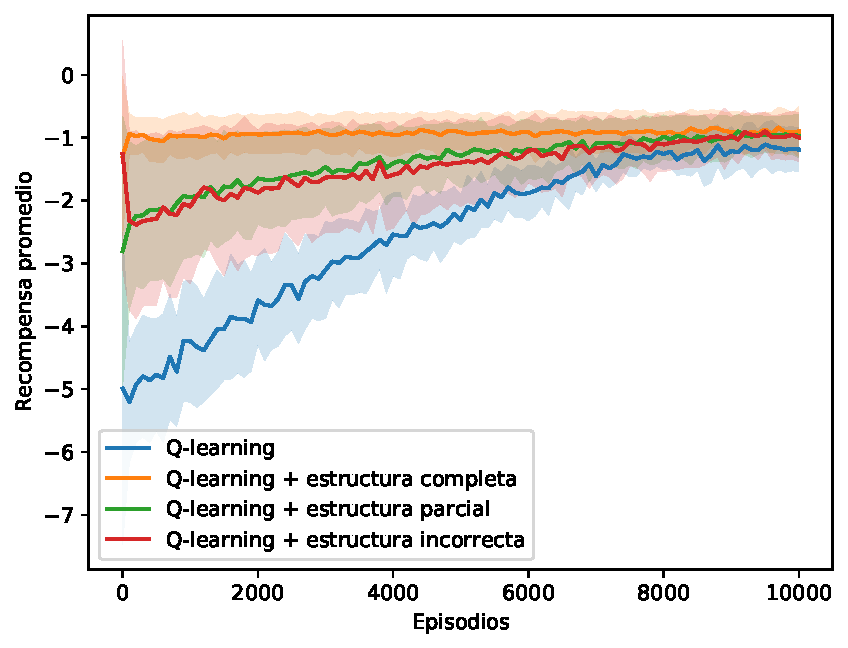
\includegraphics[width=.32\linewidth]{Chapter5/Figs/exp1/medium/comparison_10_5_many_to_one_10000_deterministic_eps_partition_50.pdf}\\
\rowname{$N=7$}&
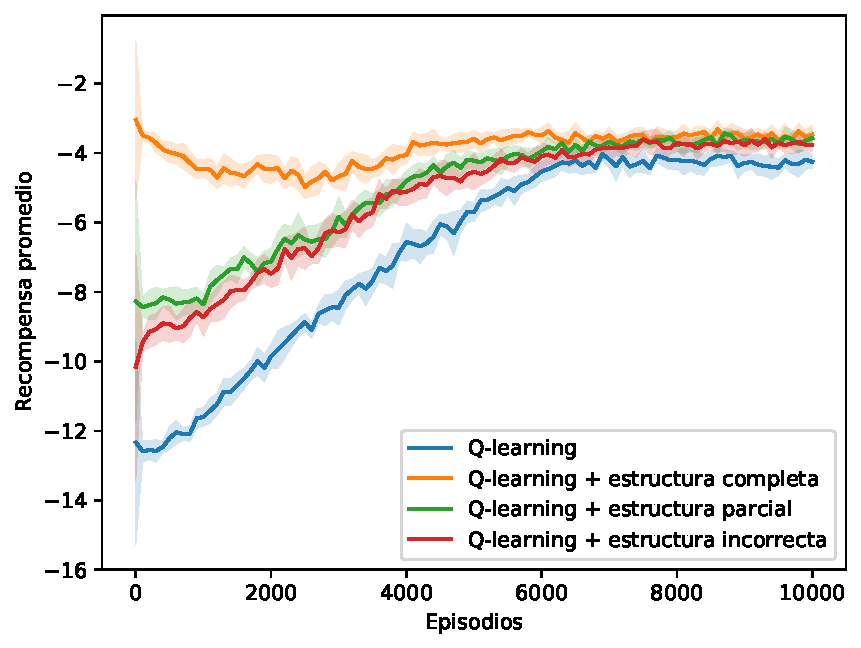
\includegraphics[width=.32\linewidth]{Chapter5/Figs/exp1/medium/comparison_10_7_one_to_one_10000_deterministic_eps_partition_50.pdf}&
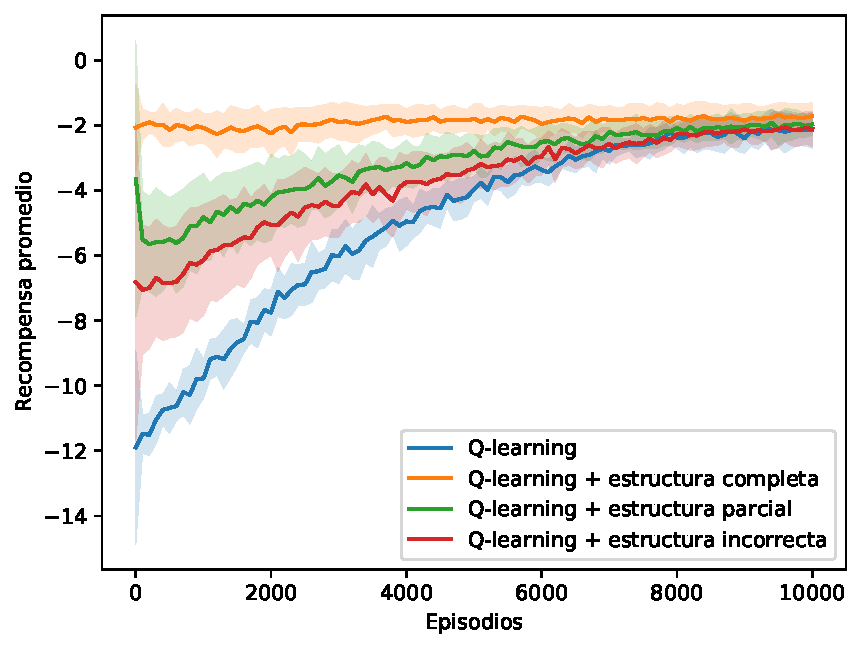
\includegraphics[width=.32\linewidth]{Chapter5/Figs/exp1/medium/comparison_10_7_one_to_many_10000_deterministic_eps_partition_50.pdf}&
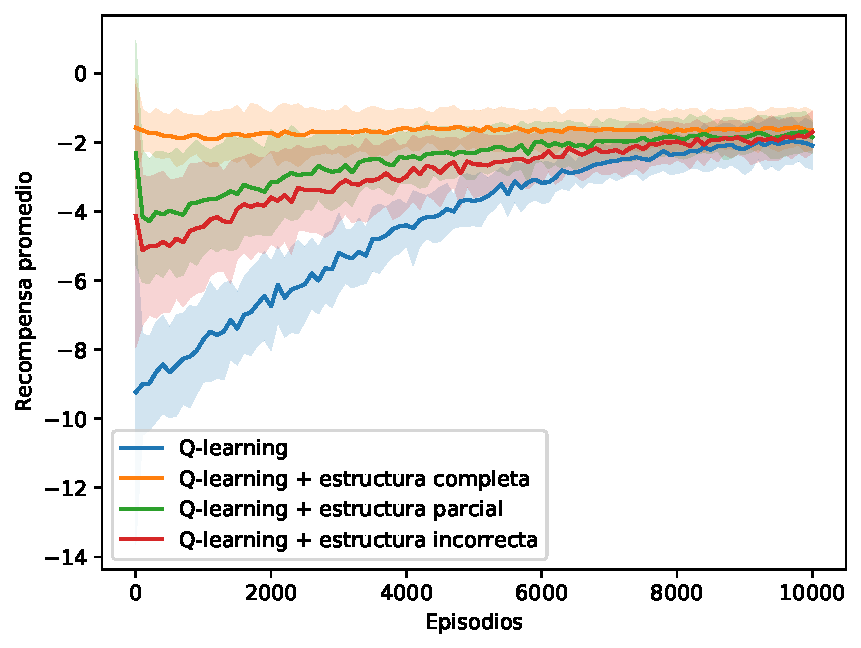
\includegraphics[width=.32\linewidth]{Chapter5/Figs/exp1/medium/comparison_10_7_many_to_one_10000_deterministic_eps_partition_50.pdf}\\
\rowname{$N = 9$}&
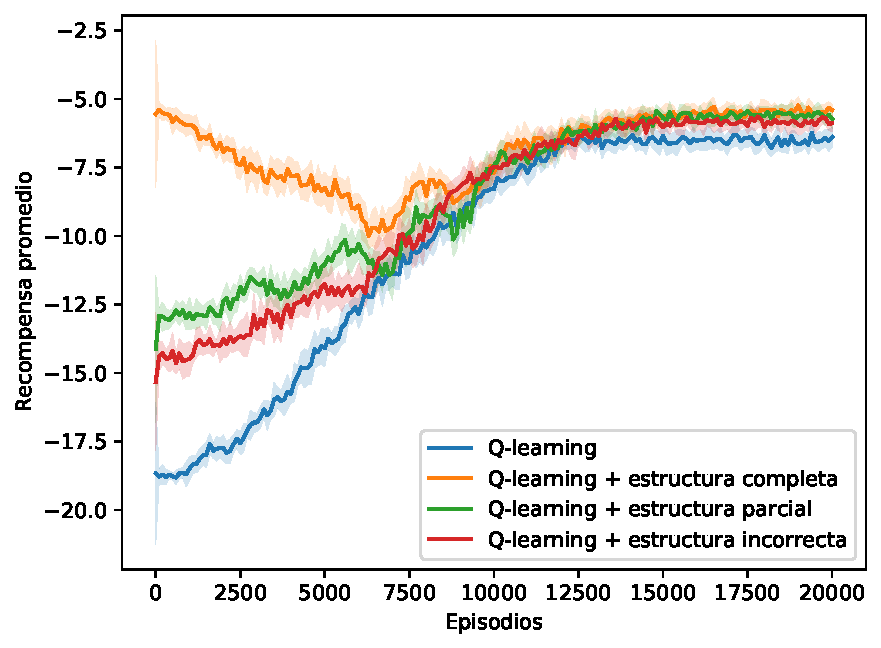
\includegraphics[width=.32\linewidth]{Chapter5/Figs/exp1/medium/comparison_10_9_one_to_one_20000_deterministic_eps_partition_50.pdf}&
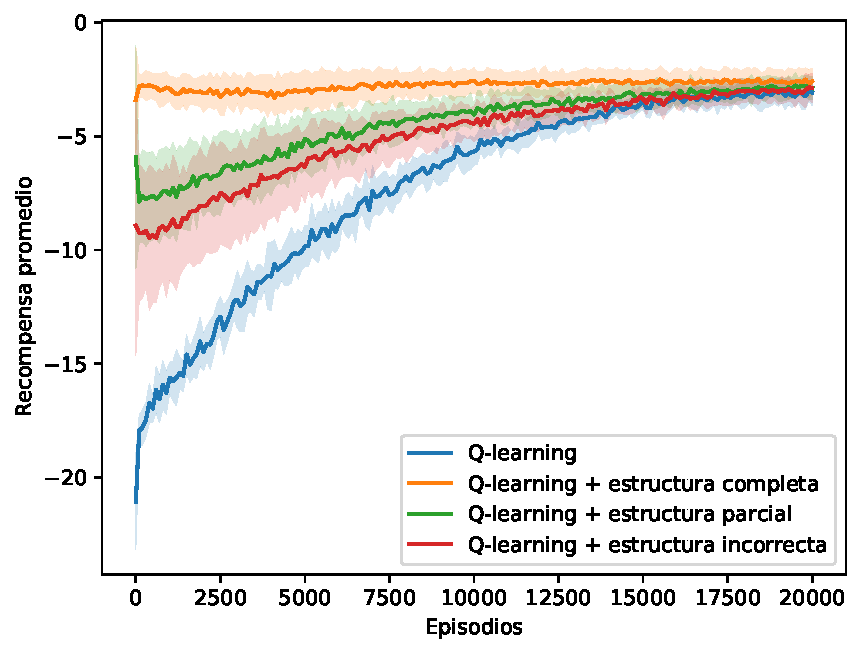
\includegraphics[width=.32\linewidth]{Chapter5/Figs/exp1/medium/comparison_10_9_one_to_many_20000_deterministic_eps_partition_50.pdf}&
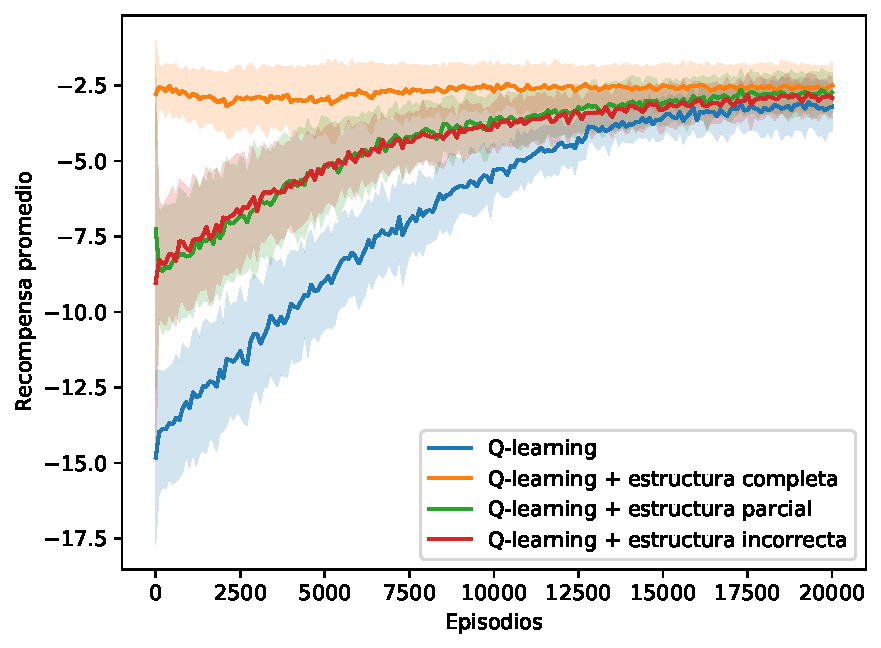
\includegraphics[width=.32\linewidth]{Chapter5/Figs/exp1/medium/comparison_10_9_many_to_one_20000_deterministic_eps_partition_50.pdf}

\end{tabular}
\caption{Comparación del desempeño para los 4 algoritmos con un nivel de alteración $p_{mod} = 50 \%$ en un ambiente determinista. Las gráficas muestran la medida $average$ y la desviación estándar (región sombreada) para 10 experimentos.}
\label{fig:med-mod-det}
\end{figure}

% \begin{figure}
% \settoheight{\tempdima}{\includegraphics[width=.32\linewidth]{example-image-a}}%
% \centering\begin{tabular}{@{}c@{ }c@{ }c@{ }c@{}}
% &\textbf{Uno-a-uno} & \textbf{Causa común} & \textbf{Efecto común} \\
% \rowname{$N = 5$}&
% \includegraphics[width=.32\linewidth]{example-image-a}&
% \includegraphics[width=.32\linewidth]{example-image-b}&
% \includegraphics[width=.32\linewidth]{example-image-c}\\
% \rowname{$N=7$}&
% \includegraphics[width=.32\linewidth]{example-image-a}&
% \includegraphics[width=.32\linewidth]{example-image-b}&
% \includegraphics[width=.32\linewidth]{example-image-c}\\
% \rowname{$N = 9$}&
% \includegraphics[width=.32\linewidth]{example-image-a}&
% \includegraphics[width=.32\linewidth]{example-image-b}&
% \includegraphics[width=.32\linewidth]{example-image-c}

% \end{tabular}
% \caption{Comparación del desempeño para los 4 algoritmos con un nivel de alteración $p_{mod} = 50 \%$ en un ambiente estocástico. Las gráficas muestran la medida $average$ y la desviación estándar (región sombreada) para 10 experimentos.}
% \label{fig:med-mod-sto}
% \end{figure}


\begin{figure}
\settoheight{\tempdima}{\includegraphics[width=.32\linewidth]{example-image-a}}%
\centering\begin{tabular}{@{}c@{ }c@{ }c@{ }c@{}}
&\textbf{Uno-a-uno} & \textbf{Causa común} & \textbf{Efecto común} \\
\rowname{$N = 5$}&
\includegraphics[width=.32\linewidth]{Chapter5/Figs/exp1/high/comparison_10_5_one_to_one_10000_deterministic_eps_partition_50.pdf}&
\includegraphics[width=.32\linewidth]{Chapter5/Figs/exp1/high/comparison_10_5_one_to_many_10000_deterministic_eps_partition_50.pdf}&
\includegraphics[width=.32\linewidth]{Chapter5/Figs/exp1/high/comparison_10_5_many_to_one_10000_deterministic_eps_partition_50.pdf}\\
\rowname{$N=7$}&
\includegraphics[width=.32\linewidth]{Chapter5/Figs/exp1/high/comparison_10_7_one_to_one_10000_deterministic_eps_partition_50.pdf}&
\includegraphics[width=.32\linewidth]{Chapter5/Figs/exp1/high/comparison_10_7_one_to_many_10000_deterministic_eps_partition_50.pdf}&
\includegraphics[width=.32\linewidth]{Chapter5/Figs/exp1/high/comparison_10_7_many_to_one_10000_deterministic_eps_partition_50.pdf}\\
\rowname{$N = 9$}&
\includegraphics[width=.32\linewidth]{Chapter5/Figs/exp1/high/comparison_10_9_one_to_one_20000_deterministic_eps_partition_50.pdf}&
\includegraphics[width=.32\linewidth]{Chapter5/Figs/exp1/high/comparison_10_9_one_to_many_20000_deterministic_eps_partition_50.pdf}&
\includegraphics[width=.32\linewidth]{Chapter5/Figs/exp1/high/comparison_10_9_many_to_one_20000_deterministic_eps_partition_50.pdf}

\end{tabular}
\caption{Comparación del desempeño para los 4 algoritmos con un nivel de alteración $p_{mod} = 75 \%$ en un ambiente determinista. Las gráficas muestran la medida $average$ y la desviación estándar (región sombreada) para 10 experimentos.}
\label{fig:high-mod-det}
\end{figure}

% \begin{figure}
% \settoheight{\tempdima}{\includegraphics[width=.32\linewidth]{example-image-a}}%
% \centering\begin{tabular}{@{}c@{ }c@{ }c@{ }c@{}}
% &\textbf{Uno-a-uno} & \textbf{Causa común} & \textbf{Efecto común} \\
% \rowname{$N = 5$}&
% \includegraphics[width=.32\linewidth]{example-image-a}&
% \includegraphics[width=.32\linewidth]{example-image-b}&
% \includegraphics[width=.32\linewidth]{example-image-c}\\
% \rowname{$N=7$}&
% \includegraphics[width=.32\linewidth]{example-image-a}&
% \includegraphics[width=.32\linewidth]{example-image-b}&
% \includegraphics[width=.32\linewidth]{example-image-c}\\
% \rowname{$N = 9$}&
% \includegraphics[width=.32\linewidth]{example-image-a}&
% \includegraphics[width=.32\linewidth]{example-image-b}&
% \includegraphics[width=.32\linewidth]{example-image-c}

% \end{tabular}
% \caption{Comparación del desempeño para los 4 algoritmos con un nivel de alteración $p_{mod} = 75 \%$ en un ambiente estocástico. Las gráficas muestran la medida $average$ y la desviación estándar (región sombreada) para 10 experimentos.}
% \label{fig:high-mod-sto}
% \end{figure}


\newpage

\subsection{Explotar o seguir explorando}\label{subsection:exp-epsilon}


\begin{itemize}
    \item El espacio de estados es discreto, es decir, el agente puede
    obtener las variables $\mathcal{X}$ directamente del ambiente.
    \item Para obtener a los
    grafos $\mathcal{D'}$ y $\mathcal{D''}$,
    el porcentaje de nivel de cambio  es $p_{mod} = 25 \%$. Esto significa que no se altera demasiado el grafo causal original para
    generar los grafos incompletos e incorrectos.
    \item Se controla qué tan rápido se desea alcanzar $\epsilon_{\min}$ variando el parámetro $\delta$. Si se divide al entrenamiento en cuartos,  entonces los valores de $\delta$ corresponden a en qué cuarto se alcanza el mínimo valor para $\epsilon$.
    \begin{itemize}
        \item Alcanzar $\epsilon_{\min}$ en el primer cuarto del entrenamiento, $\delta = 0.25$.
        \item Alcanzar $\epsilon_{\min}$ a medio aprendizaje, $\delta = 0.50$.
        \item Alcanzar $\epsilon_{\min}$ en el tercer cuarto del entrenamiento, $\delta = 0.75$.
    \end{itemize}
    \item Se examina sobre los tres tipos de estructuras posibles: uno-a-uno, 
    causa común y efecto común. 
    \item Se prueba sobre un mundo determinista.
\end{itemize}

\subsubsection{Objetivo}

Determinar si reducir o aumentar las consultas al grafo causal a lo largo del aprendizaje afecta el desempeño
de los algoritmos.

\subsubsection{Hipótesis}

La información del grafo causal no afecta negativamente 
el aprendizaje de la función de valor $Q$. Por lo tanto, incluso si se disminuyen las consultas al modelo de manera temprana en el entrenamiento, la información provista habrá
ayudado al aprendizaje de la función.

\subsubsection{Resultados}

En las Figuras \ref{fig:low-epsilon-det} y \ref{fig:high-epsilon-det} se puede ver que los algoritmos que utilizan conocimiento del grafo inician con una recompensa mayor y se estabilizan más rápido que el algoritmo Q-learning
sin información adicional en ambientes con transiciones deterministas. 
De acuerdo con los resultados parece que 
entre mayor sea $\delta$ más tarda en estabilizarse
el algoritmo de aprendizaje sin información que lo auxilie. Esto es de esperarse, ya que se sigue explorando durante más tiempo. Sin embargo,
también se puede notar que estimula a dejar
la exploración de manera temprana, no implica que después
de dejarla, el algoritmo converge inmediatamente. Por otro lado, 
la recompensa, en los algoritmos que se guían por el grafo, se desestabiliza
el intervalo en el que se encuentra la transición a dejar de dar peso a 
la exploración. Pero, una vez fuera de esa ``zona de transición'' los
algoritmos se recuperan y tienden a estar por encima del algoritmo sin datos 
extra.


\begin{figure}
\settoheight{\tempdima}{\includegraphics[width=.32\linewidth]{example-image-a}}%
\centering\begin{tabular}{@{}c@{ }c@{ }c@{ }c@{}}
&\textbf{Uno-a-uno} & \textbf{Causa común} & \textbf{Efecto común} \\
\rowname{$N = 5$}&
\includegraphics[width=.32\linewidth]{Chapter5/Figs/exp2/low/comparison_10_5_one_to_one_5000_deterministic_eps_partition_25.pdf}&
\includegraphics[width=.32\linewidth]{Chapter5/Figs/exp2/low/comparison_10_5_one_to_many_5000_deterministic_eps_partition_25.pdf}&
\includegraphics[width=.32\linewidth]{Chapter5/Figs/exp2/low/comparison_10_5_many_to_one_5000_deterministic_eps_partition_25.pdf}\\
\rowname{$N=7$}&
\includegraphics[width=.32\linewidth]{Chapter5/Figs/exp2/low/comparison_10_7_one_to_one_5000_deterministic_eps_partition_25.pdf}&
\includegraphics[width=.32\linewidth]{Chapter5/Figs/exp2/low/comparison_10_7_one_to_many_5000_deterministic_eps_partition_25.pdf}&
\includegraphics[width=.32\linewidth]{Chapter5/Figs/exp2/low/comparison_10_7_many_to_one_5000_deterministic_eps_partition_25.pdf}\\
\rowname{$N = 9$}&
\includegraphics[width=.32\linewidth]{Chapter5/Figs/exp2/low/comparison_10_9_one_to_one_10000_deterministic_eps_partition_25.pdf}&
\includegraphics[width=.32\linewidth]{Chapter5/Figs/exp2/low/comparison_10_9_one_to_many_10000_deterministic_eps_partition_25.pdf}&
\includegraphics[width=.32\linewidth]{Chapter5/Figs/exp2/low/comparison_10_9_many_to_one_10000_deterministic_eps_partition_25.pdf}
\end{tabular}
\caption{Comparación del desempeño para los 4 algoritmos con un nivel de alteración $p_{mod} = 25 \%$  y $\delta = 0.25$ en un ambiente determinista. Las gráficas muestran la medida $average$ y la desviación estándar (región sombreada) para 10 experimentos.}
\label{fig:low-epsilon-det}
\end{figure}

% \begin{figure}
% \settoheight{\tempdima}{\includegraphics[width=.32\linewidth]{example-image-a}}%
% \centering\begin{tabular}{@{}c@{ }c@{ }c@{ }c@{}}
% &\textbf{Uno-a-uno} & \textbf{Causa común} & \textbf{Efecto común} \\
% \rowname{$N = 5$}&
% \includegraphics[width=.32\linewidth]{example-image-a}&
% \includegraphics[width=.32\linewidth]{example-image-b}&
% \includegraphics[width=.32\linewidth]{example-image-c}\\
% \rowname{$N=7$}&
% \includegraphics[width=.32\linewidth]{example-image-a}&
% \includegraphics[width=.32\linewidth]{example-image-b}&
% \includegraphics[width=.32\linewidth]{example-image-c}\\
% \rowname{$N = 9$}&
% \includegraphics[width=.32\linewidth]{example-image-a}&
% \includegraphics[width=.32\linewidth]{example-image-b}&
% \includegraphics[width=.32\linewidth]{example-image-c}

% \end{tabular}
% \caption{Comparación del desempeño para los 4 algoritmos con un nivel de alteración $p_{mod} = 75 \%$ en un ambiente estocástico. Las gráficas muestran la medida $average$ y la desviación estándar (región sombreada) para 10 experimentos.}
% \label{fig:low-epsilon-sto}
% \end{figure}

\begin{figure}
\settoheight{\tempdima}{\includegraphics[width=.32\linewidth]{example-image-a}}%
\centering\begin{tabular}{@{}c@{ }c@{ }c@{ }c@{}}
&\textbf{Uno-a-uno} & \textbf{Causa común} & \textbf{Efecto común} \\
\rowname{$N = 5$}&
\includegraphics[width=.32\linewidth]{example-image-a}&
\includegraphics[width=.32\linewidth]{Chapter5/Figs/exp2/high/comparison_10_5_one_to_many_5000_deterministic_eps_partition_75.pdf}&
\includegraphics[width=.32\linewidth]{Chapter5/Figs/exp2/high/comparison_10_5_many_to_one_5000_deterministic_eps_partition_75.pdf}\\
\rowname{$N=7$}&
\includegraphics[width=.32\linewidth]{example-image-a}&
\includegraphics[width=.32\linewidth]{Chapter5/Figs/exp2/high/comparison_10_7_one_to_many_5000_deterministic_eps_partition_75.pdf}&
\includegraphics[width=.32\linewidth]{Chapter5/Figs/exp2/high/comparison_10_7_many_to_one_5000_deterministic_eps_partition_75.pdf}\\
\rowname{$N = 9$}&
\includegraphics[width=.32\linewidth]{example-image-a}&
\includegraphics[width=.32\linewidth]{Chapter5/Figs/exp2/high/comparison_10_9_one_to_many_10000_deterministic_eps_partition_75.pdf}&
\includegraphics[width=.32\linewidth]{Chapter5/Figs/exp2/high/comparison_10_9_many_to_one_10000_deterministic_eps_partition_75.pdf}
\end{tabular}
\caption{Comparación del desempeño para los 4 algoritmos con un nivel de alteración $p_{mod} = 25 \%$ y $\delta = 0.75$ en un ambiente determinista. Las gráficas muestran la medida $average$ y la desviación estándar (región sombreada) para 10 experimentos.}
\label{fig:high-epsilon-det}
\end{figure}

% \begin{figure}
% \settoheight{\tempdima}{\includegraphics[width=.32\linewidth]{example-image-a}}%
% \centering\begin{tabular}{@{}c@{ }c@{ }c@{ }c@{}}
% &\textbf{Uno-a-uno} & \textbf{Causa común} & \textbf{Efecto común} \\
% \rowname{$N = 5$}&
% \includegraphics[width=.32\linewidth]{example-image-a}&
% \includegraphics[width=.32\linewidth]{example-image-b}&
% \includegraphics[width=.32\linewidth]{example-image-c}\\
% \rowname{$N=7$}&
% \includegraphics[width=.32\linewidth]{example-image-a}&
% \includegraphics[width=.32\linewidth]{example-image-b}&
% \includegraphics[width=.32\linewidth]{example-image-c}\\
% \rowname{$N = 9$}&
% \includegraphics[width=.32\linewidth]{example-image-a}&
% \includegraphics[width=.32\linewidth]{example-image-b}&
% \includegraphics[width=.32\linewidth]{example-image-c}

% \end{tabular}
% \caption{Comparación del desempeño para los 4 algoritmos con un nivel de alteración $p_{mod} = 75 \%$ en un ambiente estocástico. Las gráficas muestran la medida $average$ y la desviación estándar (región sombreada) para 10 experimentos.}
% \label{fig:med-epsilon-sto}
% \end{figure}

% \begin{figure}
% \settoheight{\tempdima}{\includegraphics[width=.32\linewidth]{example-image-a}}%
% \centering\begin{tabular}{@{}c@{ }c@{ }c@{ }c@{}}
% &\textbf{Uno-a-uno} & \textbf{Causa común} & \textbf{Efecto común} \\
% \rowname{$N = 5$}&
% \includegraphics[width=.32\linewidth]{example-image-a}&
% \includegraphics[width=.32\linewidth]{example-image-b}&
% \includegraphics[width=.32\linewidth]{example-image-c}\\
% \rowname{$N=7$}&
% \includegraphics[width=.32\linewidth]{example-image-a}&
% \includegraphics[width=.32\linewidth]{example-image-b}&
% \includegraphics[width=.32\linewidth]{example-image-c}\\
% \rowname{$N = 9$}&
% \includegraphics[width=.32\linewidth]{example-image-a}&
% \includegraphics[width=.32\linewidth]{example-image-b}&
% \includegraphics[width=.32\linewidth]{example-image-c}

% \end{tabular}
% \caption{Comparación del desempeño para los 4 algoritmos con un nivel de alteración $p_{mod} = 75 \%$ en un ambiente estocástico. Las gráficas muestran la medida $average$ y la desviación estándar (región sombreada) para 10 experimentos.}
% \label{fig:high-epsilon-sto}
% \end{figure}

\newpage

\subsection{Utilizando observaciones visuales del ambiente}

\subsubsection{Configuración experimental}

\begin{itemize}
    \item Los elementos del espacio de estados $\mathcal{S}$, son continuos.
    Las observaciones son imágenes de $84\times 84$ pixeles en un espacio de color RGB, obtenidas desde una vista cenital del ambiente.
    
    \begin{figure}[H]
        \centering
        \includegraphics[scale=0.2]{Chapter5/Figs/obs_example.png}
        \caption{Ejemplo de una posible observación del agente.}
        \label{fig:obs-example-lights}
    \end{figure}
    \item Para mapear las imágenes al espacio de estados de alto nivel $\mathcal{X}$, la función $\phi$ es un clasificador multi etiqueta
    parametrizado por una red neuronal convolucional \cite{Goodfellow-et-al-2016} (CNN por sus siglas en inglés). La arquitectura de la red, de manera visual, se presenta en la Figura \ref{fig:cnn-classifier}. Al agente se le brinda el clasificador ya entrenado.
    La salida de la red son procesadores $p_i$ que
    representan la probabilidad de que la variable $x_i$ tome el valor 1, donde
    $i \in \{1, \dots, l\}$. Por simplicidad se utiliza un solo
    clasificador para los distintos experimentos. Por lo tanto, $l = 9$ y
    para los casos donde $N < 9$ entonces se suponen las variables mayores
    a $N$ como apagadas. 
    \item Las transiciones entre estados son deterministas.
    \item El valor de parámetro de alteración del grafo causal correcto es
    $p_{mod} = 25$.
    \item La tasa de decremento de $\epsilon$ está controlada por el factor $\delta = 0.75$.
    \item Dado que las observaciones son imágenes, se utiliza la versión 
    del algoritmo Q-learning para estados continuos DQN. La arquitectura e hiperparámetros de entrenamiento son los mismos que los del artículo original del método DQN 
    \cite{mnih2015human}. 
    
\begin{figure}
    \centering
    \includegraphics[scale=0.8]{Chapter5/Figs/multilabel_classifier.pdf}
    \caption{Arquitectura del clasificador multi etiqueta, $\phi$, que
    mapea observaciones visuales a un conjunto de variables
    de alto nivel.}
    \label{fig:cnn-classifier}
\end{figure}
\end{itemize}
\subsubsection{Objetivo}

Determinar si el modelo causal con variables  en otro espacio siguen conservando las propiedades
de ayudar en el aprendizaje como en los casos discretos.

\subsubsection{Hipótesis}

Si se cuenta con información de las observaciones
en un espacio más pequeño, pero donde se codifiquen
los estados en alto nivel, se puede apoyar 
al algoritmo de aprendizaje a alcanzar una recompensa
mayor en menos tiempo.

\subsubsection{Resultados}

De acuerdo con la Figura \ref{fig:dqn-results} los algoritmos que utilizan conocimiento del grafo inician con una recompensa mayor y se estabilizan más rápido que el algoritmo DQN
sin información adicional en ambientes con transiciones deterministas. A pesar de que 
el número de episodios
es menor que en el caso 
discreto, parecen mantenerse los mismo resultados 
que en la configuración de un ambiente con observaciones
discretas.

\begin{figure}
\settoheight{\tempdima}{\includegraphics[width=.32\linewidth]{example-image-a}}%
\centering\begin{tabular}{@{}c@{ }c@{ }c@{ }c@{}}
&\textbf{Uno-a-uno} & \textbf{Causa común} & \textbf{Efecto común} \\
\rowname{$N = 5$}&
\includegraphics[width=.32\linewidth]{Chapter5/Figs/dqn_plots/comparison_dqn_20_5_one_to_one_200_det.png}&
\includegraphics[width=.32\linewidth]{Chapter5/Figs/dqn_plots/comparison_dqn_20_5_one_to_many_200_det.png}&
\includegraphics[width=.32\linewidth]{Chapter5/Figs/dqn_plots/comparison_dqn_20_5_many_to_one_200_det.png}\\
\rowname{$N=7$}&
\includegraphics[width=.32\linewidth]{Chapter5/Figs/dqn_plots/comparison_dqn_20_7_one_to_one_200_det.png}&
\includegraphics[width=.32\linewidth]{Chapter5/Figs/dqn_plots/comparison_dqn_20_7_one_to_many_200_det.png}&
\includegraphics[width=.32\linewidth]{Chapter5/Figs/dqn_plots/comparison_dqn_20_7_many_to_one_200_det.png}\\
\rowname{$N = 9$}&
\includegraphics[width=.32\linewidth]{Chapter5/Figs/dqn_plots/comparison_dqn_20_9_one_to_one_200_det.png}&
\includegraphics[width=.32\linewidth]{Chapter5/Figs/dqn_plots/comparison_dqn_20_9_one_to_many_200_det.png}&
\includegraphics[width=.32\linewidth]{Chapter5/Figs/dqn_plots/comparison_dqn_20_9_many_to_one_200_det.png}

\end{tabular}
\caption{Comparación del desempeño para los 4 algoritmos con $p_{mod} = 25 \%$ y $\delta = 75$ en un ambiente determinista y continuo. Las gráficas muestran la medida $average$ y la desviación estándar (región sombreada) para 10 experimentos.}
\label{fig:dqn-results}
\end{figure}

\newpage
\section{Discusión}

Se presentó una extensión de la política de selección
de acciones durante el entrenamiento de un agente tal que utilice la información de una estructura causal. La intuición de que una exploración
guiada es mejor que una búsqueda a ciegas se cumple de acuerdo 
con los experimentos. De la experimentación, se puede ver que incluso tener muy poca información correcta de la estructura causal $\mathcal{D}$ es mejor que
un método que se basa en una exploración aleatoria. También, reducir el número 
de consultas al grafo y motivar la explotación, no afecta de manera nociva el
aprendizaje de la política.

Puesto que lo presentado es una prueba de concepto, los problemas atacados
son pequeños y relativamente simples. Sin embargo, conducen a la búsqueda
de problemas que puedan ponerse en el contexto de procesos de decisión
con una estructura causal subyacente que se brinde o aprenda previamente.

% \begin{itemize}

%     \item Incluir toda la información necesaria para que el estudio
%     pueda ser repetido.
%     \item El propósito principal del reporte es diseminar los hallazgos o resultados.
%     \item Tus hallazgos deben ser descritos con mucho detalle para que el lector los juzgue.
%     \item Además debe haber suficiente detalle para hacer posible
%     transferir cualquier solución a algún otro lugar.
% \end{itemize}    


% \subsection{Esquemas de comparación}
% \subsubsection{Q-learning}
% \subsubsection{Q-learning con estructura causal completa}
% \subsubsection{Q-learning con estructura causal incompleta}
% \subsubsection{Q-learning con estructura causal incorrecta}
% \subsection{Parámetros y medidas de desempeño}

% \section{Resultados}
% \subsection{Ambiente con estados discretos}
% \subsubsection{Experimento 1 - Cambios en el porcentaje de la completitud de $D$}
% \subsubsection{Experimento 2 - Cambios en la tasa de consulta del modelo $\epsilon$}
% \subsubsection{Experimento 3 - Transferencia de conocimiento}
% \subsection{Ambiente con estados continuos}
% \subsubsection{Experimento 1 - Cambios en el porcentaje de la completitud de $D$}
% \subsubsection{Experimento 2 - Cambios en la tasa de consulta del modelo $\epsilon$}
% \subsubsection{Experimento 3 - Transferencia de conocimiento}

% \subsection{Q-learning}
% \subsection{Q-learning con estructura causal completa}
% \subsection{Q-learning con estructura causal incompleta}
% \subsection{Q-learning con estructura causal incorrecta}



\chapter{Conclusiones}\label{chapter6}

% **************************** Define Graphics Path **************************
\graphicspath{{Chapter5/Figs/}}


En general, un agente de RL debe decidir entre explotar el conocimiento que ha adquirido o explorar otras acciones posibles. Se puede restringir su espacio de búsqueda, aprovechando 
propiedades del mundo y conocimiento que el agente tenga
de éste para acelerar el entrenamiento.
En este trabajo se propuso la integración de un modelo causal en un
algoritmo de aprendizaje por refuerzo.

La investigación presenta
elementos para responder a las preguntas de investigación planteadas en el capítulo \ref{chapter1}. Entre las principales contribuciones están: 1) la representación de las relaciones causales presentes en el ambiente, en un grafo causal entre acciones y estados del mundo, y 2) incorporar conocimiento causal en aprendizaje por refuerzo, en particular al
algoritmo Q-learning.
% un esquema de interacción entre la estructura causal y el algoritmo Q-learning. 
% De acuerdo con los experimentos se verifica empíricamente
% la mejora del desempeño de un agente usando diferentes niveles de información
% en la estructura causal (completa y parcialmente incorrecta).
Además, en el capítulo \ref{chapter5} se presenta la experimentación que verifica empíricamente
    la mejora del desempeño de un agente usando diferentes niveles de información (completa y parcialmente incorrecta) contenida en el modelo causal. 

\section{Conclusiones}

Para probar el concepto propuesto se atacan dos problemas: la tarea de clásica del taxi \cite{Dietterich:2000:HRL:1622262.1622268} y la de los
interruptores de luz propuesta por \cite{nair2019causal}.
Para los experimentos se integró el grafo causal que gobierna el mundo del agente, o al menos una parte, en la política de selección de acciones. Se probó el método en diferentes configuraciones experimentales como: modificar el grafo causal a diferentes niveles para tener casos donde sólo se cuenta con información parcial o incorrecta, variar la tasa en la que se deja de consultar el modelo causal y utilizar como observaciones imágenes del estado del ambiente. De acuerdo con los resultados de los experimentos se ha llegado a las siguientes conclusiones:
    
\begin{enumerate}
\item El incorporar conocimiento causal a RL acelera el proceso de
aprendizaje, incluso si el modelo es parcial o incorrecto.
    % \item Tener el modelo causal completo parece resolver la tarea. Sin embargo, en la práctica se espera tener un modelo causal incompleto e incorrecto, en donde el aprendizaje por refuerzo es necesario y además el modelo de todos modos asiste a éste.
    \item Proveer a un agente con un grafo que conserva pocas relaciones
    causales verdaderas no afecta tan drásticamente el desempeño del agente, pues 
    continúa teniendo un comportamiento mejor que sin guiar su selección de acciones.
    \item Reducir la probabilidad de consultar el grafo causal en un etapa 
    temprana de entrenamiento, es decir, dar más peso a la explotación que a la exploración, parece no afectar el desempeño del agente demasiado. Esto podría
    ser porque con la poca exploración guiada que han ejecutado los algoritmos,
    ya han sesgado su comportamiento.
    \item El comportamiento utilizando observaciones de alta dimensión para entrenar a un agente y ayudándolo con un modelo en una dimensión mucho menor y con variables que representan al estado del ambiente en un alto nivel mantiene las mismas características que trabajar en un espacio de menor dimensión directamente.
    % \item Se dotó a un agente de RL con conocimiento causal para tomar decisiones y planear anticipadamente. Y aunque queda fuera del alcance de esta investigación explotar todas las ventajas de un modelo causal sobre uno asociativo, por ejemplo explicar o imaginar, se motiva a seguir el camino de equipar agentes con herramientas de razonamiento causal en vez de los enfoques que no capturan relaciones causales.
\end{enumerate}

\section{Trabajo futuro}

Diferentes tareas y problemas permanecen abiertos y fuera del alcance de este trabajo. Algunos de ellos con respecto al nivel de formalización de las ideas presentadas, a los escenarios experimentales atacados  y otros que se han encontrado durante la investigación. A continuación, se 
mencionan algunos tareas y problemas pendientes.

Aunque se dotó a un agente de RL con conocimiento causal para tomar decisiones y planear anticipadamente, queda fuera del alcance de esta investigación explotar todas las ventajas de un modelo causal sobre otro tipos de modelos como los asociativos, por ejemplo, explicar o imaginar.

Con respecto a los problemas atacados en el trabajo,
varios experimentos y análisis quedan pendientes. Entre ellos, 
para el problema de los interruptores falta 
definir una recompensa óptima por episodio y 
calcular quién tiene la racha más larga como en el dominio del taxi.  Otro escenario que sería interesante
explorar es aquel donde hay estructuras con caminos causales con más de dos aristas. Por ejemplo, para el problema de los interruptores, se pueden
tener escenarios donde sea necesario mover un interruptor ``maestro'' para
poder mover los otros interruptores. Además, queda abierto el problema
de las estructuras uno-a-uno y el comportamiento anormal, en comparación
a las otras configuraciones, de sus curvas de recompensa.

Un problema abierto, es adaptar, en caso de que se pueda, el método propuesto para 
tareas de control continuo. En tareas de esta naturaleza no es trivial definir que una acción 
causa o no cierto efecto en un estado. Principalmente porque las acciones se encuentran
en el dominio de los reales y no se simplifica a decir que la acción se lleva a cabo o no.
Además, otro aspecto a explorar es el reutilizar conocimiento causal. Por ejemplo, 
para problemas del mismo dominio, pero cada problema puede tener distinta meta, sistema
de recompensa o incluso cambiar elementos del modelo de transición.

Por otro lado, sigue abierta la tarea del proceso de aprendizaje del modelo
causal. De manera general, una propuesta consiste en iniciar con una estructura con pesos que representen 
una distribución de probabilidad de creencias de que realizar una acción $a$ cause un estado $x$, i.e., $P_{a\rightarrow x}$. Estos pesos (probabilidades) se pueden
ir actualizando conforme el agente interactúe con el mundo y
a través de sus respuestas le brinde información del modelo causal que lo gobierna.

Por otra parte, también se está intentando atacar tareas más 
complejas que subsumen los siguientes problemas: 1) debido al problema de la asignación de crédito es difícil saber qué acción a la larga causará un estado deseado, 2) los efectos de una acción en el ambiente puede ser imperceptibles, por lo que es necesario medir el efecto causal de una acción sobre un estado una función similar a una función de valor. En particular, un ejemplo de un ambiente con estas dificultades, es Animal AI \cite{beyret2019animalai}.





%\include{Chapter7/chapter7}



% ********************************** Back Matter *******************************
% Backmatter should be commented out, if you are using appendices after References
%\backmatter

% ********************************** Bibliography ******************************
\begin{spacing}{0.9}

% To use the conventional natbib style referencing
% Bibliography style previews: http://nodonn.tipido.net/bibstyle.php
% Reference styles: http://sites.stat.psu.edu/~surajit/present/bib.htm

% \bibliographystyle{apalike}
\bibliographystyle{plainnat} % Use for unsorted references  
%\bibliographystyle{plainnat} % use this to have URLs listed in References
% \cleardoublepage
\bibliography{References/references} % Path to your References.bib file


% If you would like to use BibLaTeX for your references, pass `custombib' as
% an option in the document class. The location of 'reference.bib' should be
% specified in the preamble.tex file in the custombib section.
% Comment out the lines related to natbib above and uncomment the following line.

%\printbibliography[heading=bibintoc, title={References}]


\end{spacing}

% ********************************** Appendices ********************************

% \begin{appendices} % Using appendices environment for more functunality

% %!TEX root = ../thesis.tex
% ******************************* Thesis Appendix A ****************************
\chapter{How to install \LaTeX} 

\section*{Windows OS}

\subsection*{TeXLive package - full version}
\begin{enumerate}
\item	Download the TeXLive ISO (2.2GB) from\\
\href{https://www.tug.org/texlive/}{https://www.tug.org/texlive/}
\item	Download WinCDEmu (if you don't have a virtual drive) from \\
\href{http://wincdemu.sysprogs.org/download/}
{http://wincdemu.sysprogs.org/download/}
\item	To install Windows CD Emulator follow the instructions at\\
\href{http://wincdemu.sysprogs.org/tutorials/install/}
{http://wincdemu.sysprogs.org/tutorials/install/}
\item	Right click the iso and mount it using the WinCDEmu as shown in \\
\href{http://wincdemu.sysprogs.org/tutorials/mount/}{
http://wincdemu.sysprogs.org/tutorials/mount/}
\item	Open your virtual drive and run setup.pl
\end{enumerate}

or

\subsection*{Basic MikTeX - \TeX~ distribution}
\begin{enumerate}
\item	Download Basic-MiK\TeX (32bit or 64bit) from\\
\href{http://miktex.org/download}{http://miktex.org/download}
\item	Run the installer 
\item	To add a new package go to Start >> All Programs >> MikTex >> Maintenance (Admin) and choose Package Manager
\item	Select or search for packages to install
\end{enumerate}

\subsection*{TexStudio - \TeX~ editor}
\begin{enumerate}
\item	Download TexStudio from\\
\href{http://texstudio.sourceforge.net/\#downloads}
{http://texstudio.sourceforge.net/\#downloads} 
\item	Run the installer
\end{enumerate}

\section*{Mac OS X}
\subsection*{MacTeX - \TeX~ distribution}
\begin{enumerate}
\item	Download the file from\\
\href{https://www.tug.org/mactex/}{https://www.tug.org/mactex/}
\item	Extract and double click to run the installer. It does the entire configuration, sit back and relax.
\end{enumerate}

\subsection*{TexStudio - \TeX~ editor}
\begin{enumerate}
\item	Download TexStudio from\\
\href{http://texstudio.sourceforge.net/\#downloads}
{http://texstudio.sourceforge.net/\#downloads} 
\item	Extract and Start
\end{enumerate}


\section*{Unix/Linux}
\subsection*{TeXLive - \TeX~ distribution}
\subsubsection*{Getting the distribution:}
\begin{enumerate}
\item	TexLive can be downloaded from\\
\href{http://www.tug.org/texlive/acquire-netinstall.html}
{http://www.tug.org/texlive/acquire-netinstall.html}.
\item	TexLive is provided by most operating system you can use (rpm,apt-get or yum) to get TexLive distributions
\end{enumerate}

\subsubsection*{Installation}
\begin{enumerate}
\item	Mount the ISO file in the mnt directory
\begin{verbatim}
mount -t iso9660 -o ro,loop,noauto /your/texlive####.iso /mnt
\end{verbatim}

\item	Install wget on your OS (use rpm, apt-get or yum install)
\item	Run the installer script install-tl.
\begin{verbatim}
	cd /your/download/directory
	./install-tl
\end{verbatim}
\item	Enter command `i' for installation

\item	Post-Installation configuration:\\
\href{http://www.tug.org/texlive/doc/texlive-en/texlive-en.html\#x1-320003.4.1}
{http://www.tug.org/texlive/doc/texlive-en/texlive-en.html\#x1-320003.4.1} 
\item	Set the path for the directory of TexLive binaries in your .bashrc file
\end{enumerate}

\subsubsection*{For 32bit OS}
For Bourne-compatible shells such as bash, and using Intel x86 GNU/Linux and a default directory setup as an example, the file to edit might be \begin{verbatim}
edit $~/.bashrc file and add following lines
PATH=/usr/local/texlive/2011/bin/i386-linux:$PATH; 
export PATH 
MANPATH=/usr/local/texlive/2011/texmf/doc/man:$MANPATH;
export MANPATH 
INFOPATH=/usr/local/texlive/2011/texmf/doc/info:$INFOPATH;
export INFOPATH
\end{verbatim}
\subsubsection*{For 64bit OS}
\begin{verbatim}
edit $~/.bashrc file and add following lines
PATH=/usr/local/texlive/2011/bin/x86_64-linux:$PATH;
export PATH 
MANPATH=/usr/local/texlive/2011/texmf/doc/man:$MANPATH;
export MANPATH 
INFOPATH=/usr/local/texlive/2011/texmf/doc/info:$INFOPATH;
export INFOPATH

\end{verbatim}



%\subsection{Installing directly using Linux packages} 
\subsubsection*{Fedora/RedHat/CentOS:}
\begin{verbatim} 
sudo yum install texlive 
sudo yum install psutils 
\end{verbatim}


\subsubsection*{SUSE:}
\begin{verbatim}
sudo zypper install texlive
\end{verbatim}


\subsubsection*{Debian/Ubuntu:}
\begin{verbatim} 
sudo apt-get install texlive texlive-latex-extra 
sudo apt-get install psutils
\end{verbatim}

% %!TEX root = ../thesis.tex
% ******************************* Thesis Appendix B ********************************

\chapter{Installing the CUED class file}

\LaTeX.cls files can be accessed system-wide when they are placed in the
<texmf>/tex/latex directory, where <texmf> is the root directory of the user’s \TeX installation. On systems that have a local texmf tree (<texmflocal>), which
may be named ``texmf-local'' or ``localtexmf'', it may be advisable to install packages in <texmflocal>, rather than <texmf> as the contents of the former, unlike that of the latter, are preserved after the \LaTeX system is reinstalled and/or upgraded.

It is recommended that the user create a subdirectory <texmf>/tex/latex/CUED for all CUED related \LaTeX class and package files. On some \LaTeX systems, the directory look-up tables will need to be refreshed after making additions or deletions to the system files. For \TeX Live systems this is accomplished via executing ``texhash'' as root. MIK\TeX users can run ``initexmf -u'' to accomplish the same thing.

Users not willing or able to install the files system-wide can install them in their personal directories, but will then have to provide the path (full or relative) in addition to the filename when referring to them in \LaTeX.



% \end{appendices}

% *************************************** Index ********************************
% \printthesisindex % If index is present

\end{document}
